\documentclass[compress]{beamer}

\usetheme{Luebeck}
\usepackage[utf8]{inputenc}
\usepackage{subfig}
\usepackage{utopia} %font utopia imported
\usepackage{arabtex}
\usepackage{utf8}
\setcode{utf8}
\usepackage{amsmath}
\usepackage{amssymb}
\usepackage{amsthm}
\usepackage{textcomp}
\usefonttheme{professionalfonts} % using non standard fonts for beamer
\definecolor{foo}{RGB}{106,141,143}
\usecolortheme[named=foo]{structure}
\setbeamercolor{subsection in head/foot}{bg=foo!80!black}
% This block of code defines the information to appear in the
% title page

\title[ASIC Physical Design] %optional
{Placement}

\subtitle{How to Plan your own chip}

\author[Ahmed Abdelazeem] % (optional)
{Ahmed Abdelazeem}
%{A.~B.~Arthur\inst{1} \and J.~Doe\inst{2}}

\institute[ZU] % (optional)
{
	Faculty of Engineering\\
	Zagazig University
}
%{
	%	\inst{1}%
	%	Faculty of Engineering\\
	%	Zagazig University
	%	\and
	%	\inst{2}%
	%	Faculty of Chemistry\\
	%	Very Famous University
	%}

\date[ZU 2023] % (optional)
{RTL2GDSII Flow, February 2022}

%\logo{
\includegraphics[height=1.5cm]{lion-logo.png}}

%End of title page configuration block
%------------------------------------------------------------

%------------------------------------------------------------
%The next block of commands puts the table of contents at the
%beginning of each section and highlights the current section:
\setcounter{tocdepth}{1} %%%
\AtBeginSection[]
{
	\begin{frame}
		\frametitle{Table of Contents}
		\tableofcontents[currentsection]
	\end{frame}
}
%------------------------------------------------------------


\begin{document}
	
	%The next statement creates the title page.
	\frame{\titlepage}
	
	
	%---------------------------------------------------------
	%This block of code is for the table of contents after
	%the title page
	\begin{frame}
		\frametitle{Table of Contents}
		\tableofcontents
	\end{frame}
	%---------------------------------------------------------
%--------------------------------------------------
\section[Intro]{Introduction}
\subsection[Place]{Placement}
\begin{frame}
	\frametitle{Design Status Prior to Placement}
	\begin{itemize}
		\item Design Planning is completed
		\item Second-Pass Synthesis is completed
		\item Second-Pass Data Setup is completed
		\item “Floorplanned cell” is generated- ready for placement
			\begin{enumerate}
				\item Core and periphery areas defined
				\item Macros are placed and “fixed”
				\item Placement blockages defined
				\item Power grid pre-routed
				\item Standard cell placement is discarded
			\end{enumerate}
	\end{itemize}
\end{frame}	
\begin{frame}
	\frametitle{Placement Problem}
		The goal of placement is to minimize the total area and interconnect cost.
	\begin{columns}	
		\column{0.45\textwidth}
		\begin{center}
			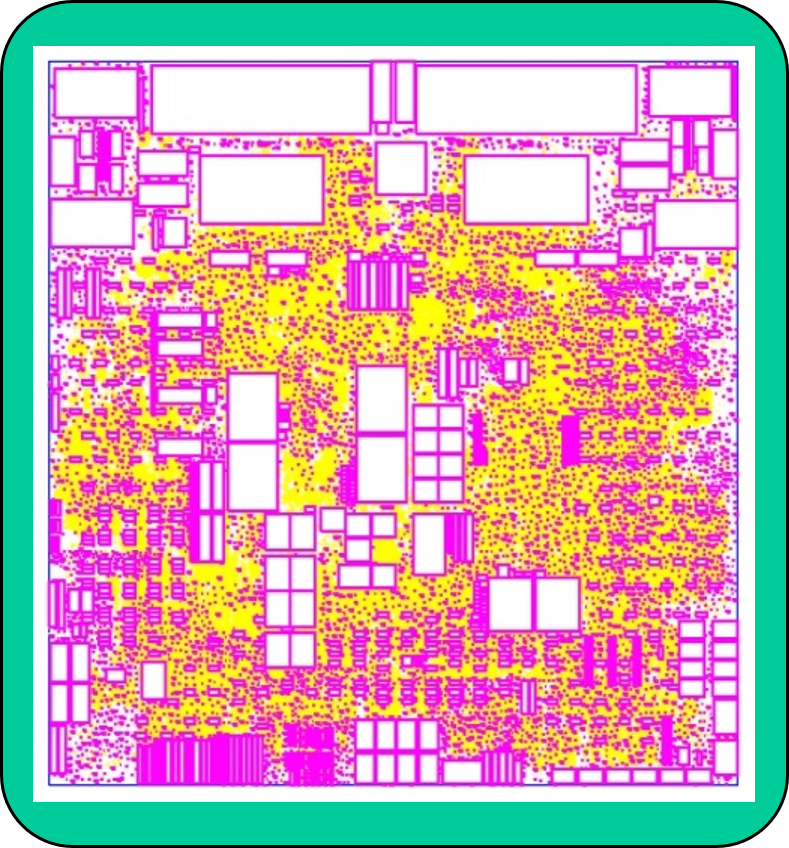
\includegraphics[width=0.6 \textwidth]{PP}
		\end{center}
		\column{0.7\textwidth}
		\begin{itemize}
			\item The quality of the attainable routing is highly determined by the placement.
			\item Circuit placement becomes very critical in  65nm and below technologies. 
		\end{itemize}
	\end{columns}
\end{frame}

\begin{frame}
	\frametitle{Placement}
	\textbf{Placement is the stage of the design flow, during which each standard cell is given an exact location}
	\pause
	\begin{itemize}
		\item Placement does not just place the standard cell available in the synthesized netlist, it also optimized the design.
		\pause
		\item \textbf{Inputs:}
		\pause
			\begin{enumerate}
				\item Netlist of gates and wires.
				\item Floorplan and Technology constraints
			\end{enumerate}
		\item \textbf{Outputs:}
		\pause
			\begin{enumerate}
			\item All cells located in the floorplan.
		\end{enumerate}
		\item \textbf{Goals:}
		\pause
		\begin{enumerate}
			\item Provide legal location of entire netlist
			\item Enable detailed route of all nets
			\item Meet timing, area, and power targets
		\end{enumerate}
	\end{itemize}
\end{frame}
%-----------------------------------------------------
\subsection[Flow]{Placement Flow}
\begin{frame}
	\frametitle{Global and Detailed Placement}
	\begin{itemize}
		\item In general, most tools partition the placement task
		into two stages:
	\end{itemize}
	\begin{center}
		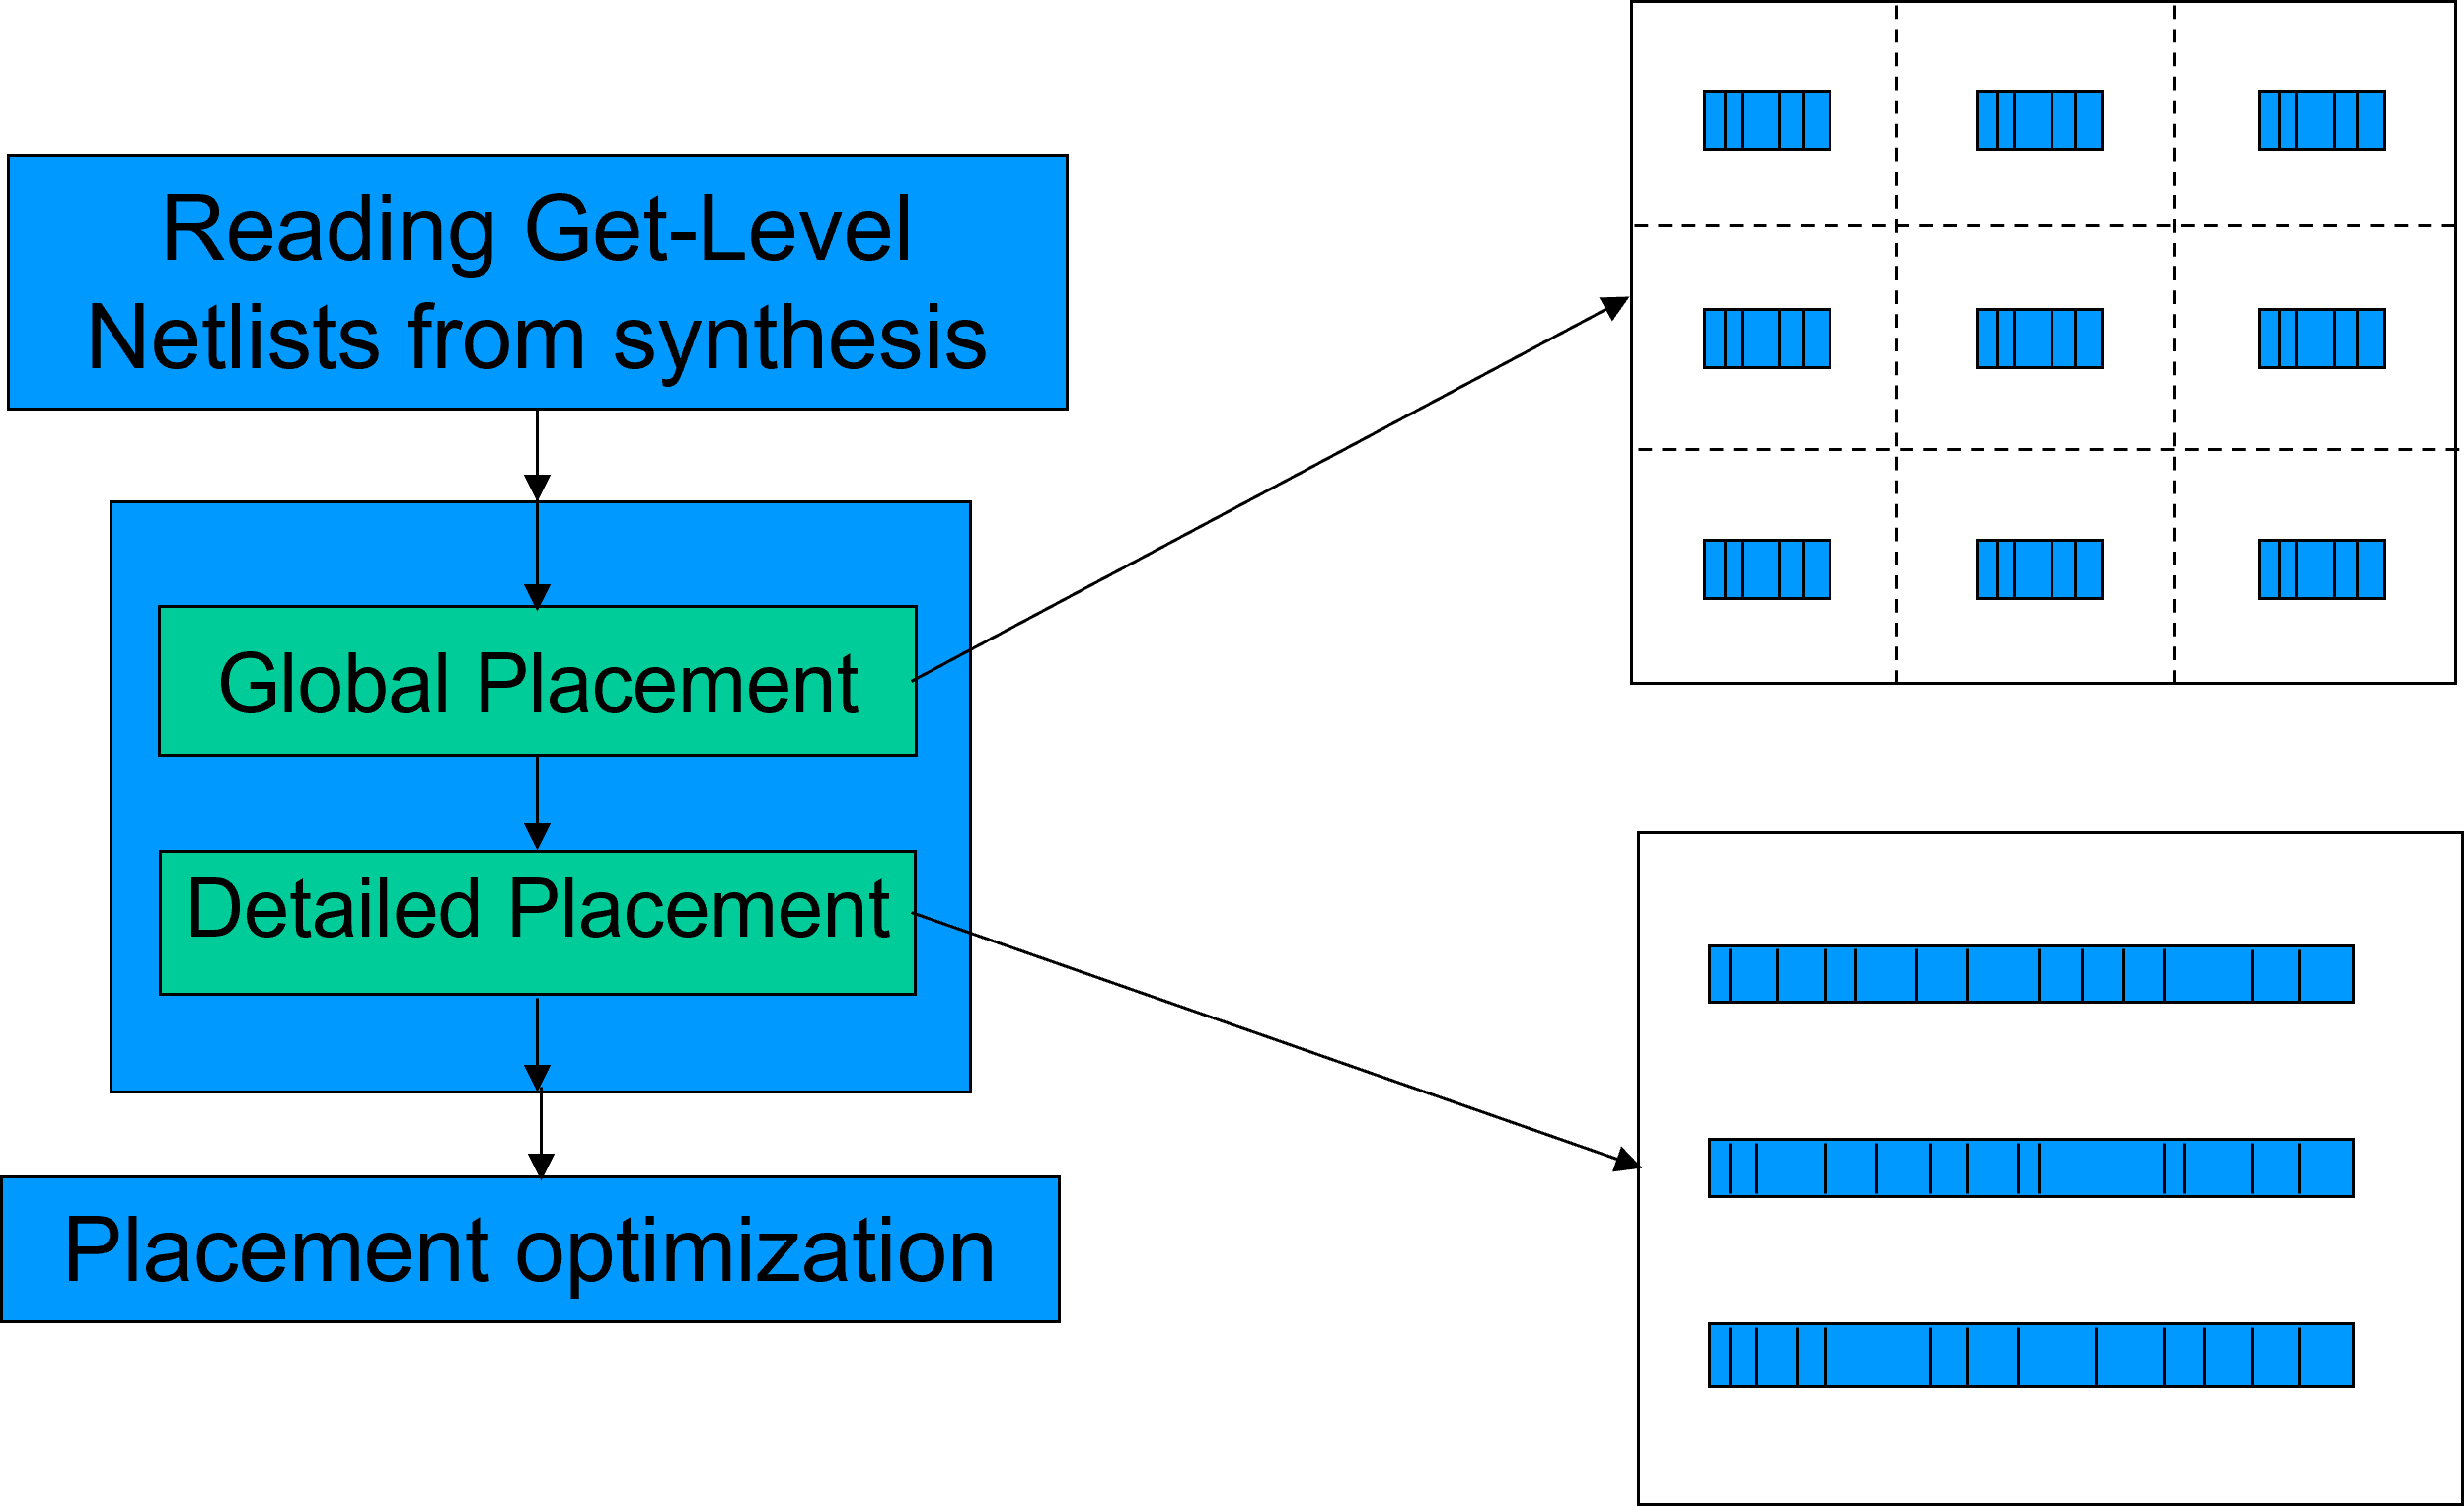
\includegraphics[width=0.8\textwidth]{PP2}
	\end{center}
\end{frame}

\begin{frame}
	\frametitle{Global Placement}
	\begin{itemize}
		\item Standard cells must be in groups in such a way that the number of connections between groups is minimum
		\pause
		\item This issue is solved through circuit partitioning \pause
		\item As a basic criterion, the minimum is taken among group connections
	\end{itemize}
		\begin{center}
			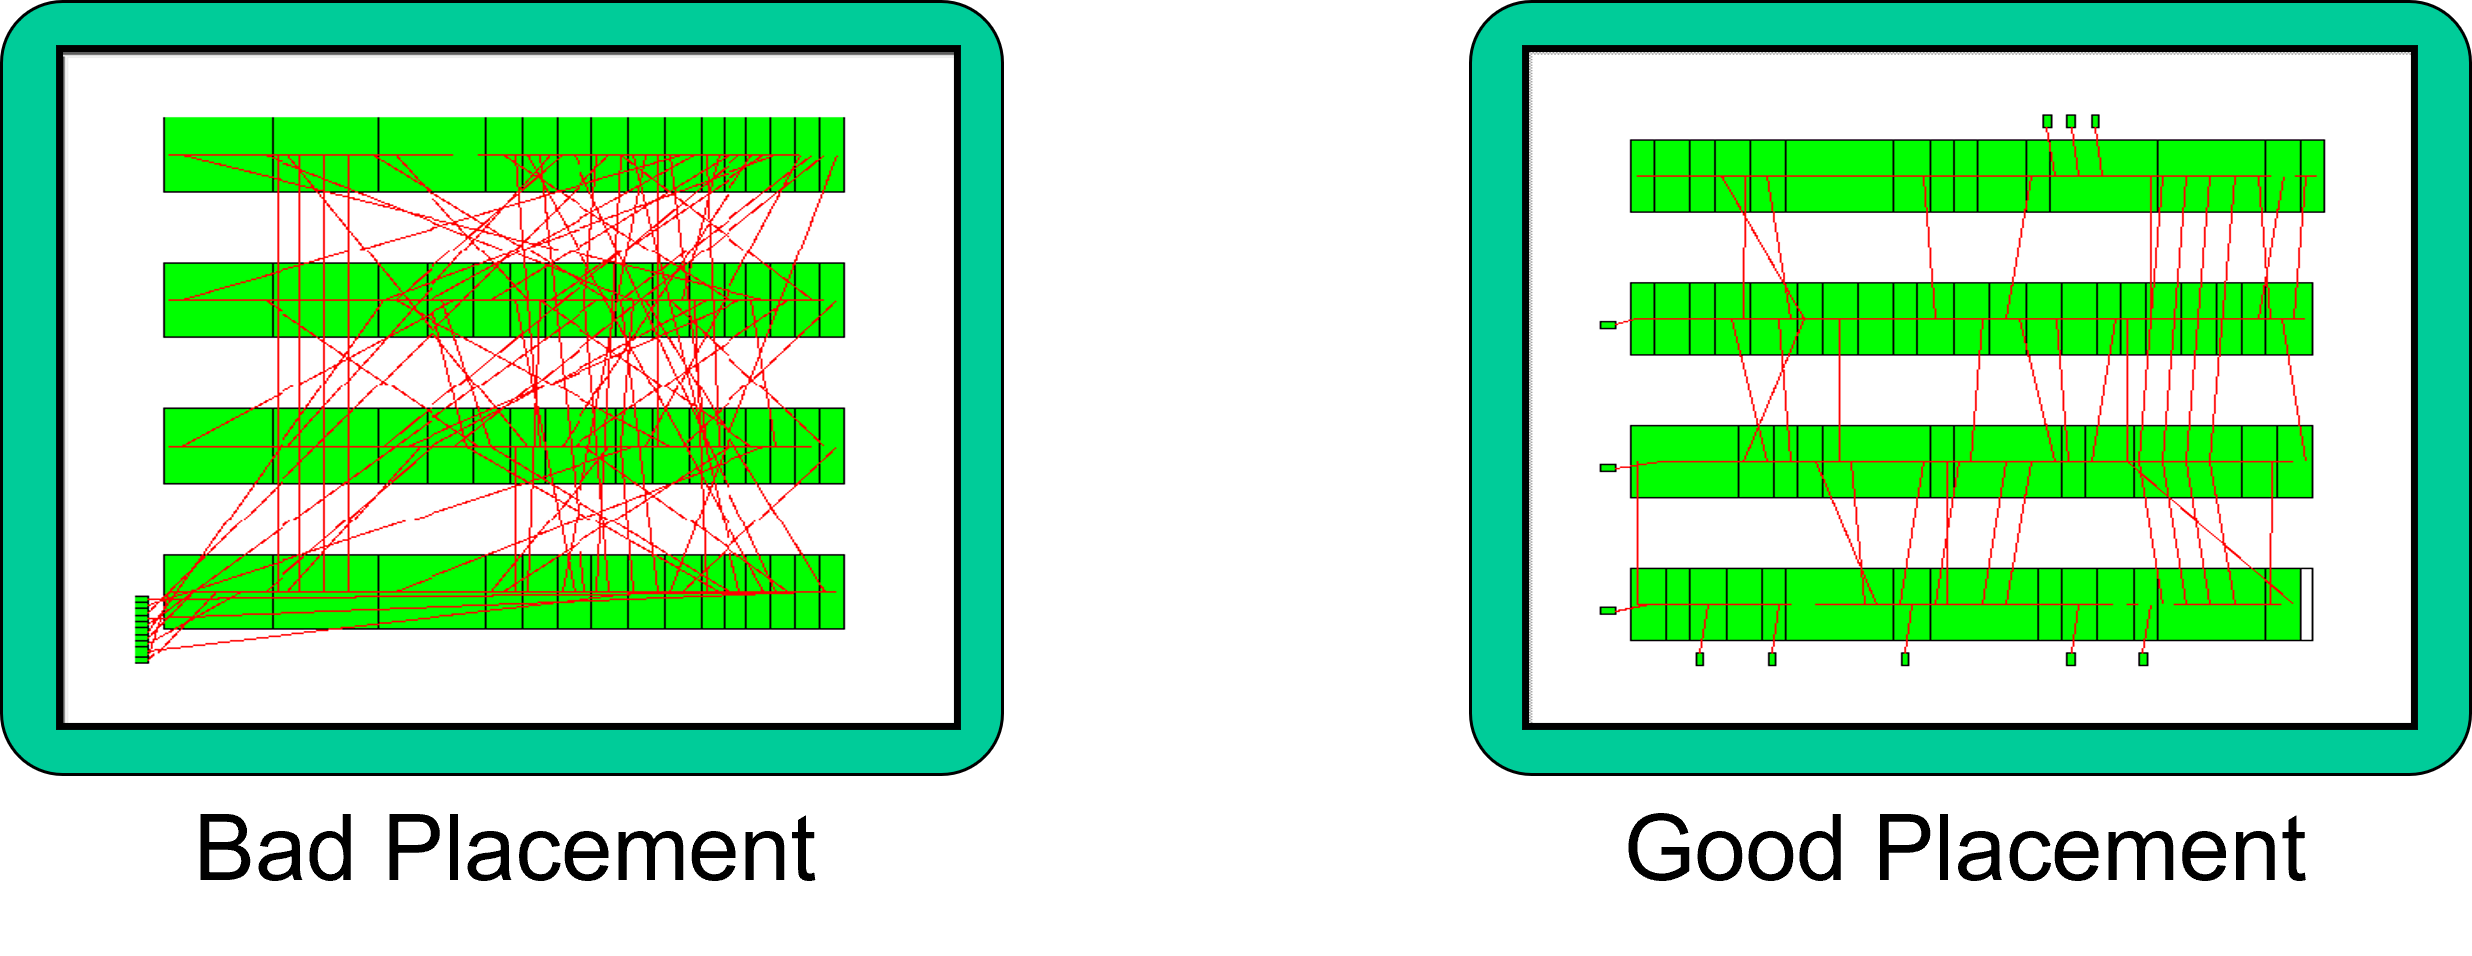
\includegraphics[width=0.7\textwidth]{good_bad}
		\end{center}
\end{frame}
\begin{frame}
	\frametitle{Detailed Placement}
	\begin{columns}	
		\column{0.7\textwidth}
		\begin{center}
			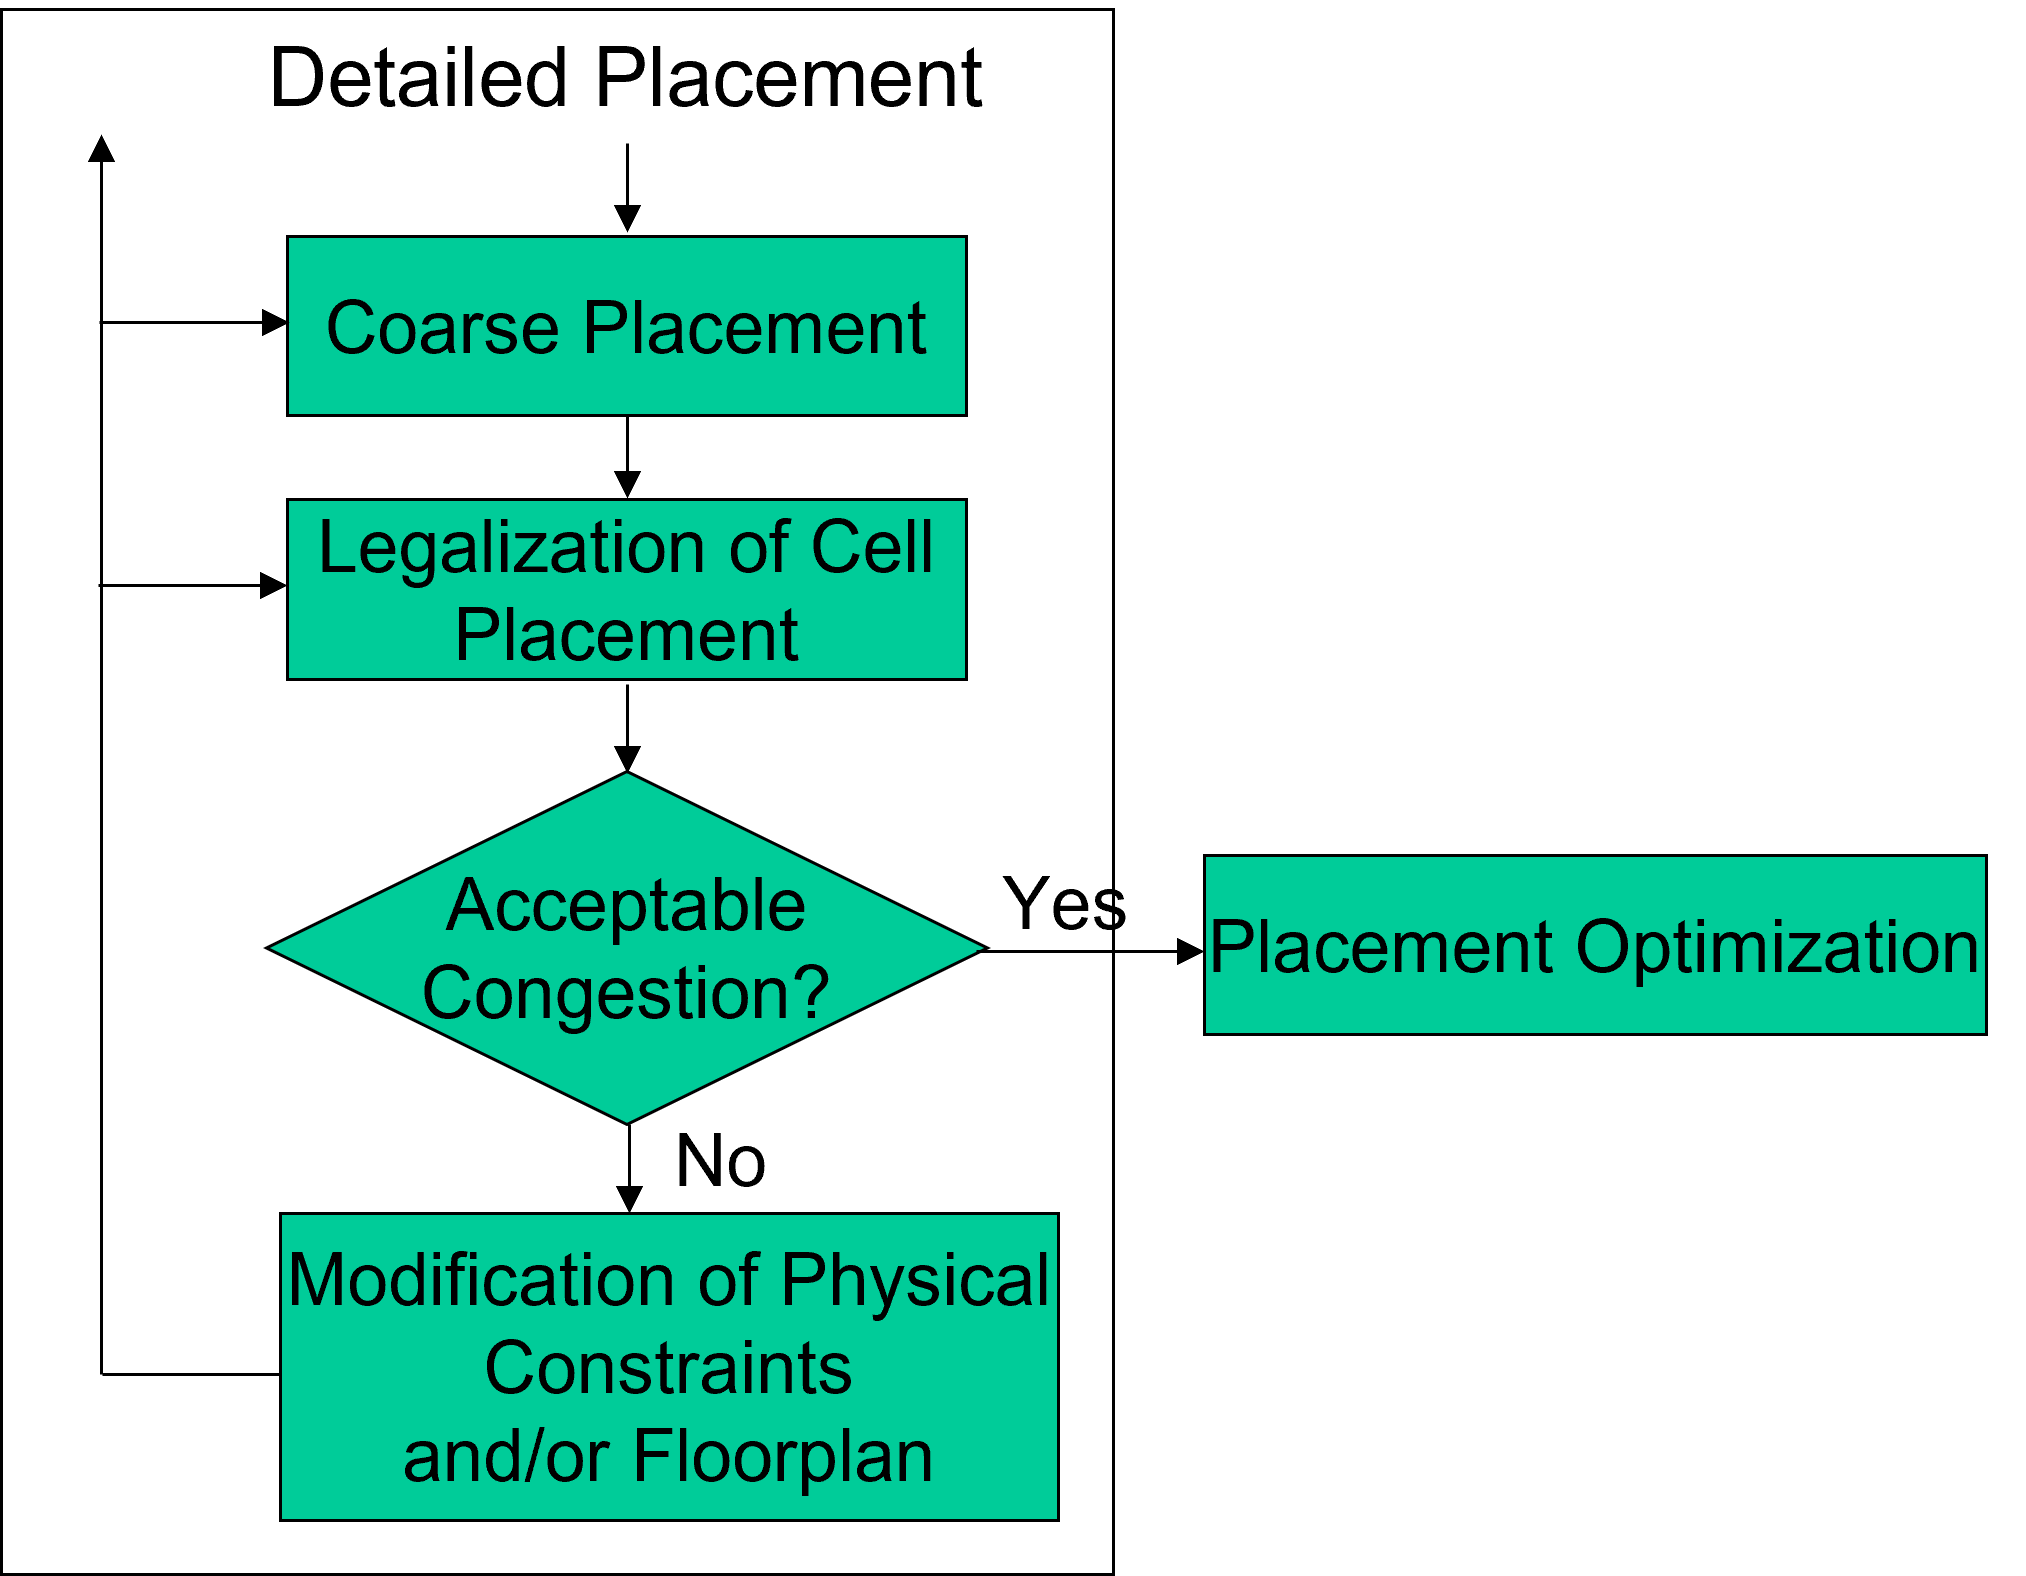
\includegraphics[width=0.8 \textwidth]{DP}
		\end{center}
		\column{0.5\textwidth}
		\begin{itemize}
			\item As a rule, detailed placement is solved in two stages: 
			\begin{enumerate}
				\item Coarse placement
				\item Legalization of cell placement
			\end{enumerate}
		\end{itemize}
	\end{columns}
\end{frame}

\begin{frame}
	\frametitle{Coarse placement}
	\begin{center}
		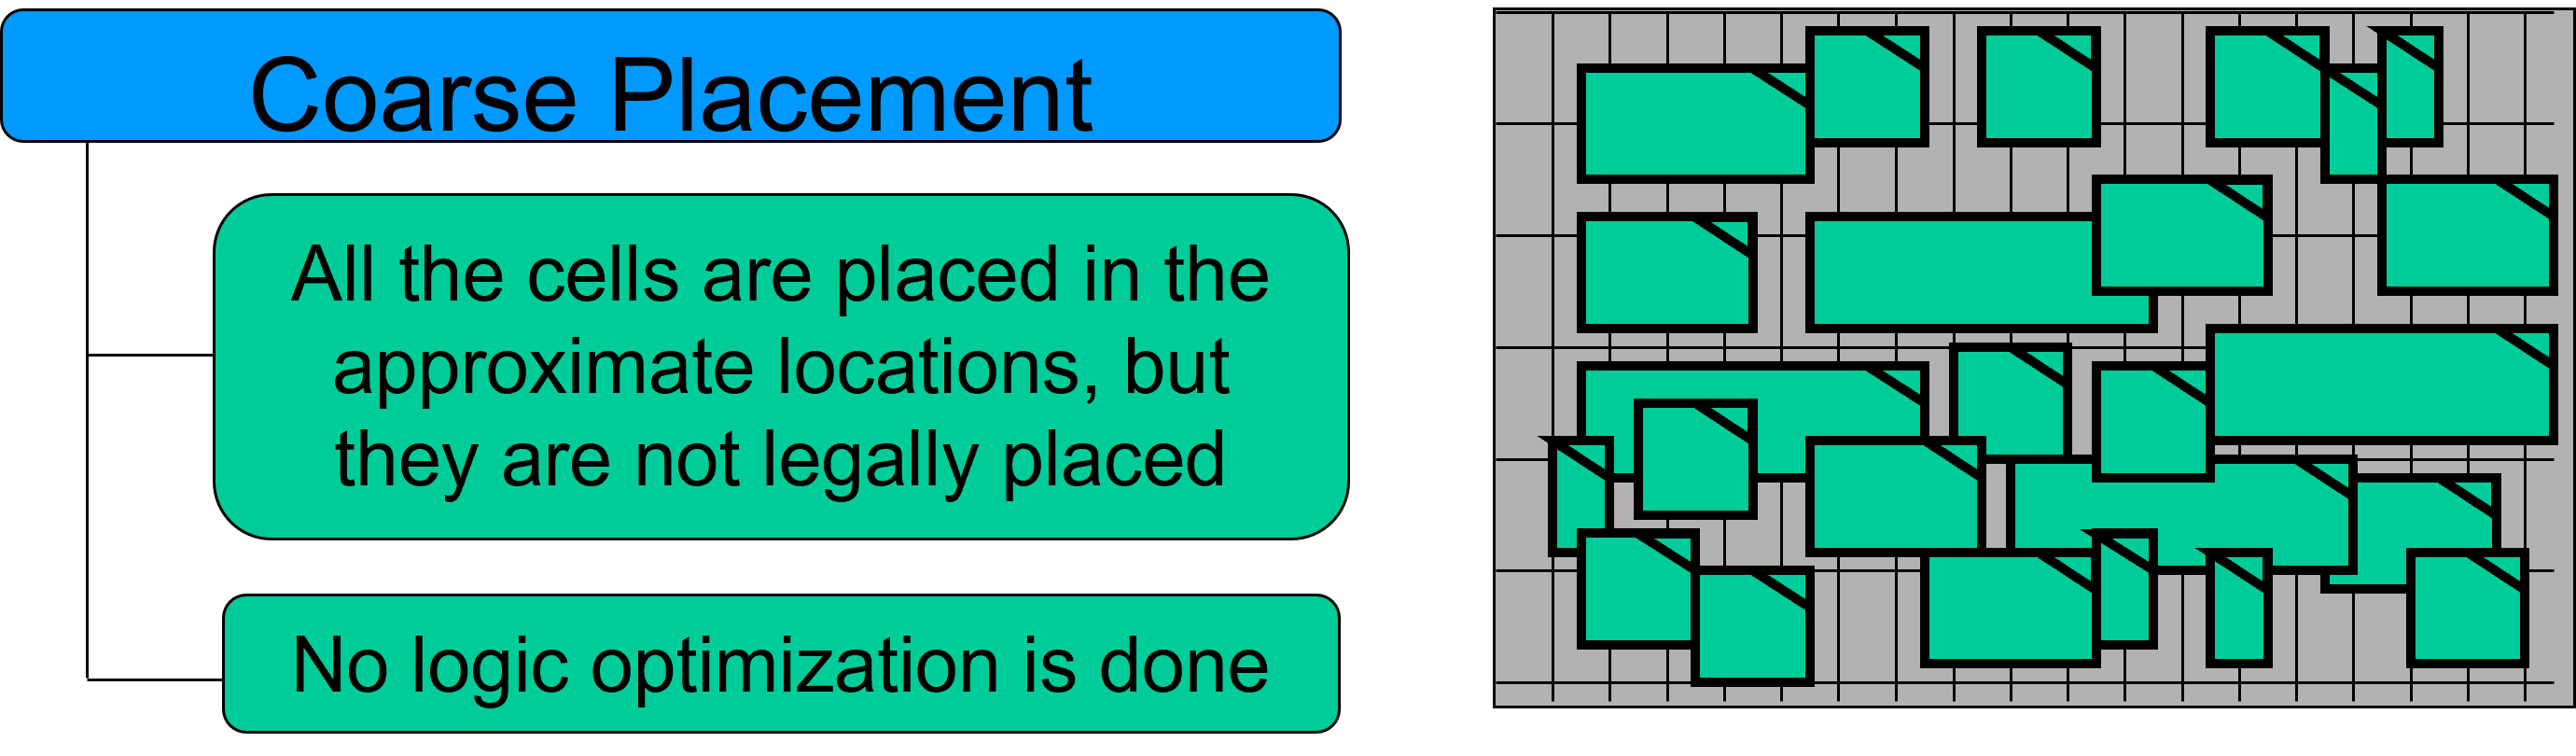
\includegraphics[width=0.7\textwidth]{CP}
	\end{center}
\begin{itemize}
	\item In a coarse placement all the cells are placed in the approximate locations but they are not legally placed. 
	\item Cells overlap and are not on-grid. 
	\item Large cells (e.g. RAMs) form large placement blockages for other smaller leaf cells. 
	\item Power routing forms routing layer blockages that will also be checked and avoided if specified.
	
\end{itemize}
\end{frame}

\begin{frame}
	\frametitle{Legalize Cell Placement}
	\begin{center}
		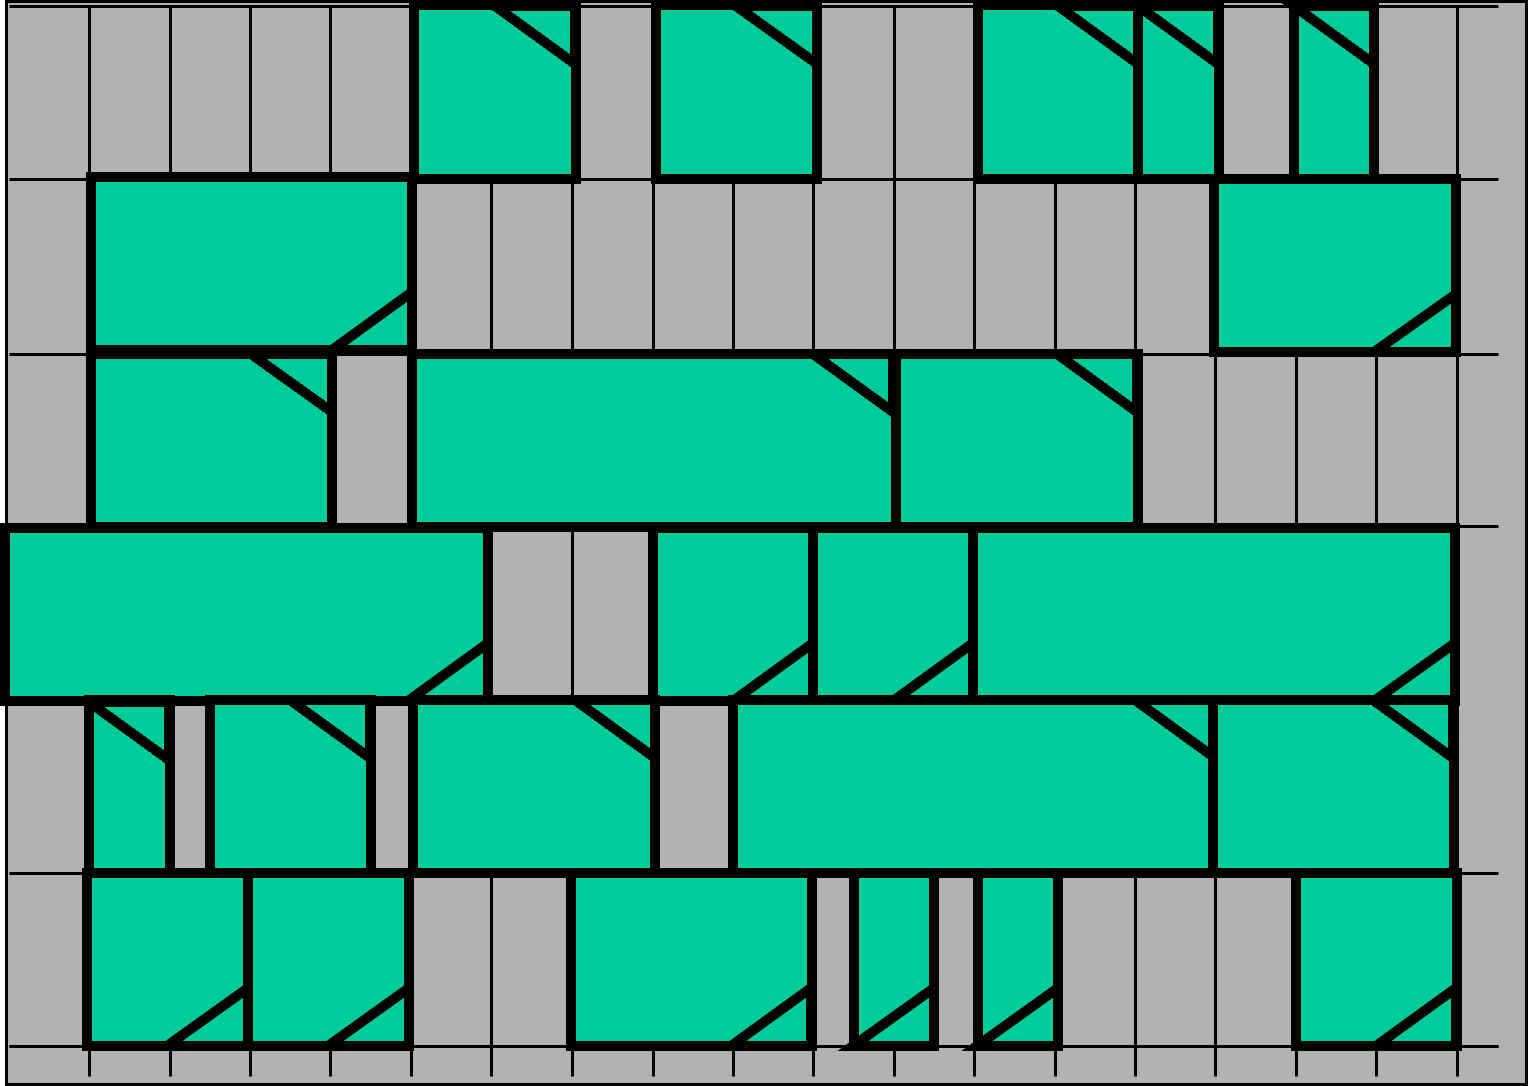
\includegraphics[width=0.6\textwidth]{lp}
	\end{center}
\begin{itemize}
	\item Provide a legal placement for each instance with no overlap
	\item Try and minimize wirelength (or other cost metrics)
	\item Try to finish with uncongested design
\end{itemize}
\end{frame}

%-------------------------------------------------
\section[TDP]{Timing Driven Placement}
	\subsection[Timing]{Timing-Driven Placement}
	\begin{frame}
		\frametitle{Timing-Driven Placement (1)}
		\begin{columns}	
			\column{0.6\textwidth}
		\begin{itemize}
			\item All steps including placement are timing-driven
			
			\item Timing-driven placement tries to place critical path cells close together to reduce net  RCs and to meet setup timing
			\item RCs are based on Virtual Route (VR)
			
		\end{itemize}
	\column{0.7\textwidth}
	\begin{center}
		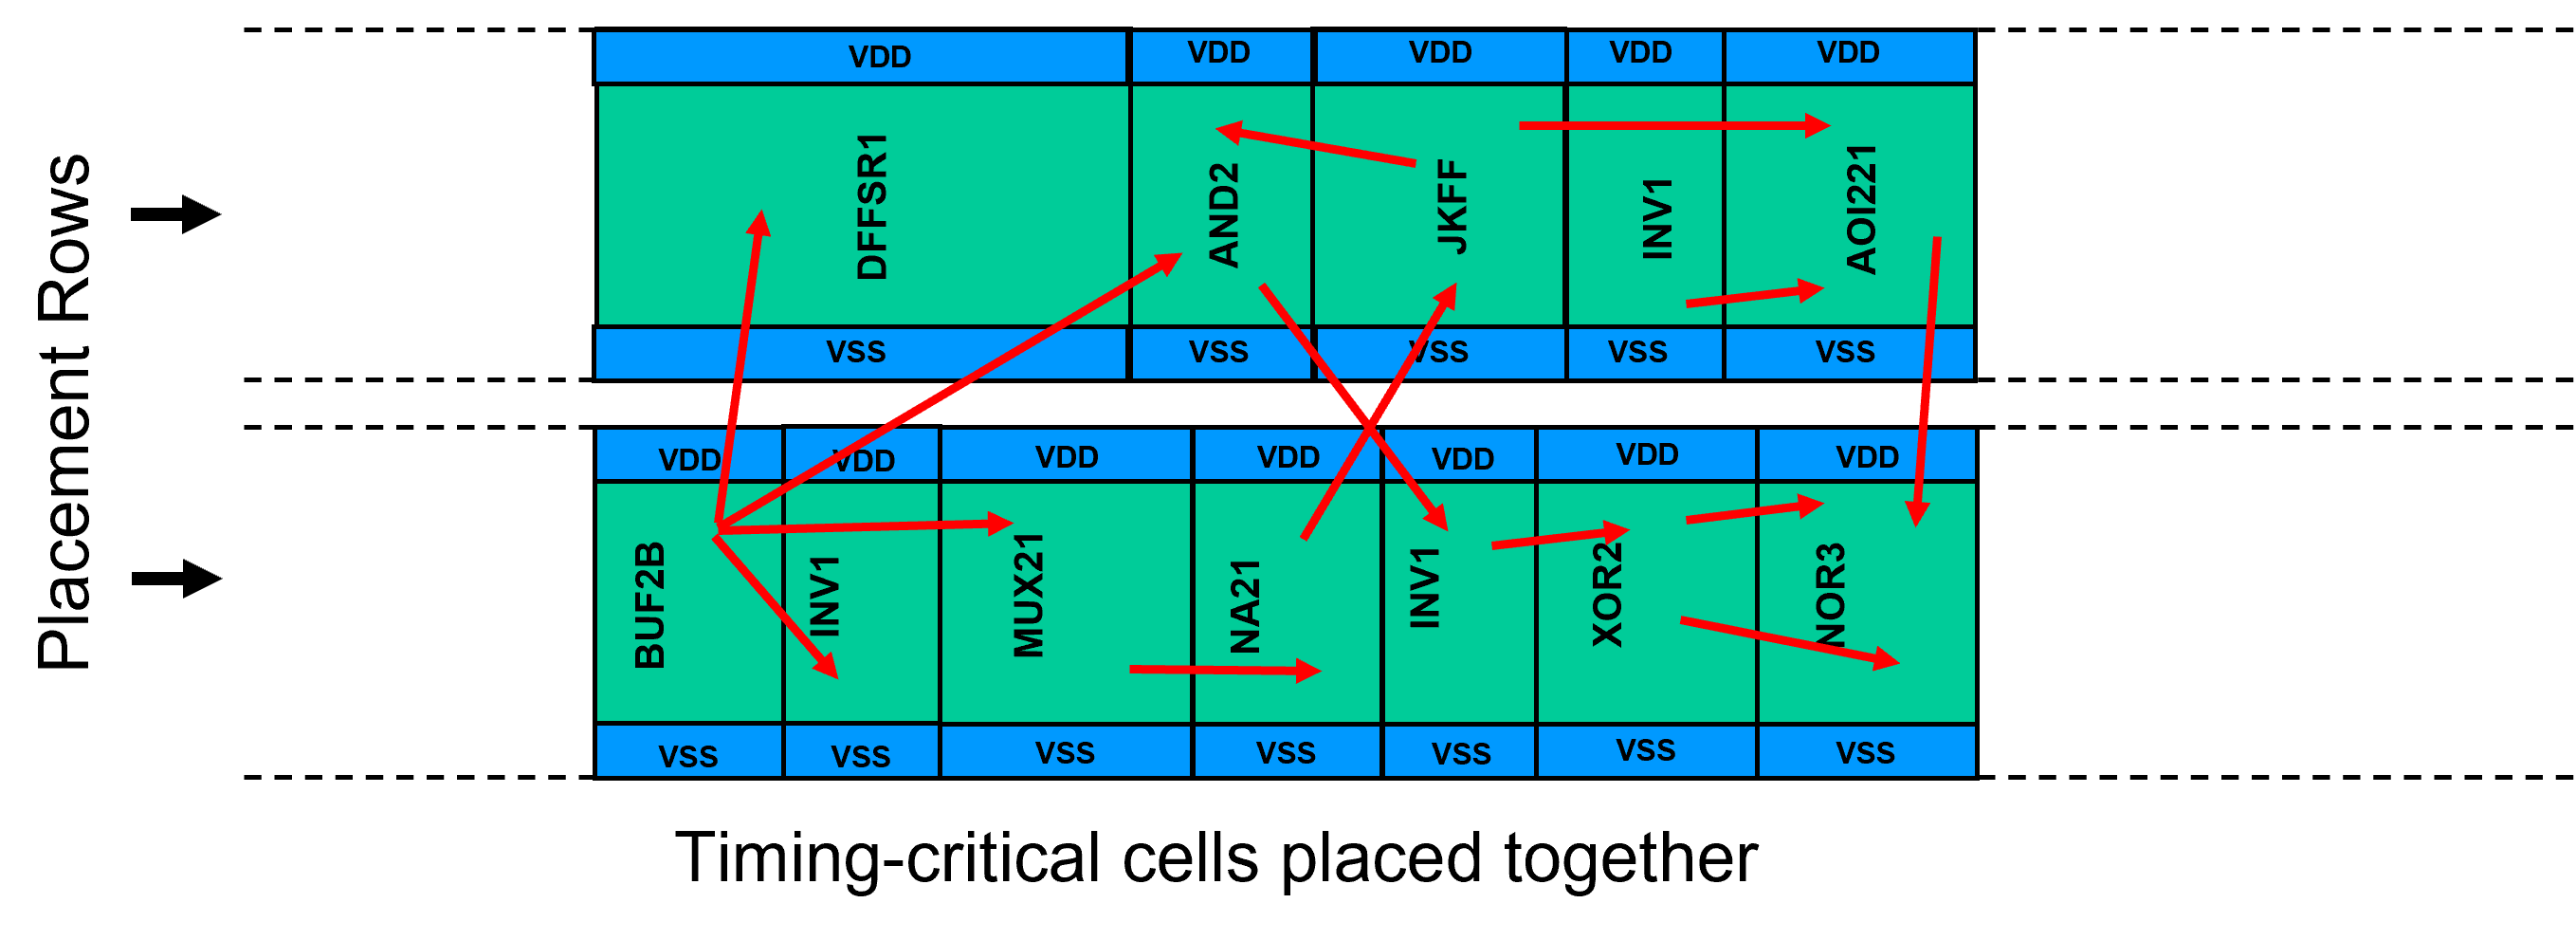
\includegraphics[width=0.7\textwidth]{TDP}
	\end{center}
\end{columns}
	\end{frame}
\begin{frame}
	\frametitle{Timing-Driven Placement (2)}
	\begin{columns}	
		\column{0.5\textwidth}
		\begin{itemize}
			\item Timing-driven placement based on Virtual Route
			
			\begin{itemize}
			\item Tries to place cells along timing-critical paths close together to reduce net RCs and meet setup timing
			
			\item Net RCs are based on Virtual Routing (VR) estimates
			
			\end{itemize}
			
		\end{itemize}
		\column{0.5\textwidth}
		\begin{center}
			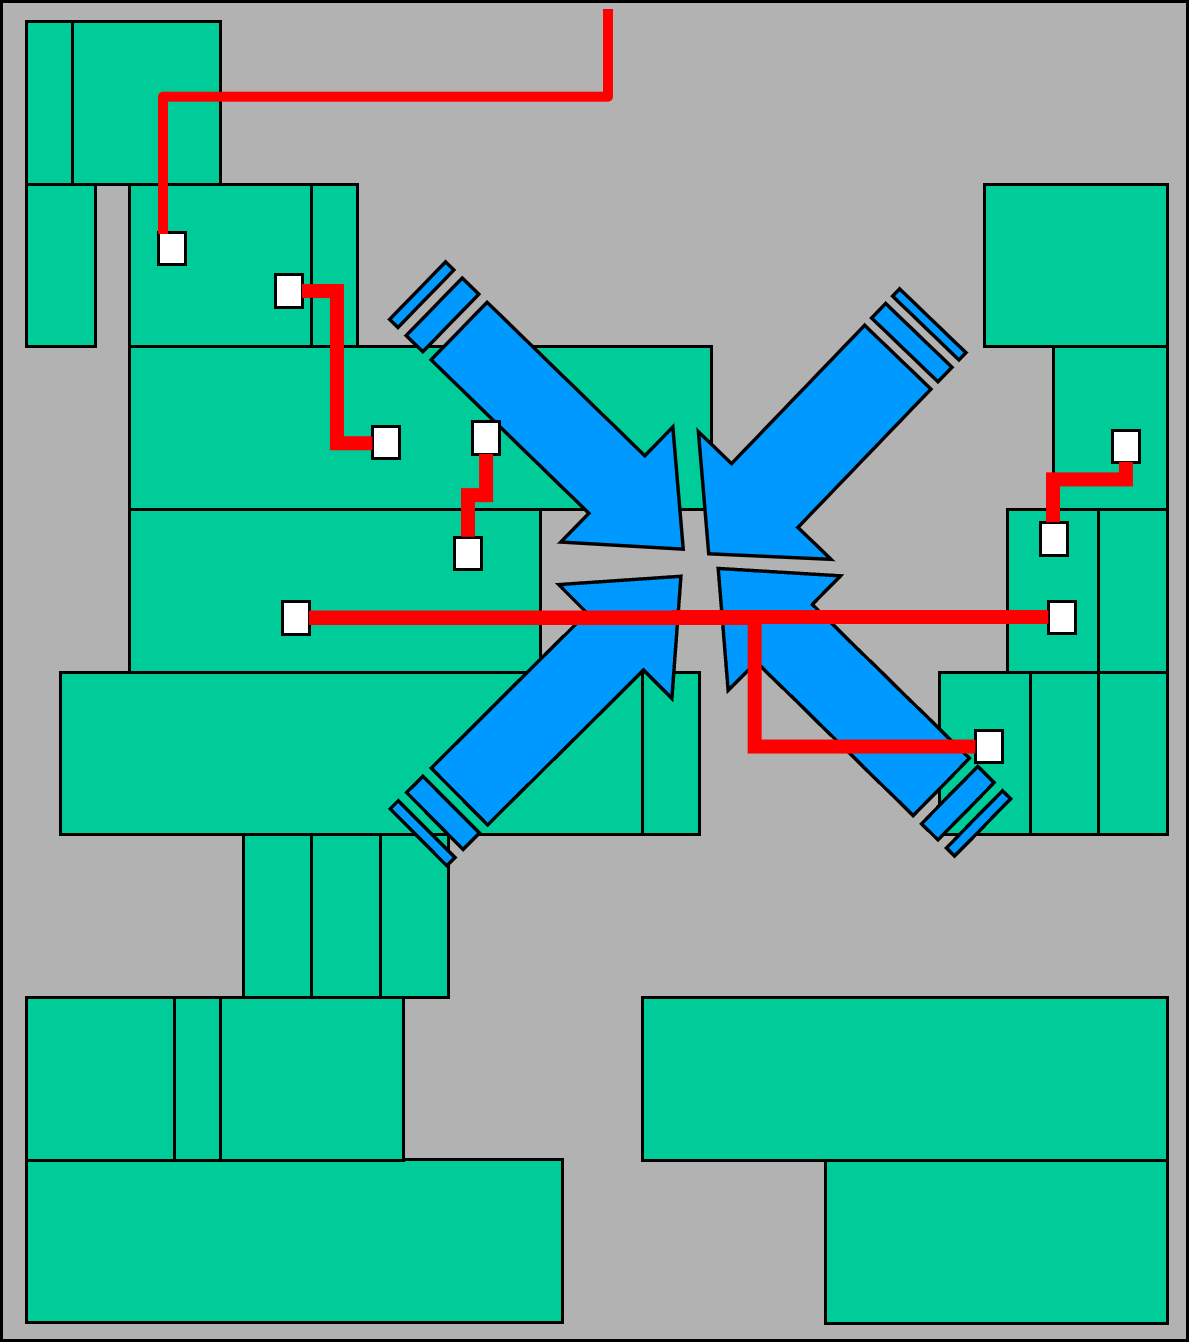
\includegraphics[width=0.8\textwidth]{TDP2}
		\end{center}
	\end{columns}
\end{frame}

\begin{frame}
	\frametitle{Timing-Driven Placement (3)}
	\begin{itemize}
		\item Standard cells are placed in “placement rows”
		\item Cells in a timing-critical path are placed close together to reduce routing-related delays$\,\to\,$Timing-Driven Placement
		
	\end{itemize}
	\begin{center}
		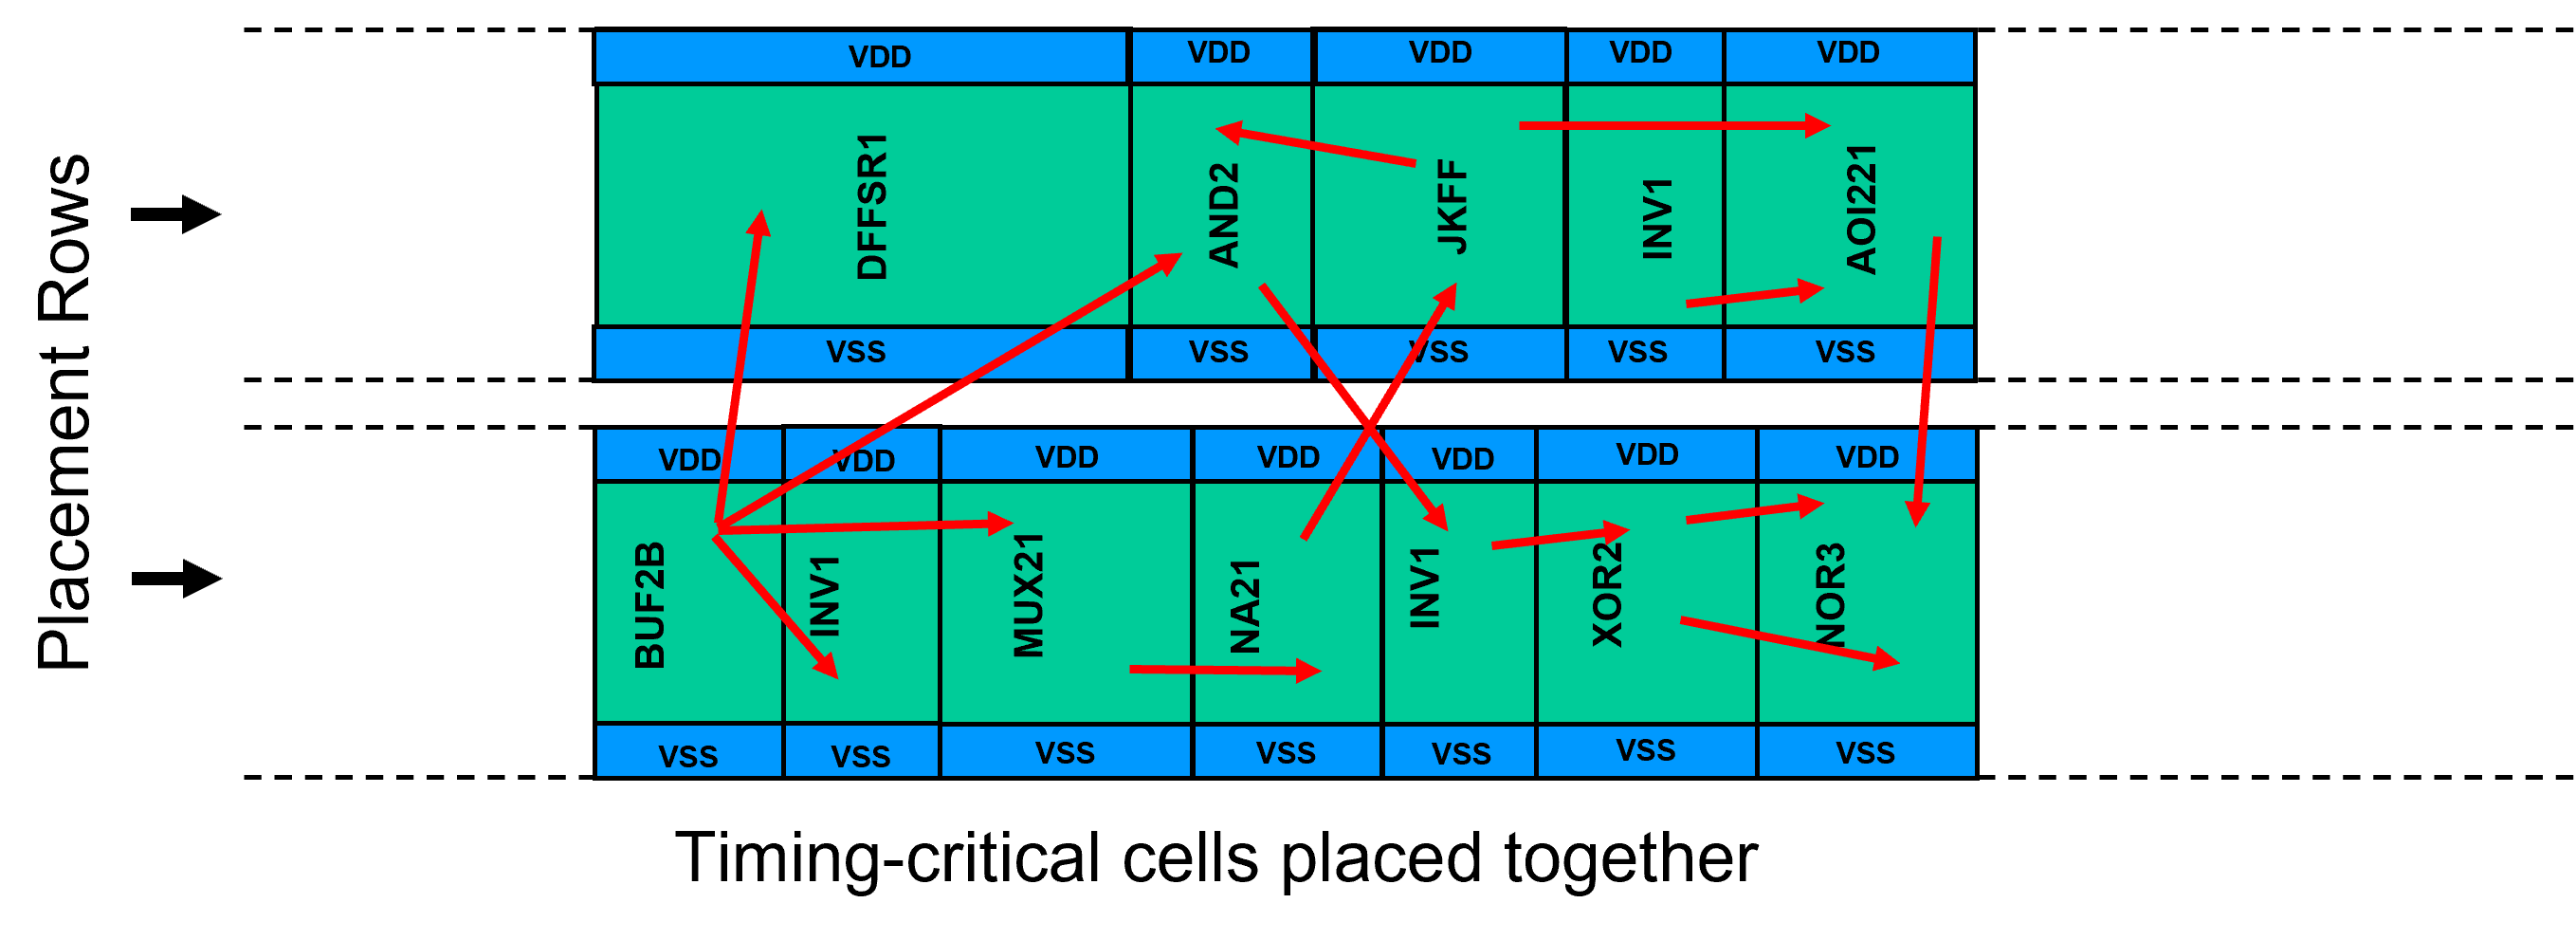
\includegraphics[width=0.8\textwidth]{TDP3}
	\end{center}
\end{frame}

\begin{frame}
	\frametitle{TDP: Estimating Rnet and Cnet Before Placement}
	\begin{center}
		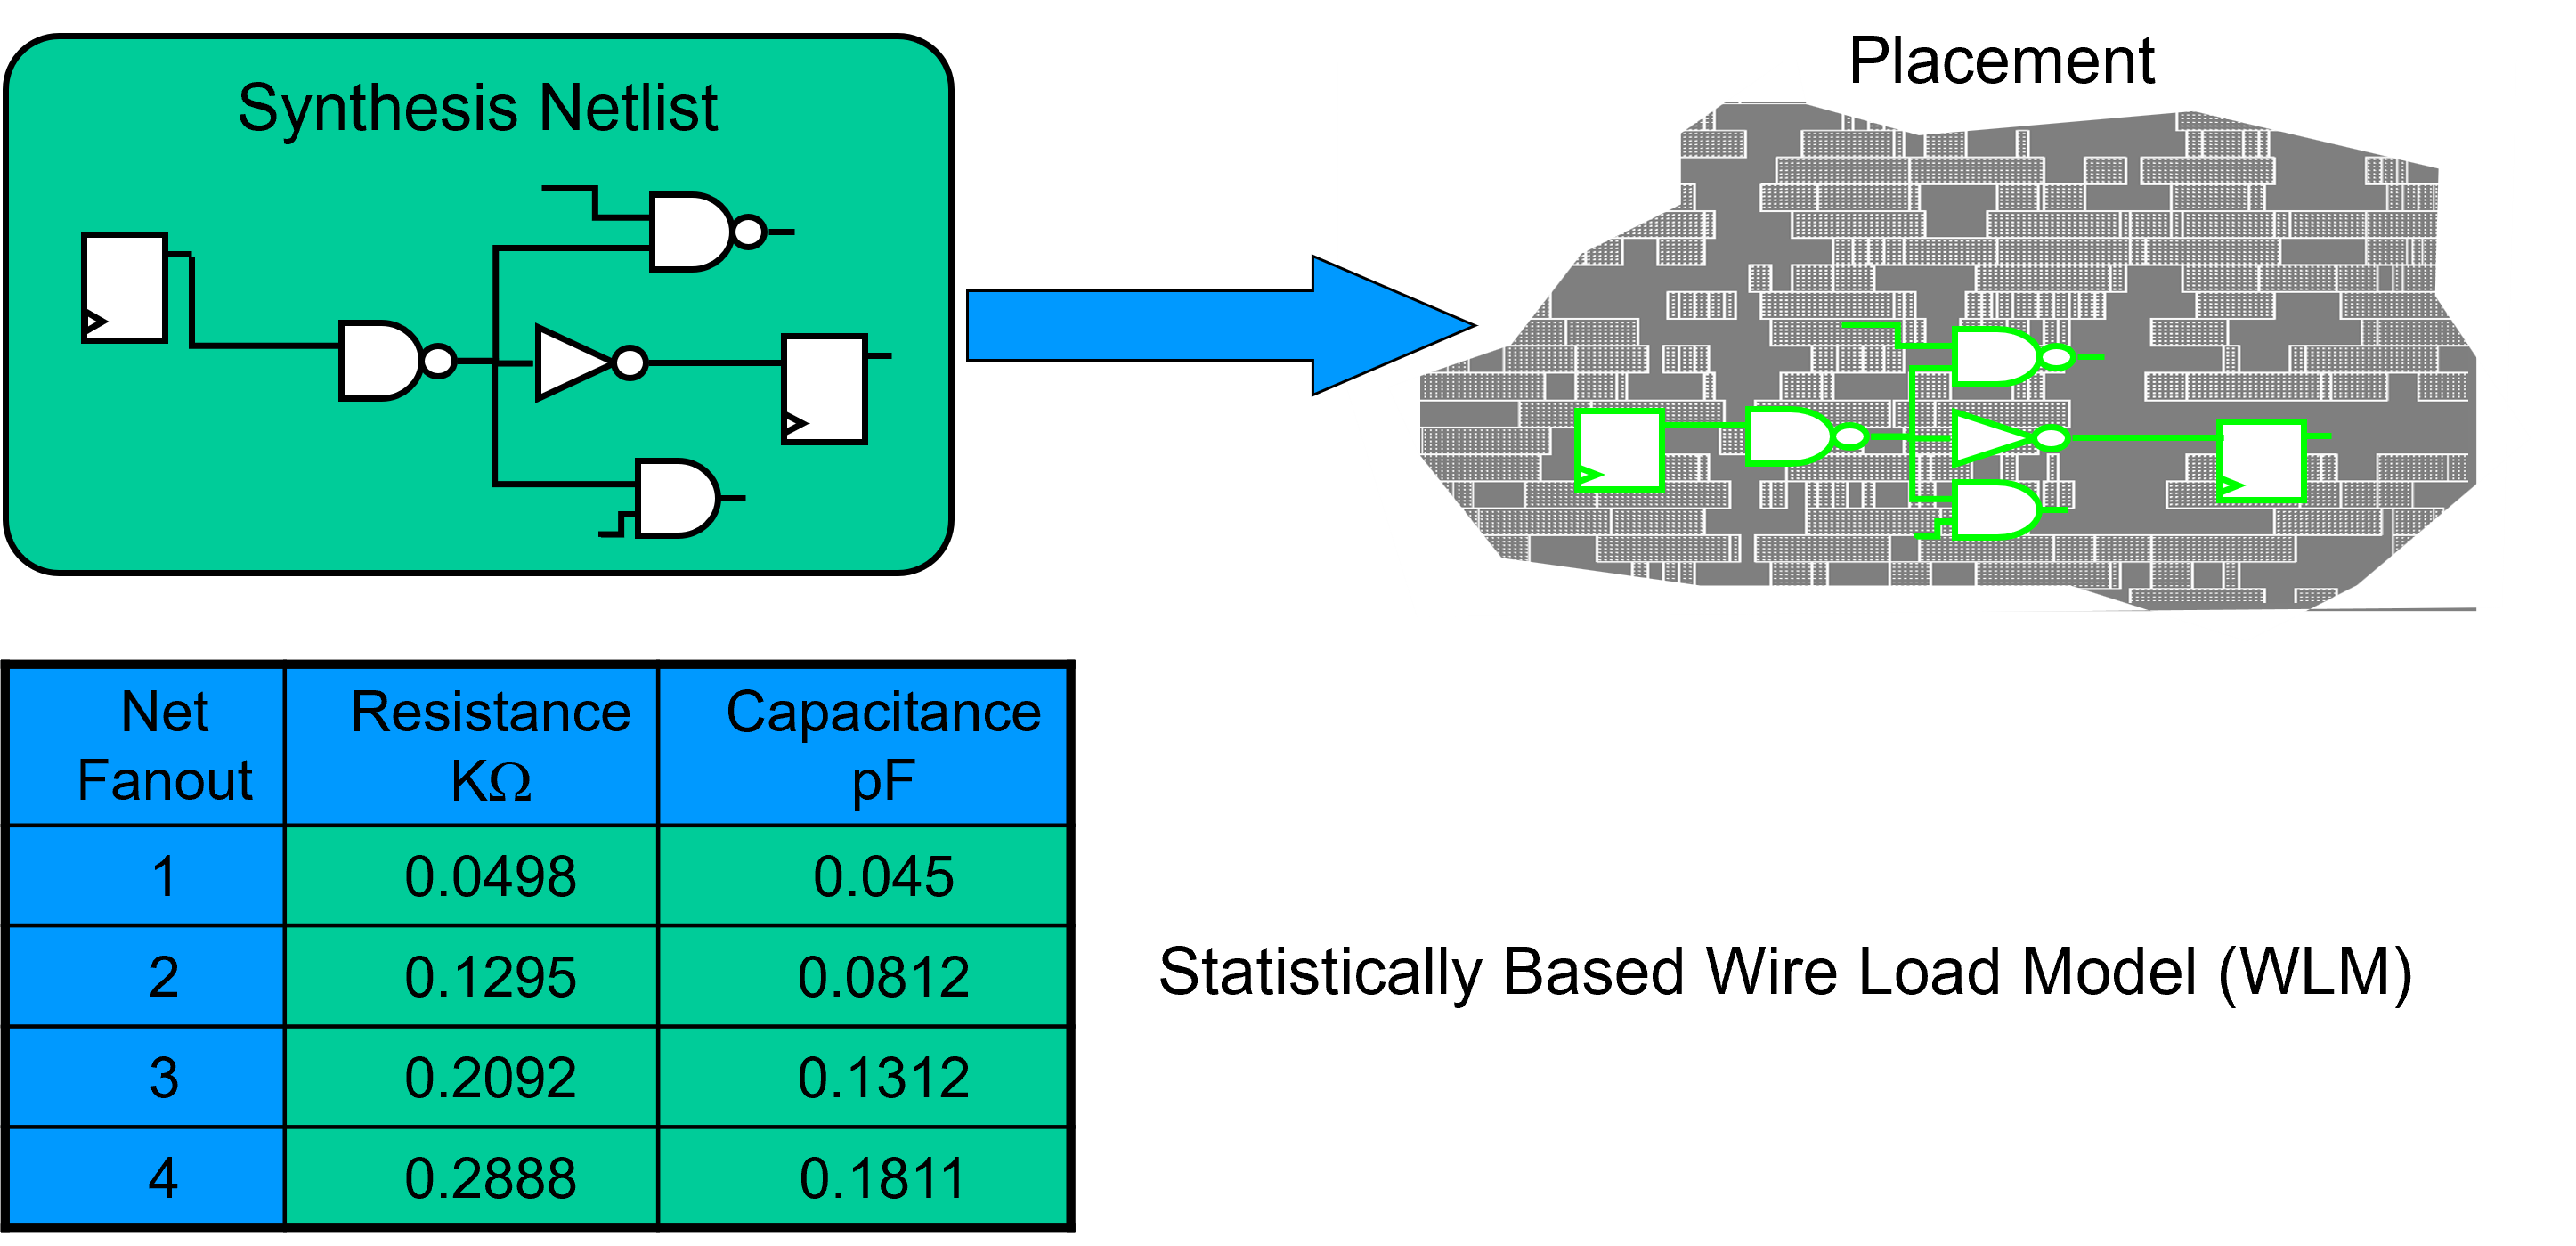
\includegraphics[width=\textwidth]{TDP4}
	\end{center}
\end{frame}
%-----------------------------------------------------

-
\section[Congestion]{Congestion Driven Placement}
\subsection[Congestion]{Congestion Driven Placement}
\begin{frame}
	\frametitle{Congestion}
	\begin{itemize}
		\item Congestion occurs when the number of required
		routing tracks exceeds the number of available tracks.
		\begin{itemize}
			\item Congestion can be estimated from
			the results of a quick global route.
			\item Global bins with routing overflow
			can be identified
		\end{itemize}
	\end{itemize}
\begin{center}
	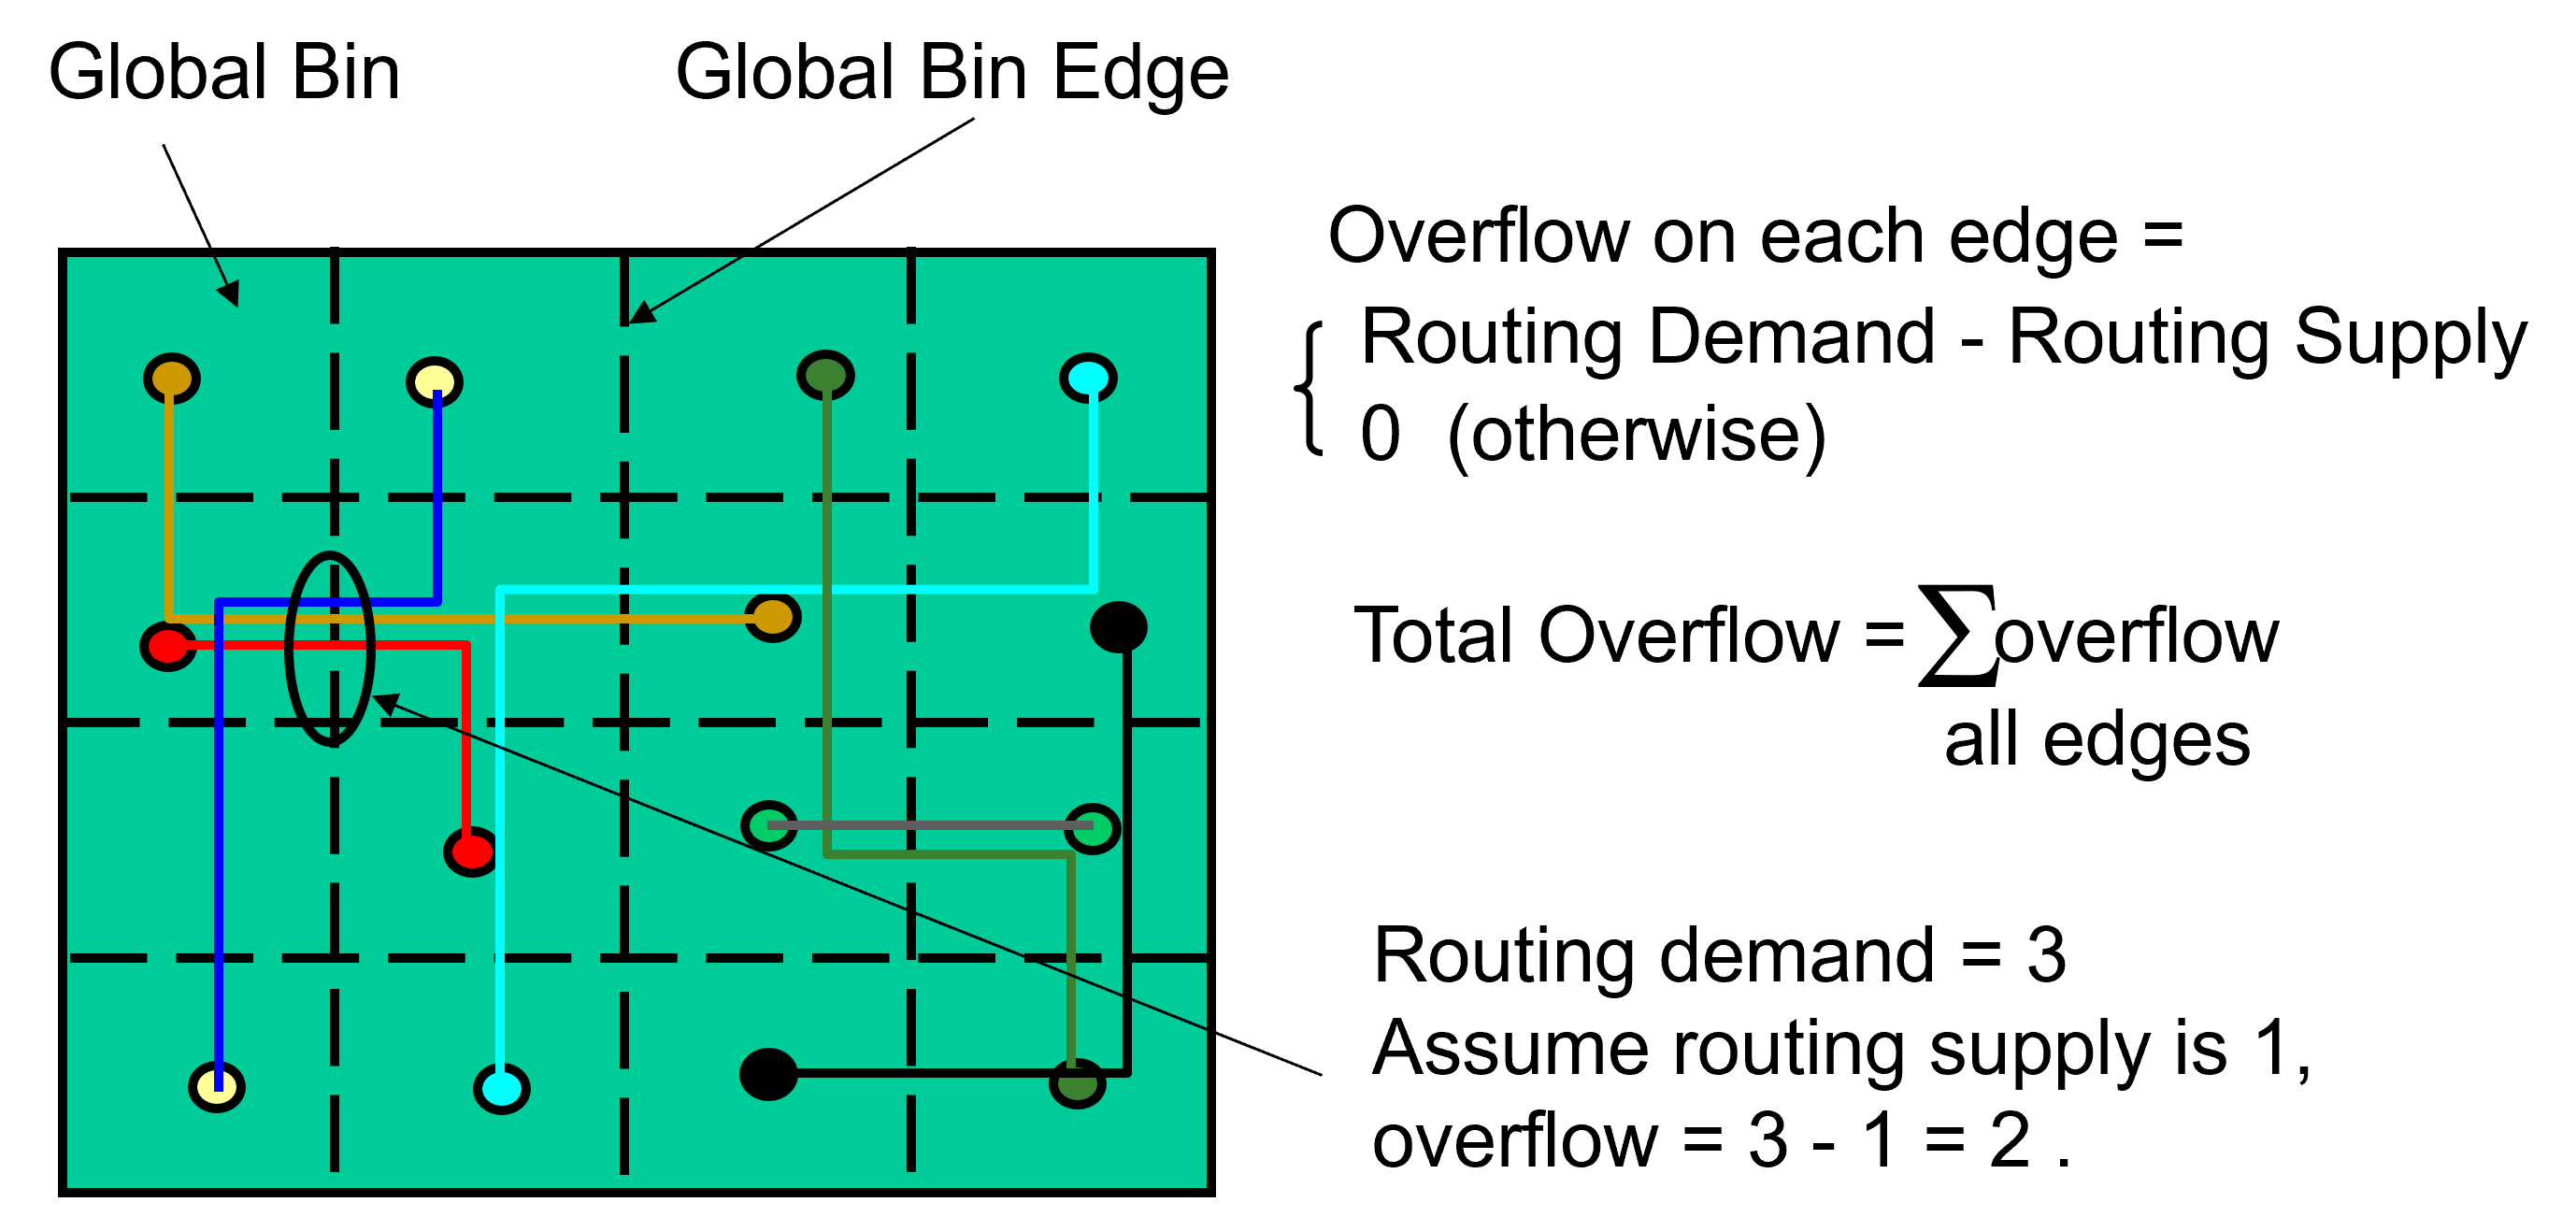
\includegraphics[width=0.8\textwidth]{CDP}
\end{center}
\end{frame}

\begin{frame}
	\frametitle{Congestion Driven Placement: Routing resource}
		\begin{center}
			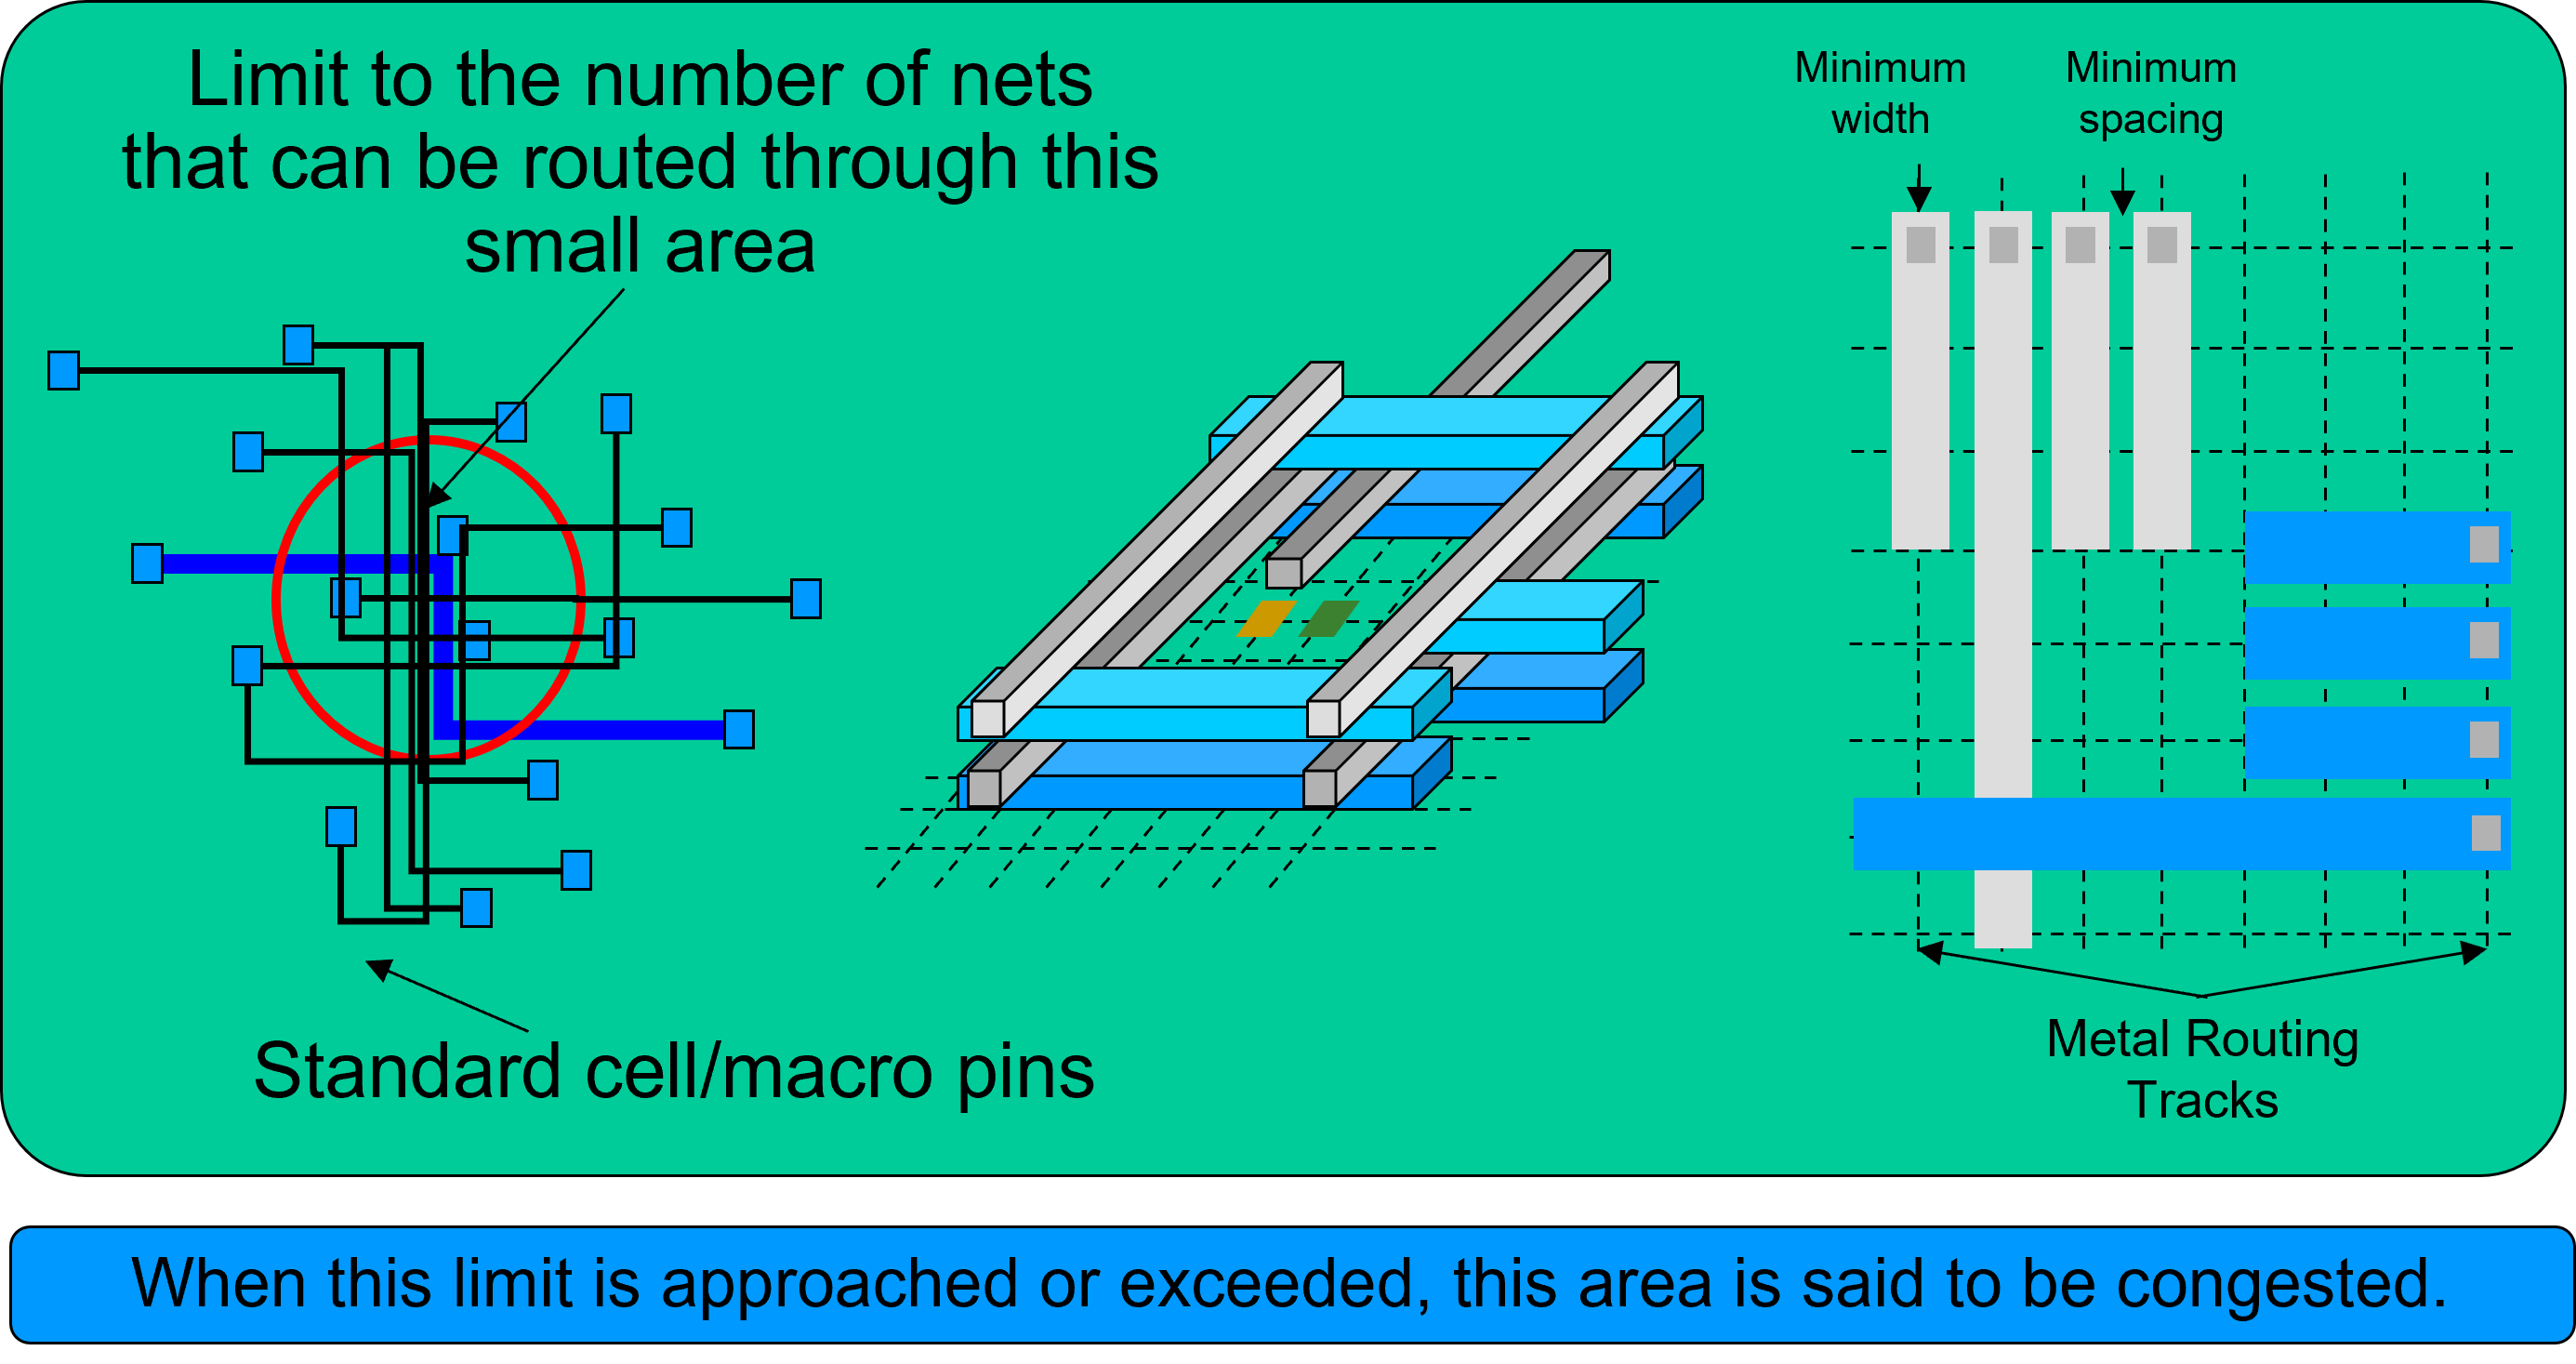
\includegraphics[width=\textwidth]{RS}
		\end{center}
\end{frame}
\subsection[Issues]{Placement Issues with Congestion}
\begin{frame}
	\frametitle{Placement Issues with Congestion}
	\begin{columns}
		\column{0.6 \textwidth}
			\begin{itemize}
				\item If congestion is not too severe, the actual route can be detoured around the congested area
				\item The detoured nets will have worse RC delay compared to the VR estimates
			\end{itemize}
		\column{0.5 \textwidth}
			\begin{center}
				\includegraphics[width=0.8 \textwidth]{congestion}
			\end{center}
	\end{columns}
	\begin{alertblock}{congested}
	In highly congested areas, delay estimates during placement will be optimistic.
\end{alertblock}
\end{frame}

\begin{frame}
	\frametitle{Non Routable on Severely Congested Design}
		\begin{columns}
		\column{0.6 \textwidth}
		\begin{itemize}
			\item It is important to minimize or eliminate congestion before continuing
			
			\item Severe congestion can cause a design to be un-routable
			
		\end{itemize}
		\column{0.5 \textwidth}
		\begin{center}
			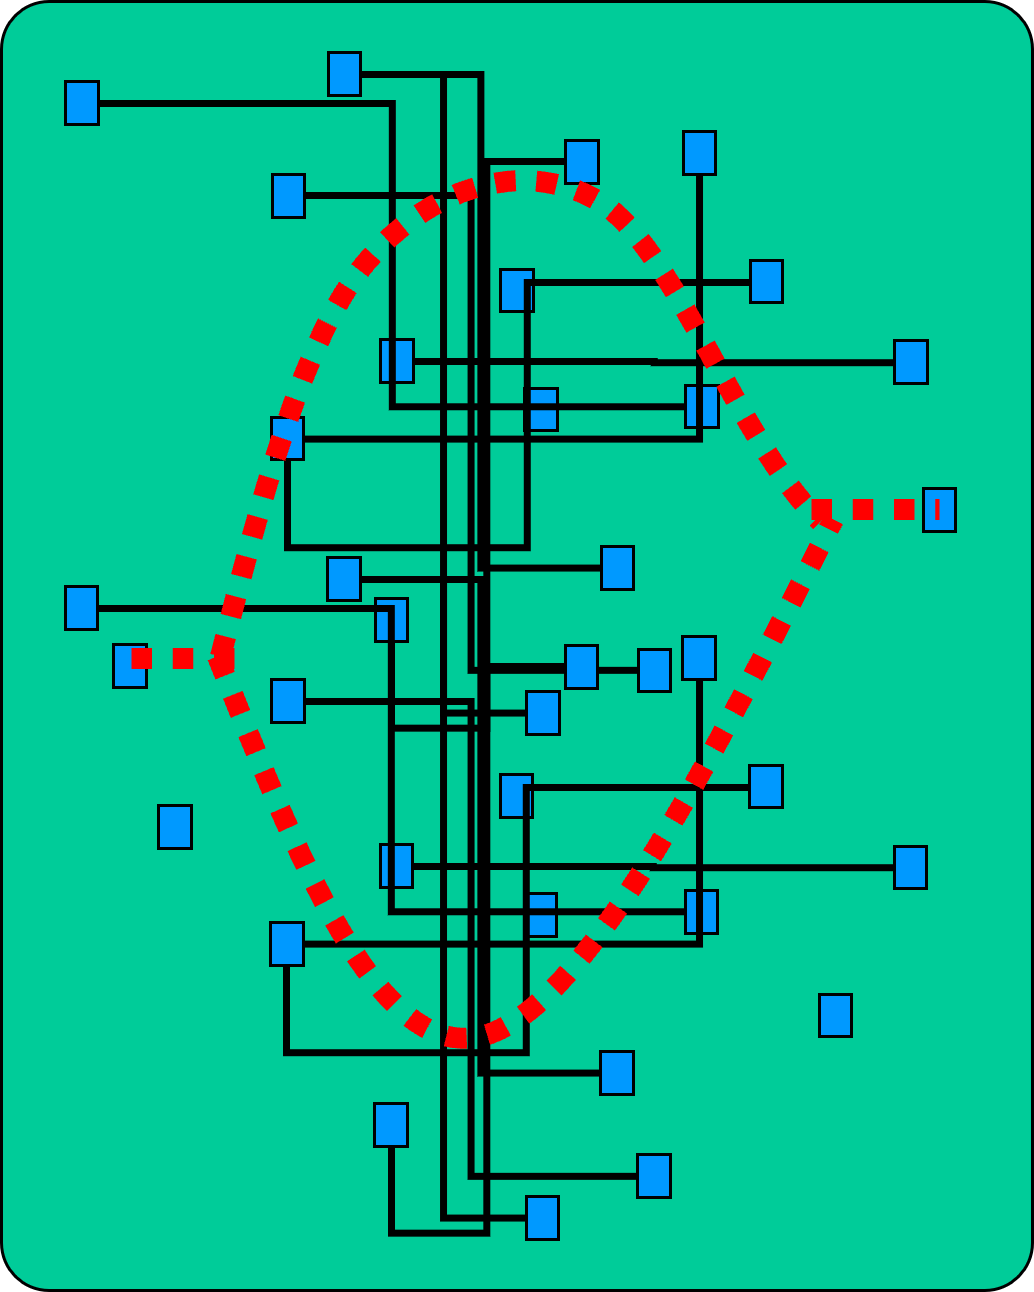
\includegraphics[width=0.8 \textwidth]{un-routable}
		\end{center}
	\end{columns}
\end{frame}

\begin{frame}
	\frametitle{Congestion Calculation}
	\begin{center}
		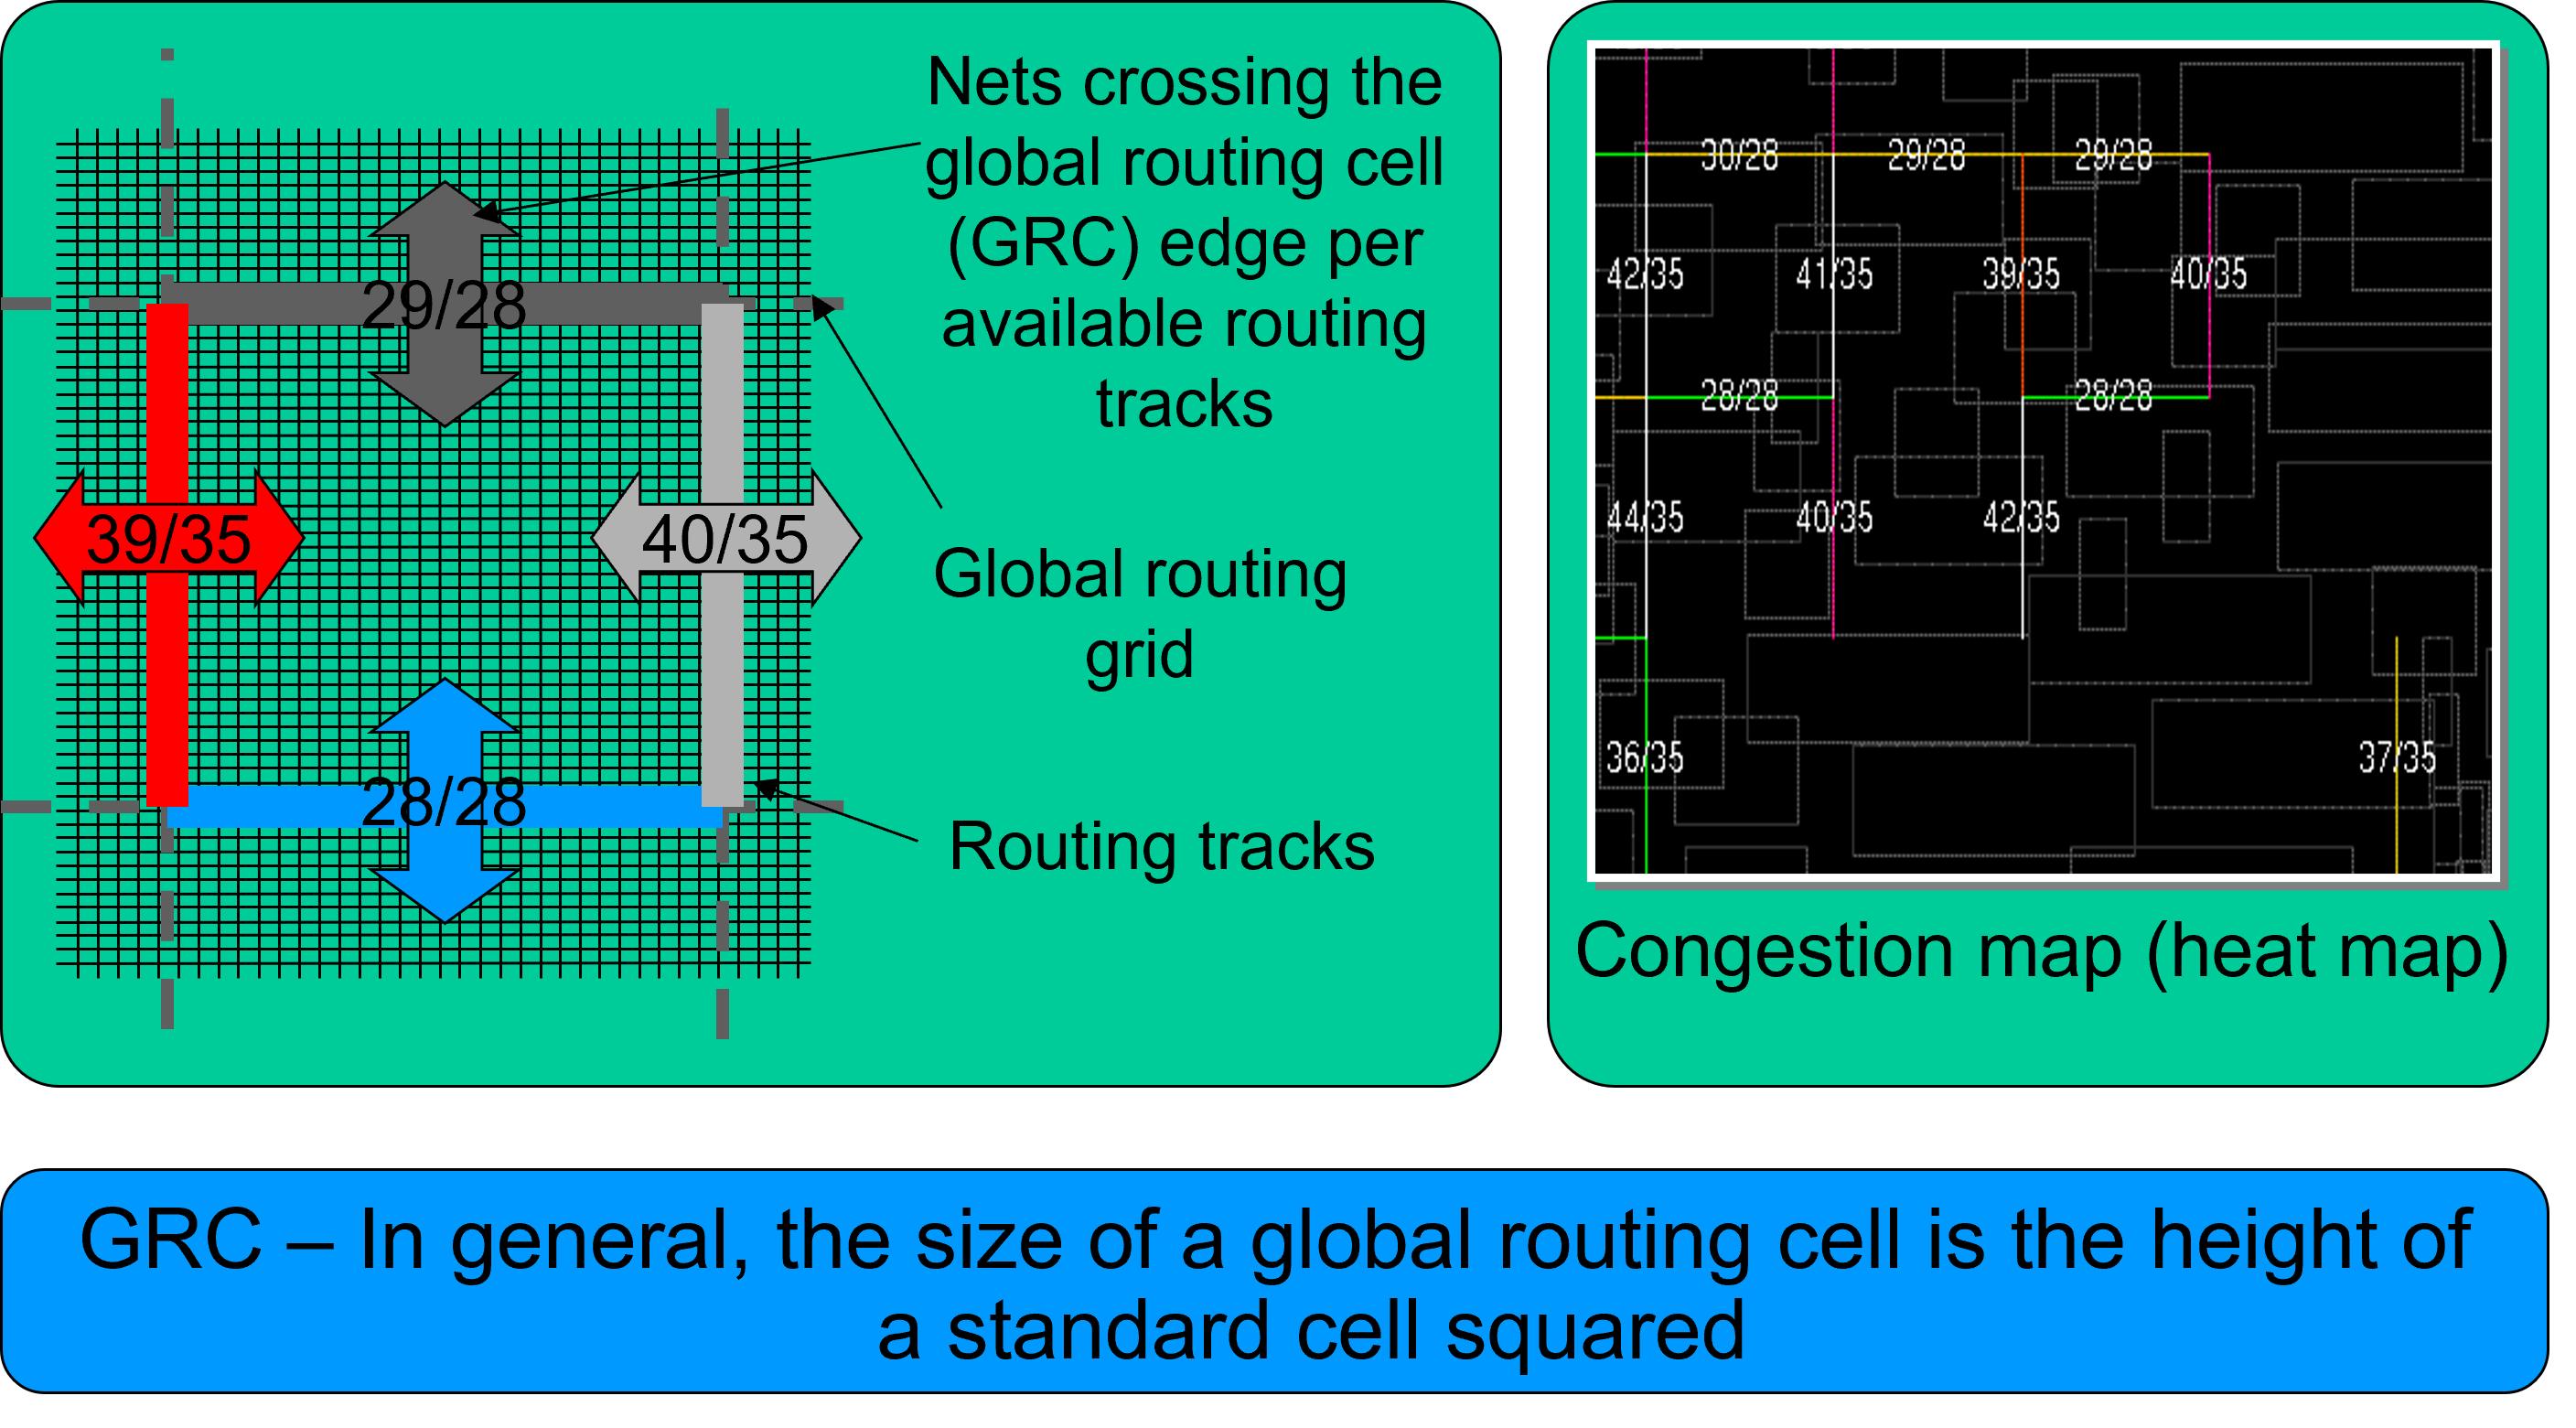
\includegraphics[width=\textwidth]{CDP2}
	\end{center}
\end{frame}

\begin{frame}
	\frametitle{Congestion-driven Placement}
		\begin{columns}
		\column{0.6 \textwidth}
		\begin{itemize}
			\item It is important to minimize or eliminate congestion before continuing
			
			\item Severe congestion can cause a design to be un-routable
			
		\end{itemize}
		\column{0.5 \textwidth}
		\begin{center}
			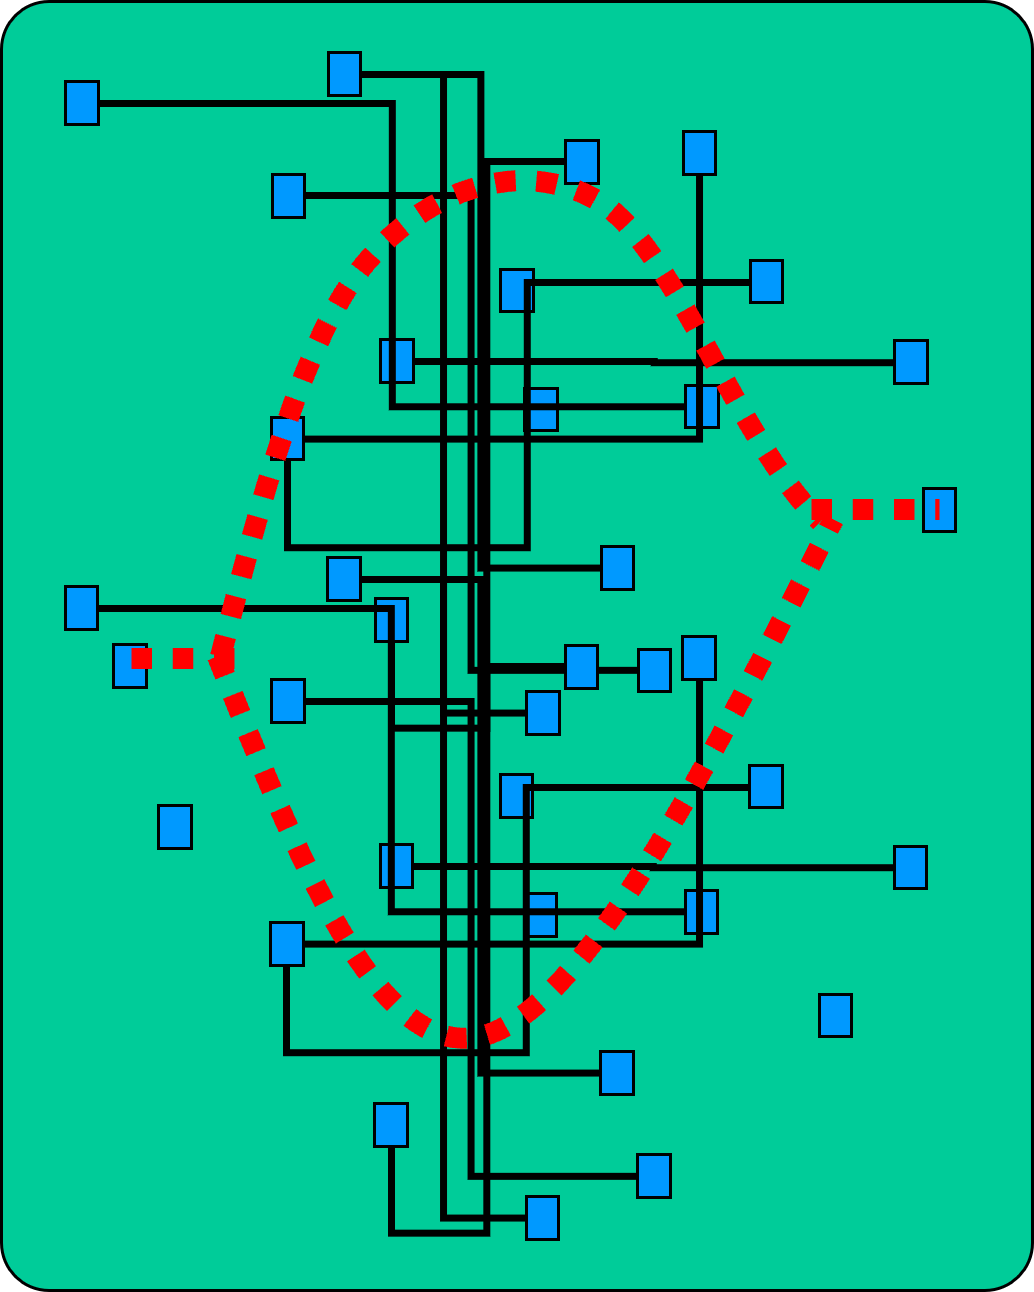
\includegraphics[width=0.8 \textwidth]{un-routable}
		\end{center}
	\end{columns}
\end{frame}

\subsection[Solution]{Congestion Reduction}
\begin{frame}
	\frametitle{Congestion-driven Placement}

		\begin{itemize}
			\item Congestion Reduction
			\begin{itemize}
				\item The tool tries to evaluate congestion hotspots
				and spread the cells (lower utilization) in the
				area to reduce congestion.
				\item The tool can also choose cell location based
				on congestion, rather than wire-length.
			\end{itemize}
			
		\end{itemize}
	
		\begin{center}
			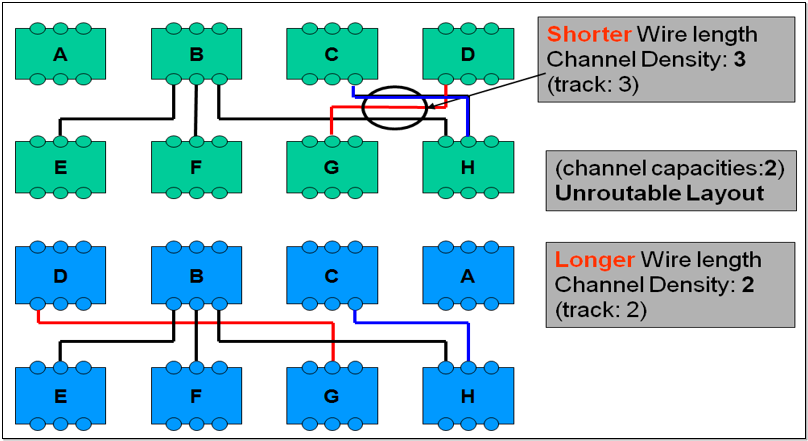
\includegraphics[width=0.8 \textwidth]{CDP3}
		\end{center}

\end{frame}

\begin{frame}
	\frametitle{Congestion vs. Timing-Driven Placement}
	\begin{center}
		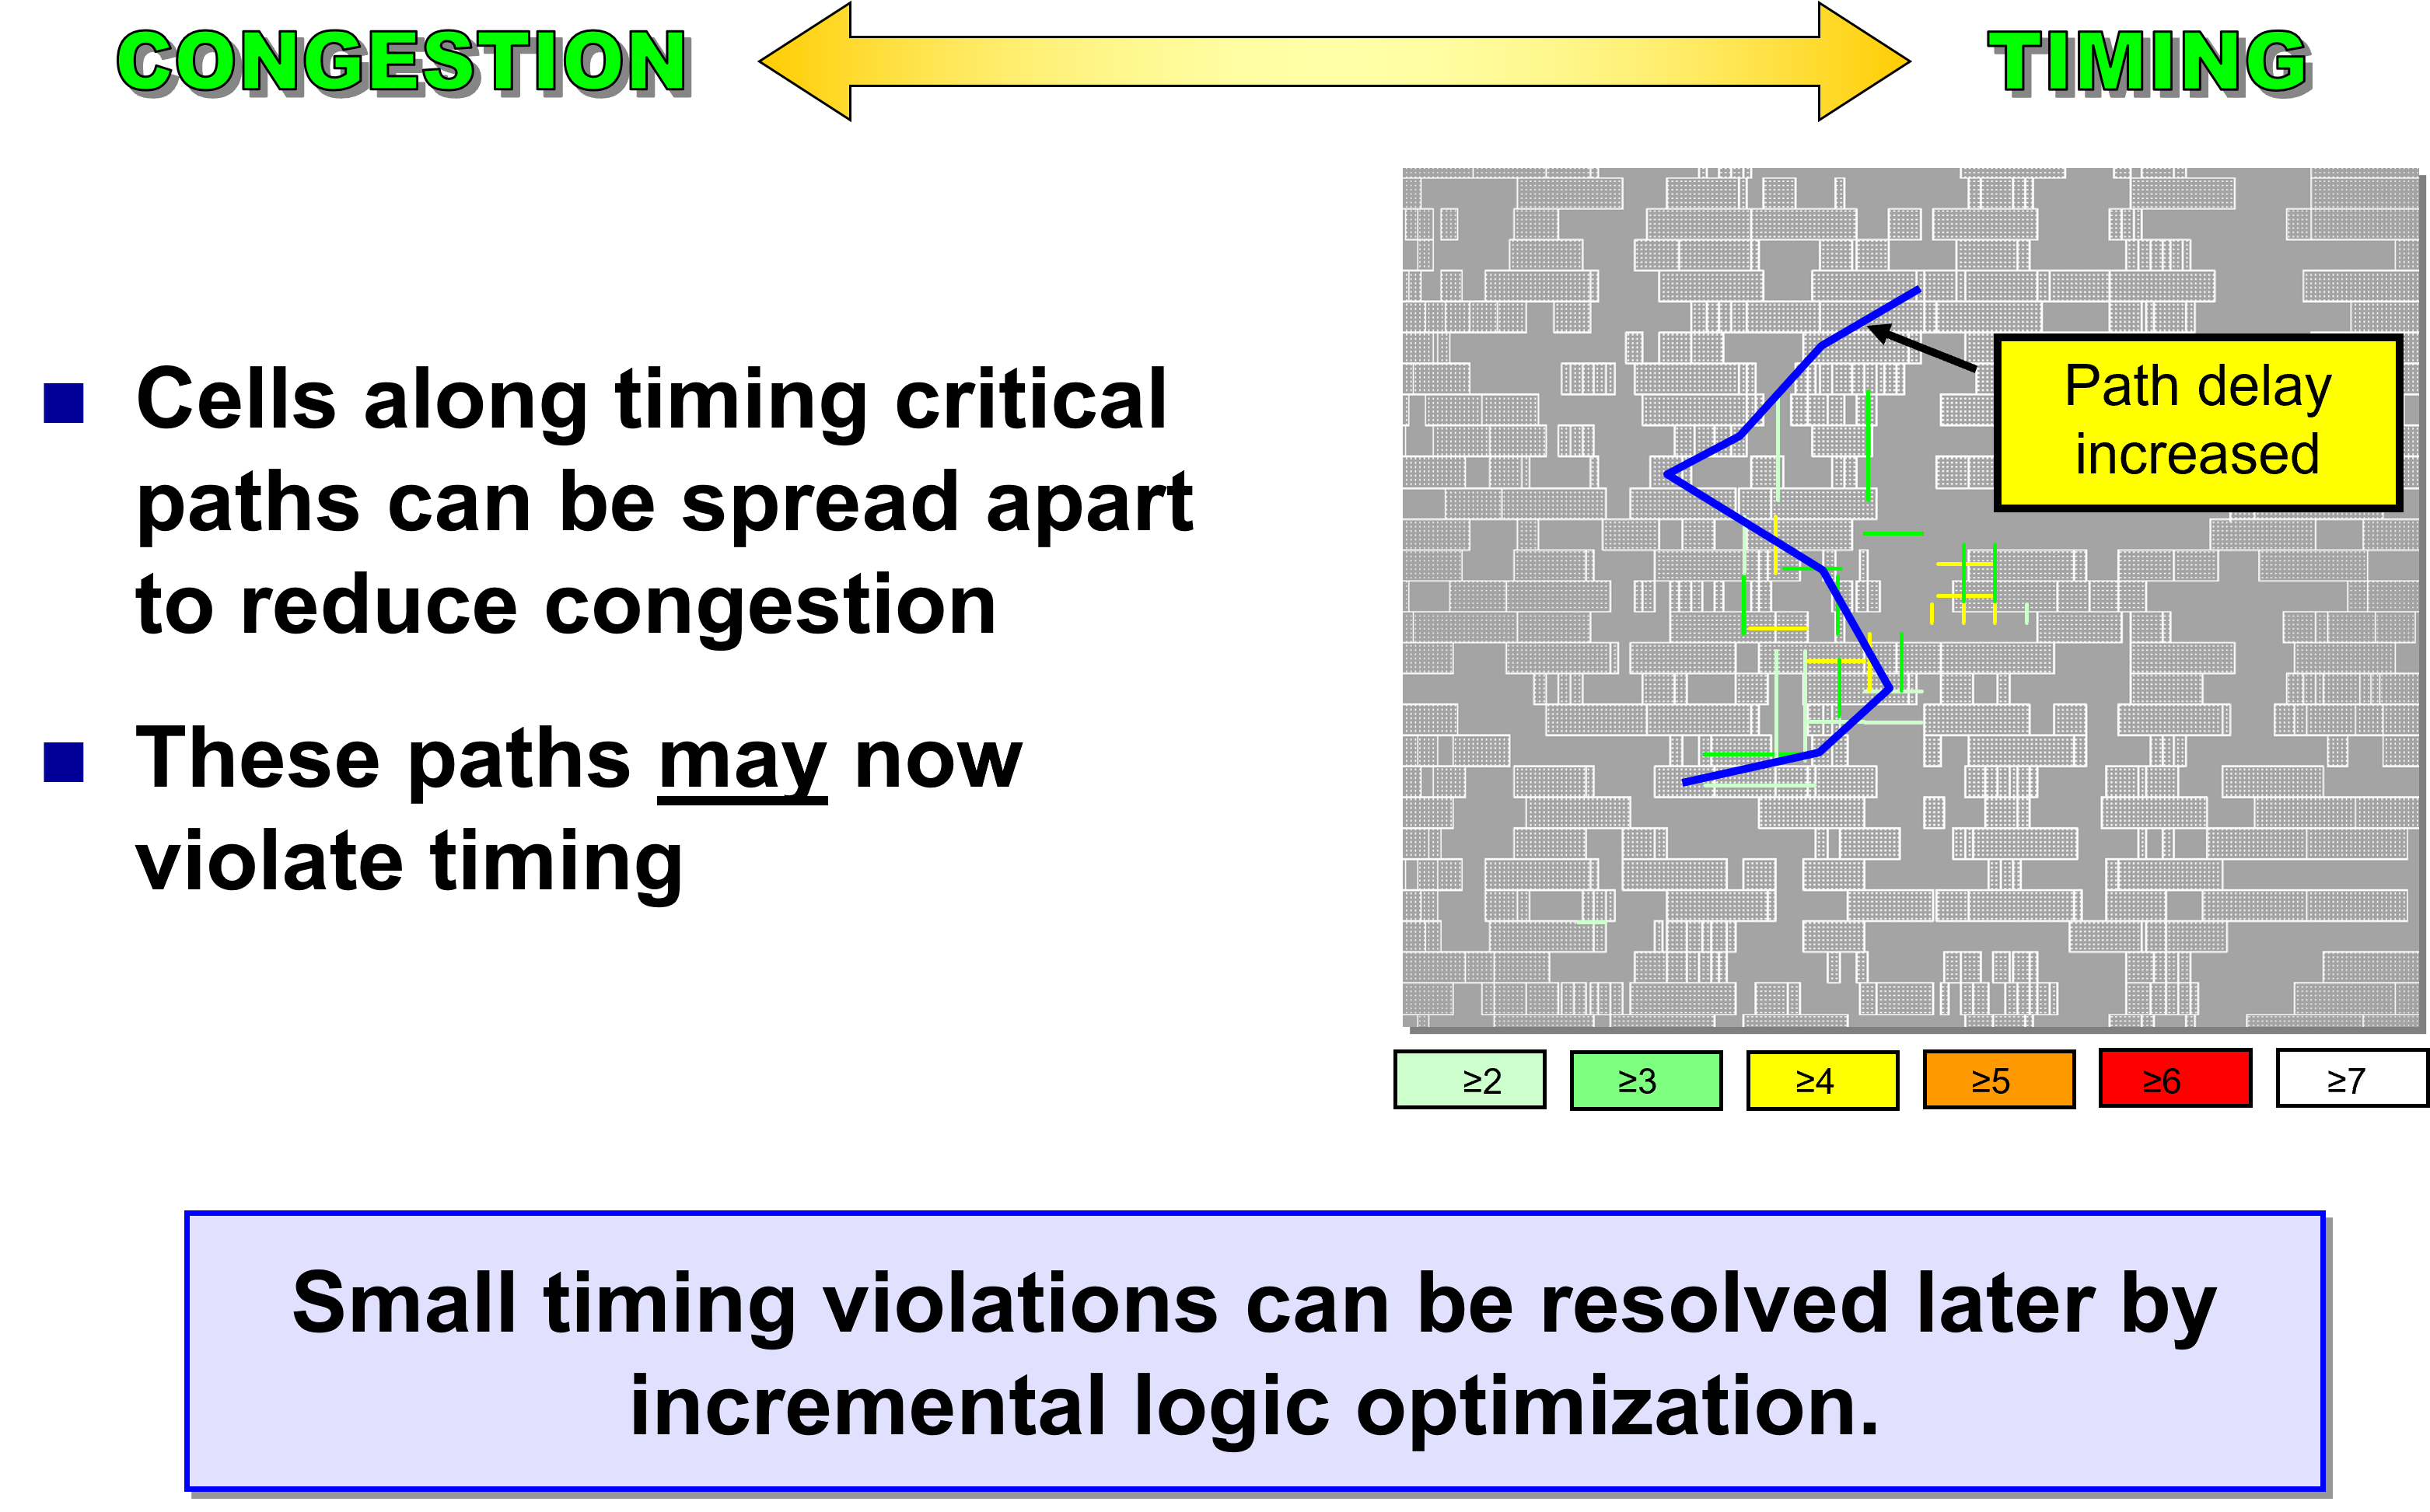
\includegraphics[width=\textwidth]{CvT}
	\end{center}
\end{frame}
\begin{frame}
	\frametitle{Global Route (GR) for Congestion Map}
	\begin{center}
		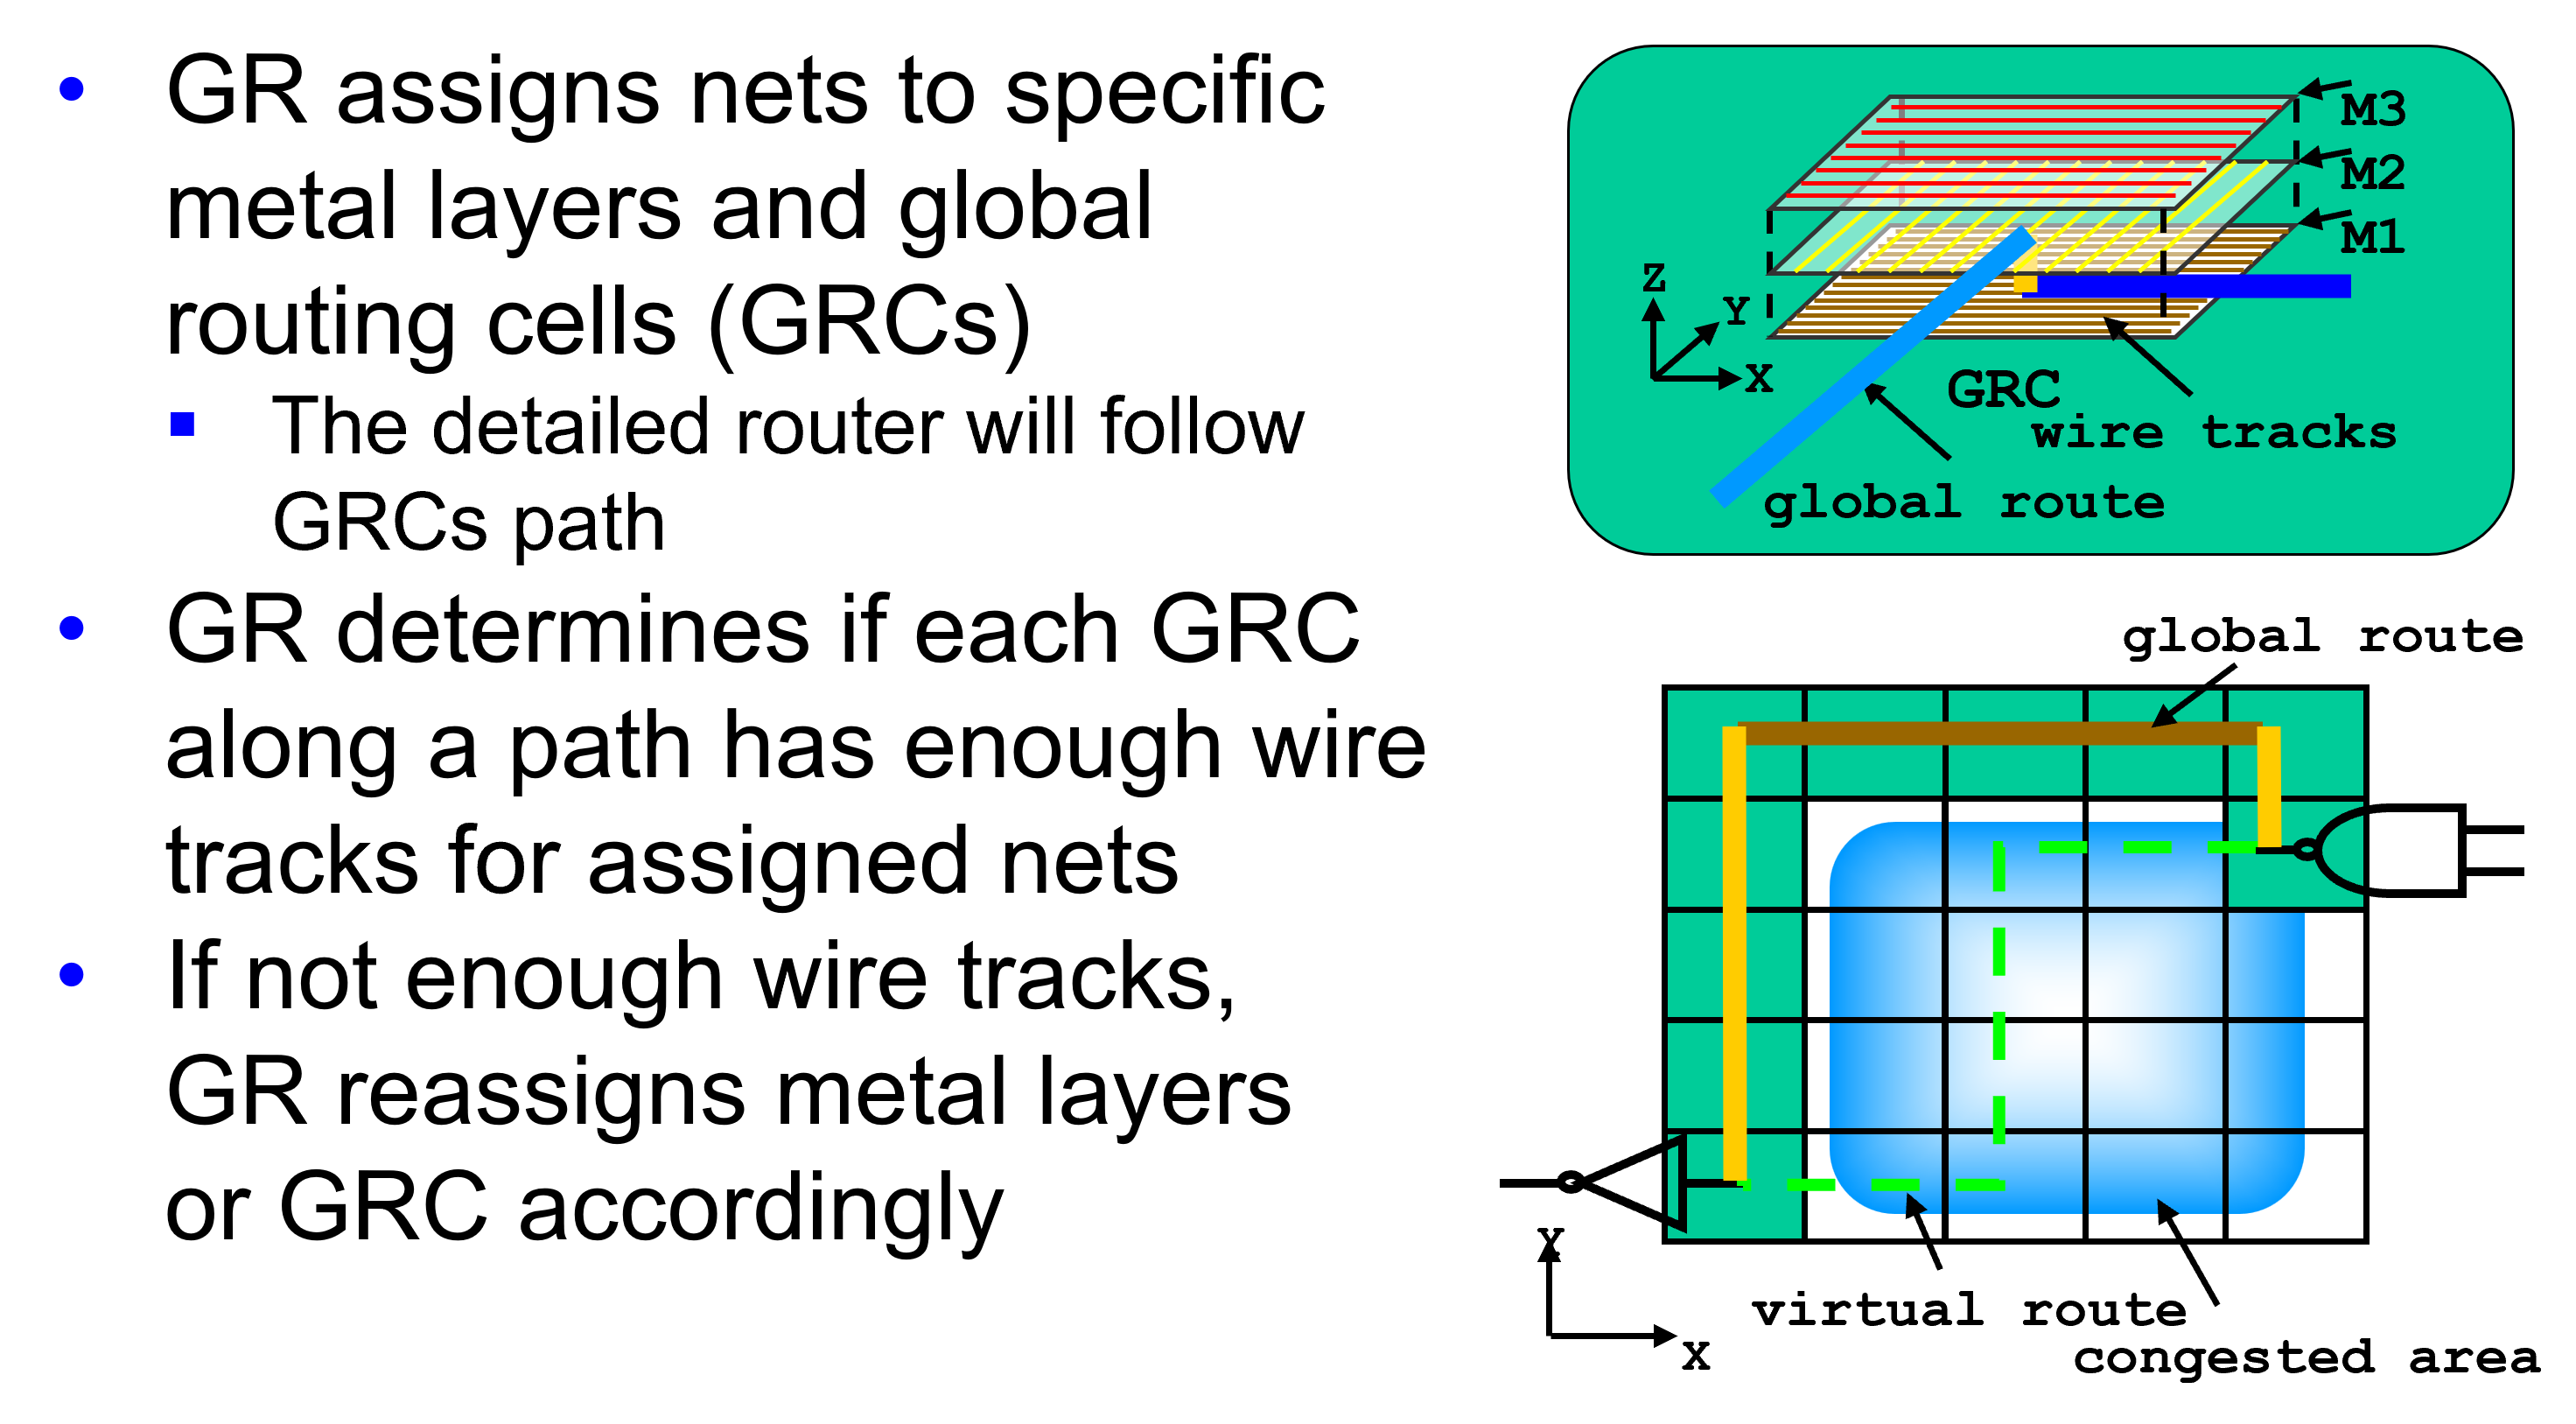
\includegraphics[width=\textwidth]{gr}
	\end{center}
\end{frame}

\begin{frame}
	\frametitle{Strategies to Fix Congestion}
	Modify the floorplan:
	\begin{itemize}
		\item Mark areas for low utilization.
		\item Top-level ports
			 \begin{itemize}
			\item Changing to a different metal layer
			\item Spreading them out, re-ordering or moving to other sides
		\end{itemize}
		\item Macro location or orientation
		\begin{itemize}
			\item Alignment of bus signal pins
			\item Increase of spacing between macros
			\item Add blockages and halos
		\end{itemize}
		\item Core aspect ratio and size
			 \begin{itemize}
			\item Making block taller to add more horizontal routing resources
			\item Increase of the block size to reduce overall congestion
		\end{itemize}
		\item Power grid
			 \begin{itemize}
			\item Fixing any routed or non-preferred layers
		\end{itemize}
	\end{itemize}

\end{frame}

\section[HFNS]{High Fanout Synthesis (HFS)}
\subsection[HFNS]{High Fanout Synthesis (HFS)}
\begin{frame}
	\frametitle{High Fanout Synthesis (HFS)}
	\begin{center}
		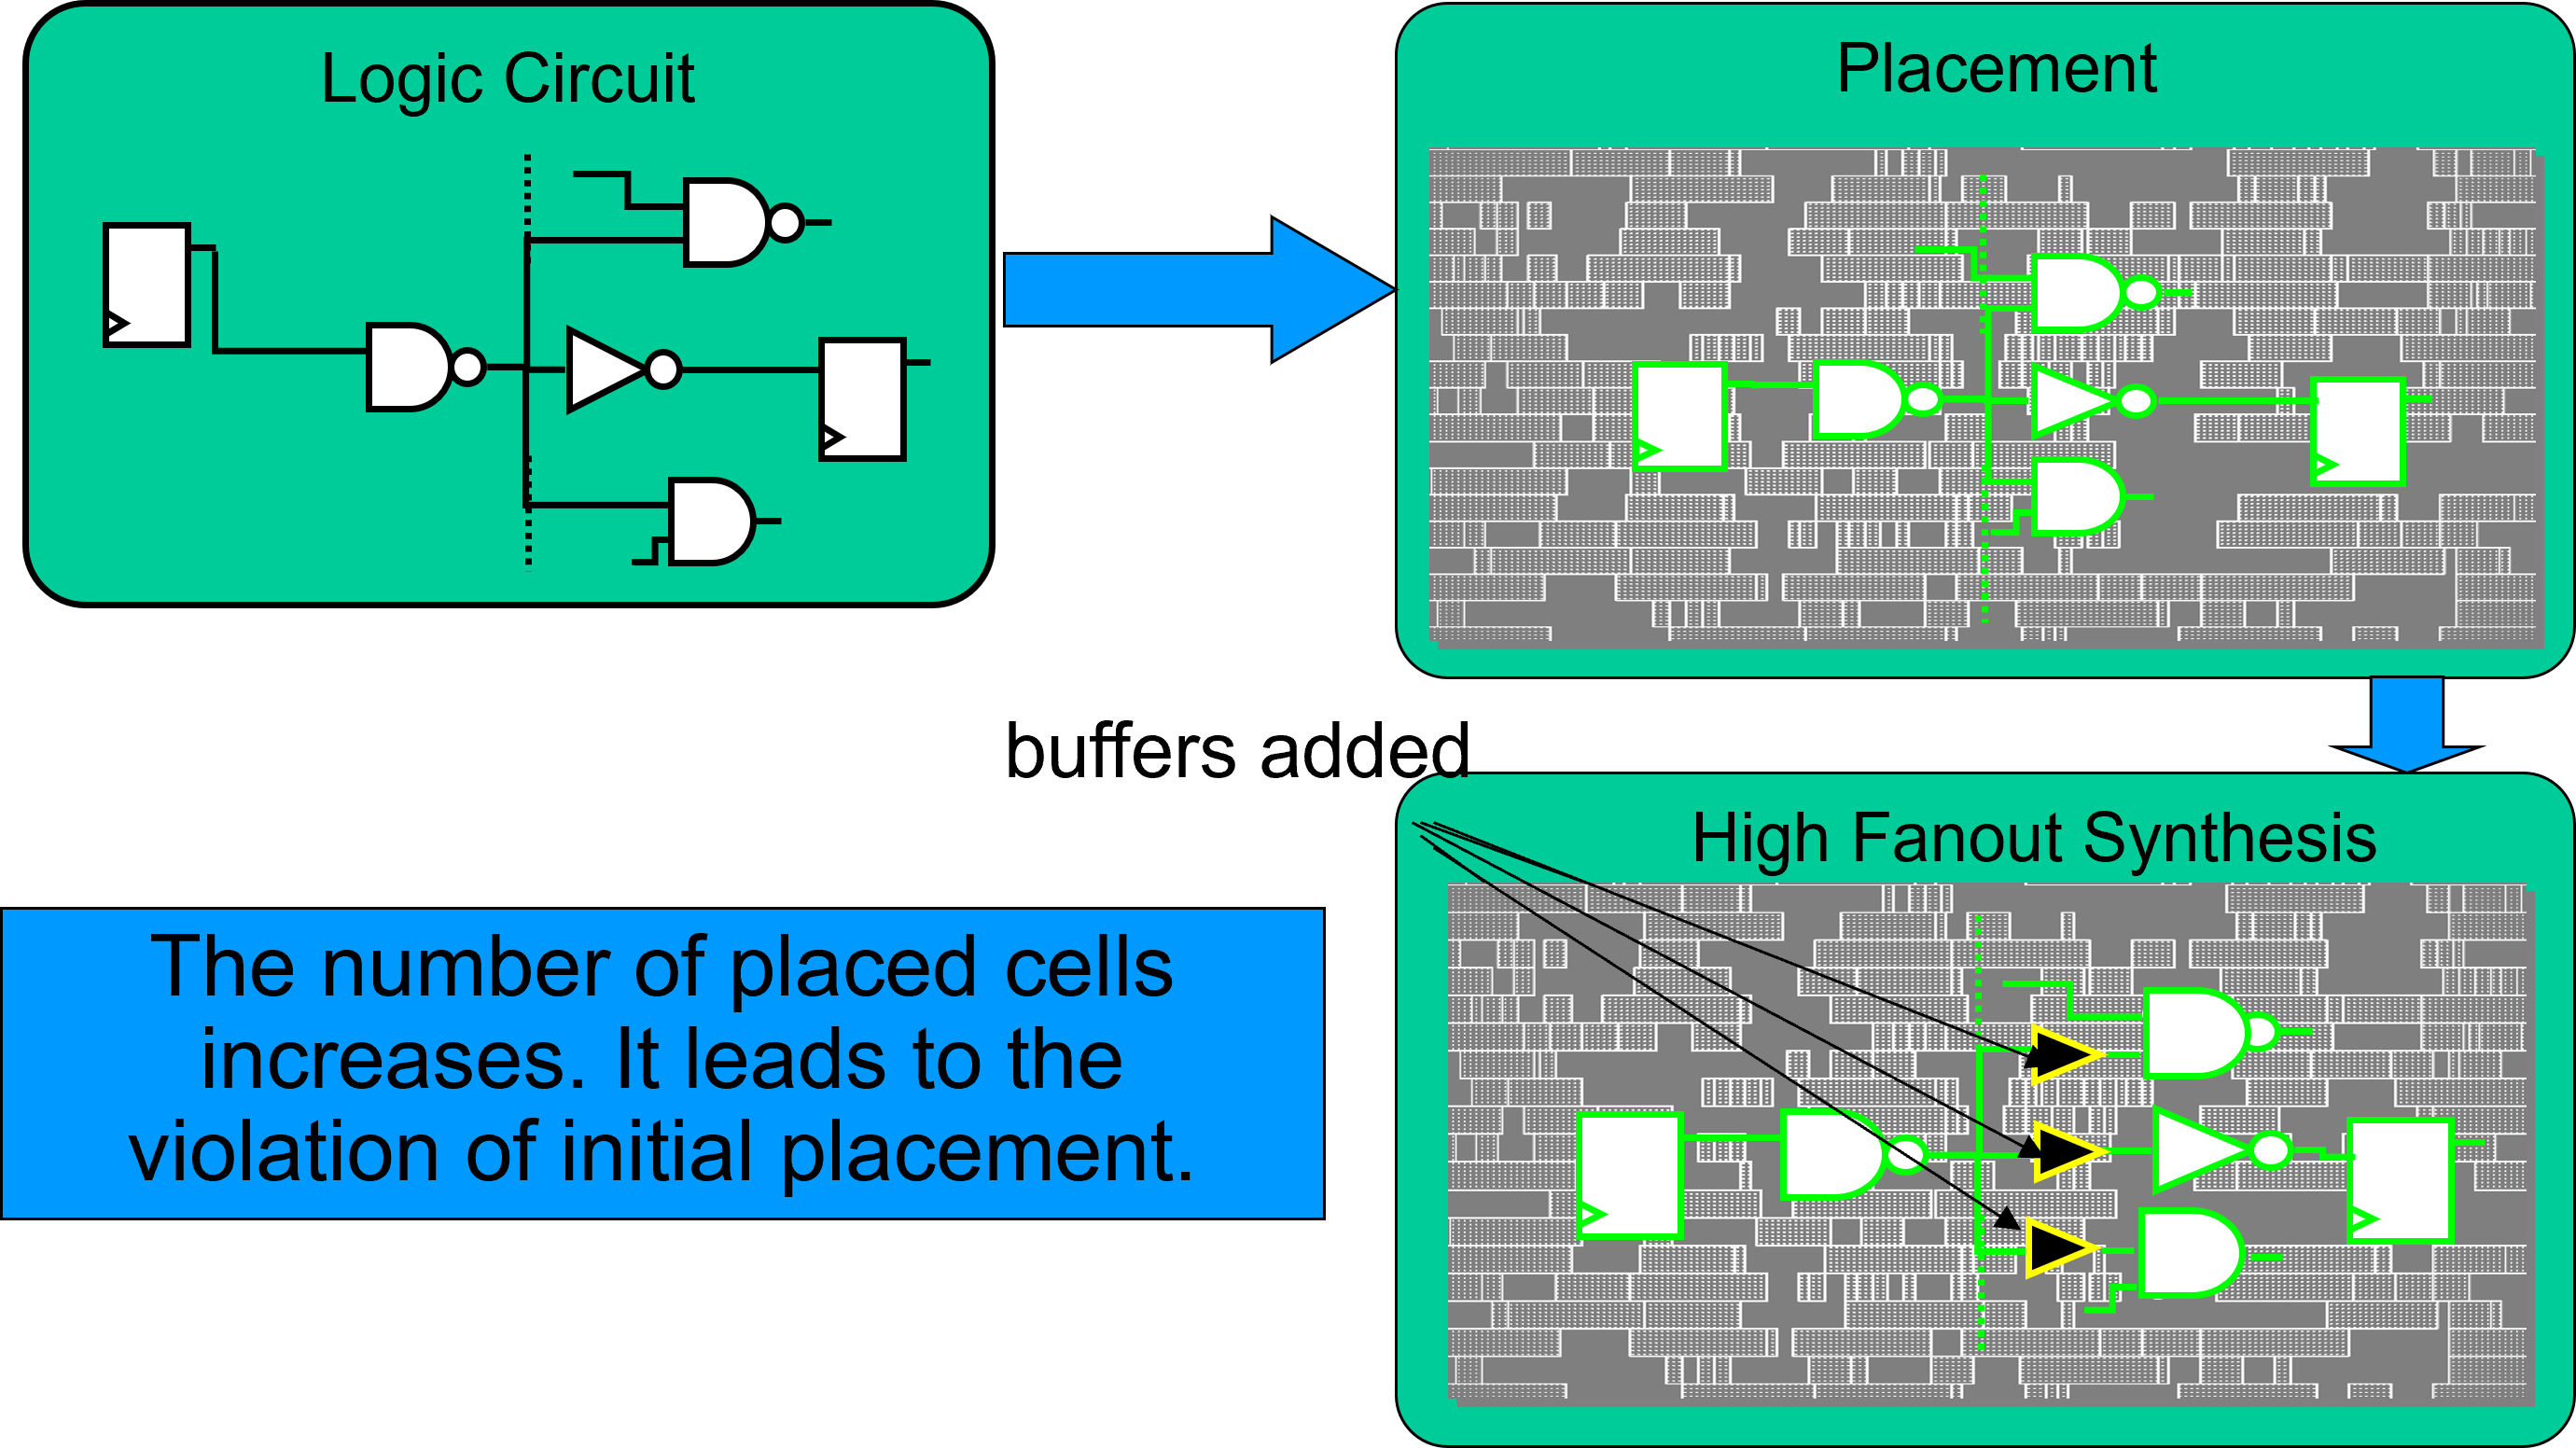
\includegraphics[width=\textwidth]{HFS}
	\end{center}
\end{frame}
\begin{frame}
	\frametitle{High Fanout Synthesis}
	\begin{itemize}
		\item \textbf{What is fanout?}
			\begin{itemize}
				\item Fanout is the number of gate inputs to which the output can be safely connected. i.e., The load that a gate output can drive. 
				\item The maximum fanout of an output measures it’s load-driving capability. Fanout belongs to the output.
			\end{itemize}
		\item \textbf{What are High Fanout Nets(HFN) ?}
		\begin{itemize}
			\item High Fanout Nets are the nets which drive more number of load. We set some max fanout limit by using the command \textcolor{red}{set\_max\_fanout}
			\item The nets which have greater than these limit are considered as High Fanout Nets (HFN). 
			\item Generally clock nets, reset, scan, enable nets are High Fanout Nets.
		\end{itemize}
	\end{itemize}
\end{frame}

\begin{frame}
	\frametitle{What is High Fanout Net Synthesis (HFNS)?}
	\begin{itemize}
		\item High Fanout Net Synthesis (HFNS) is the process of buffering the High Fanout Nets to balance the load.
		
		\item To balance the load HFNS is perfomed.
		\item Too many load affects delay numbers and transition times, Because load is directly proportional to the delay.
		\item Generally at placement step HFNS performed. HFNS can also be performed at synthesis step using Design Compiler. But it’s not good idea, Buffers will be removed during PD and again HFNS is performed.
		\item \textbf{Care that should taken during HFNS:}
	\begin{enumerate}
		\item Make sure an appropriate fanout limit is set using \textcolor{red}{set\_max\_fanout} command
		\item Verify the SDC used for PD should not have \textcolor{red}{set\_ideal\_network} or \textcolor{red}{set\_dont\_touch} commands on High Fanout Nets.
		\item Use ideal clock network – As clock nets are synthesized separately during Clock Tree Synthesis (CTS) step, we set clock network as ideal network.
		
	\end{enumerate}
		
	\end{itemize}
\end{frame}

\section[Scan Chain]{Scan Chain Reordering}
\subsection[Scan Chain]{Scan Chain}
\begin{frame}
	\frametitle{Pre-Existing Scan Chains?}
	\begin{center}
		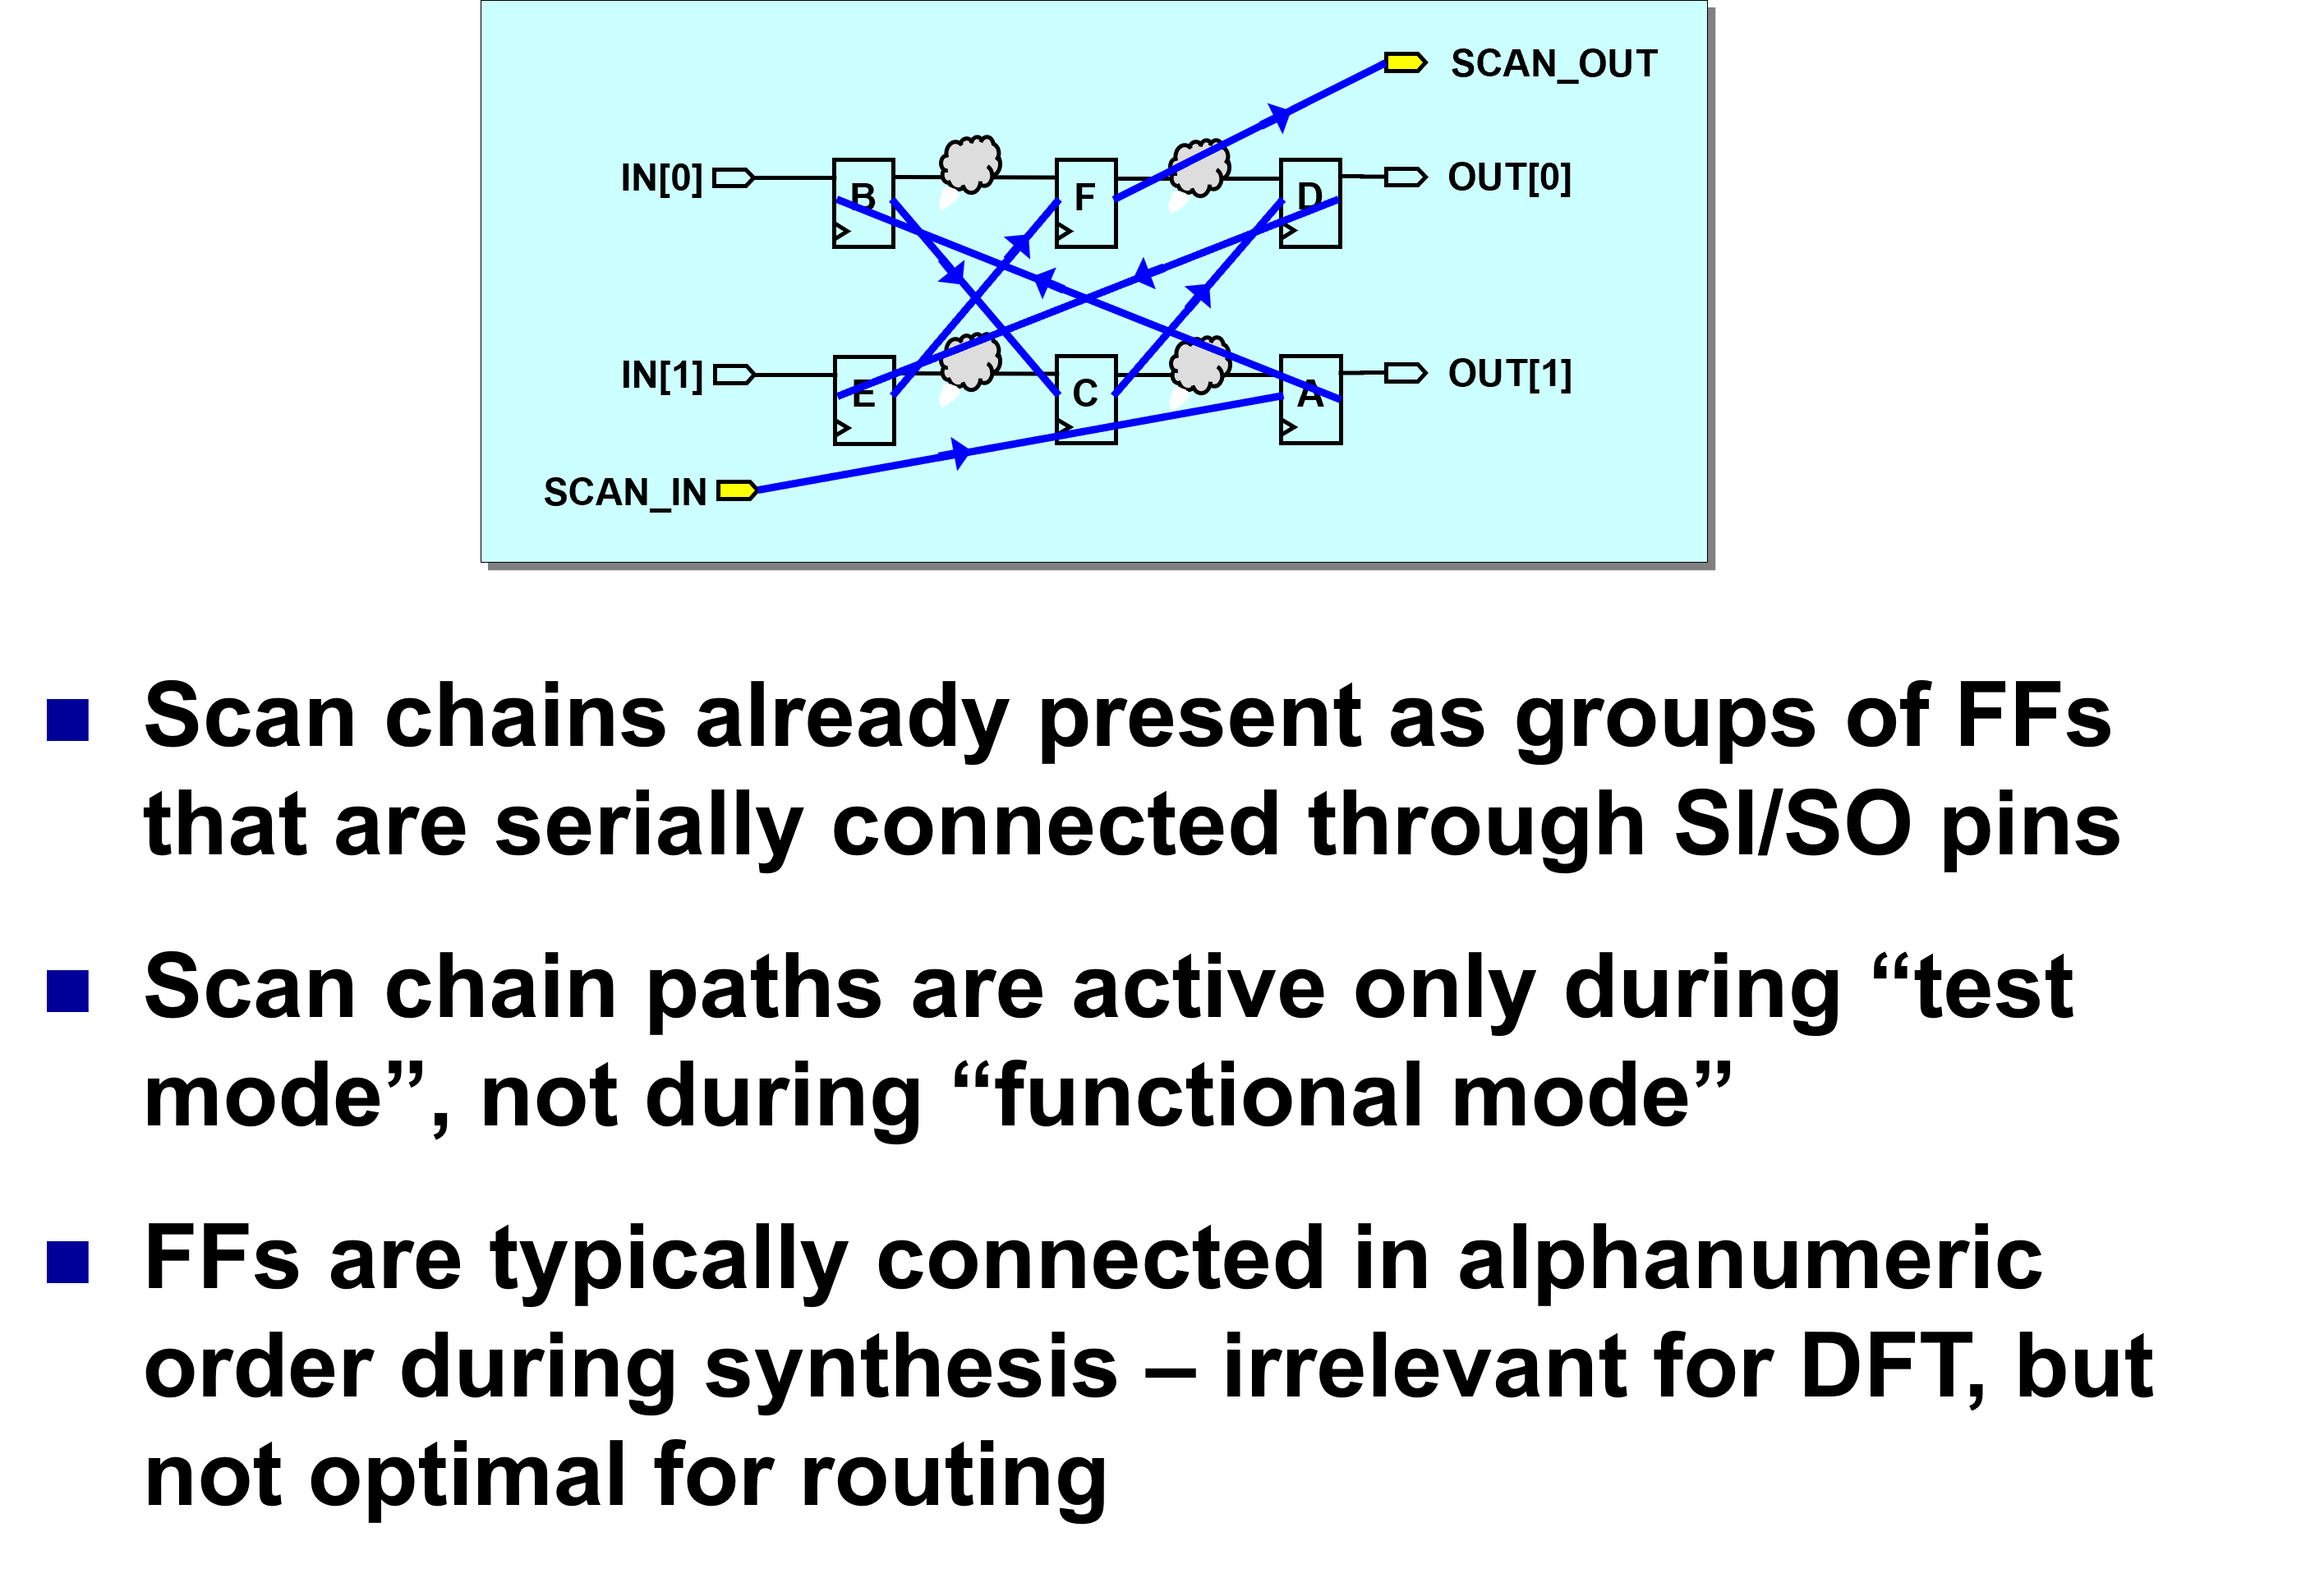
\includegraphics[width=\textwidth]{SC}
	\end{center}
\end{frame}

\begin{frame}
	\frametitle{What’s the Issue with Existing Scan Chains?}
	\begin{center}
		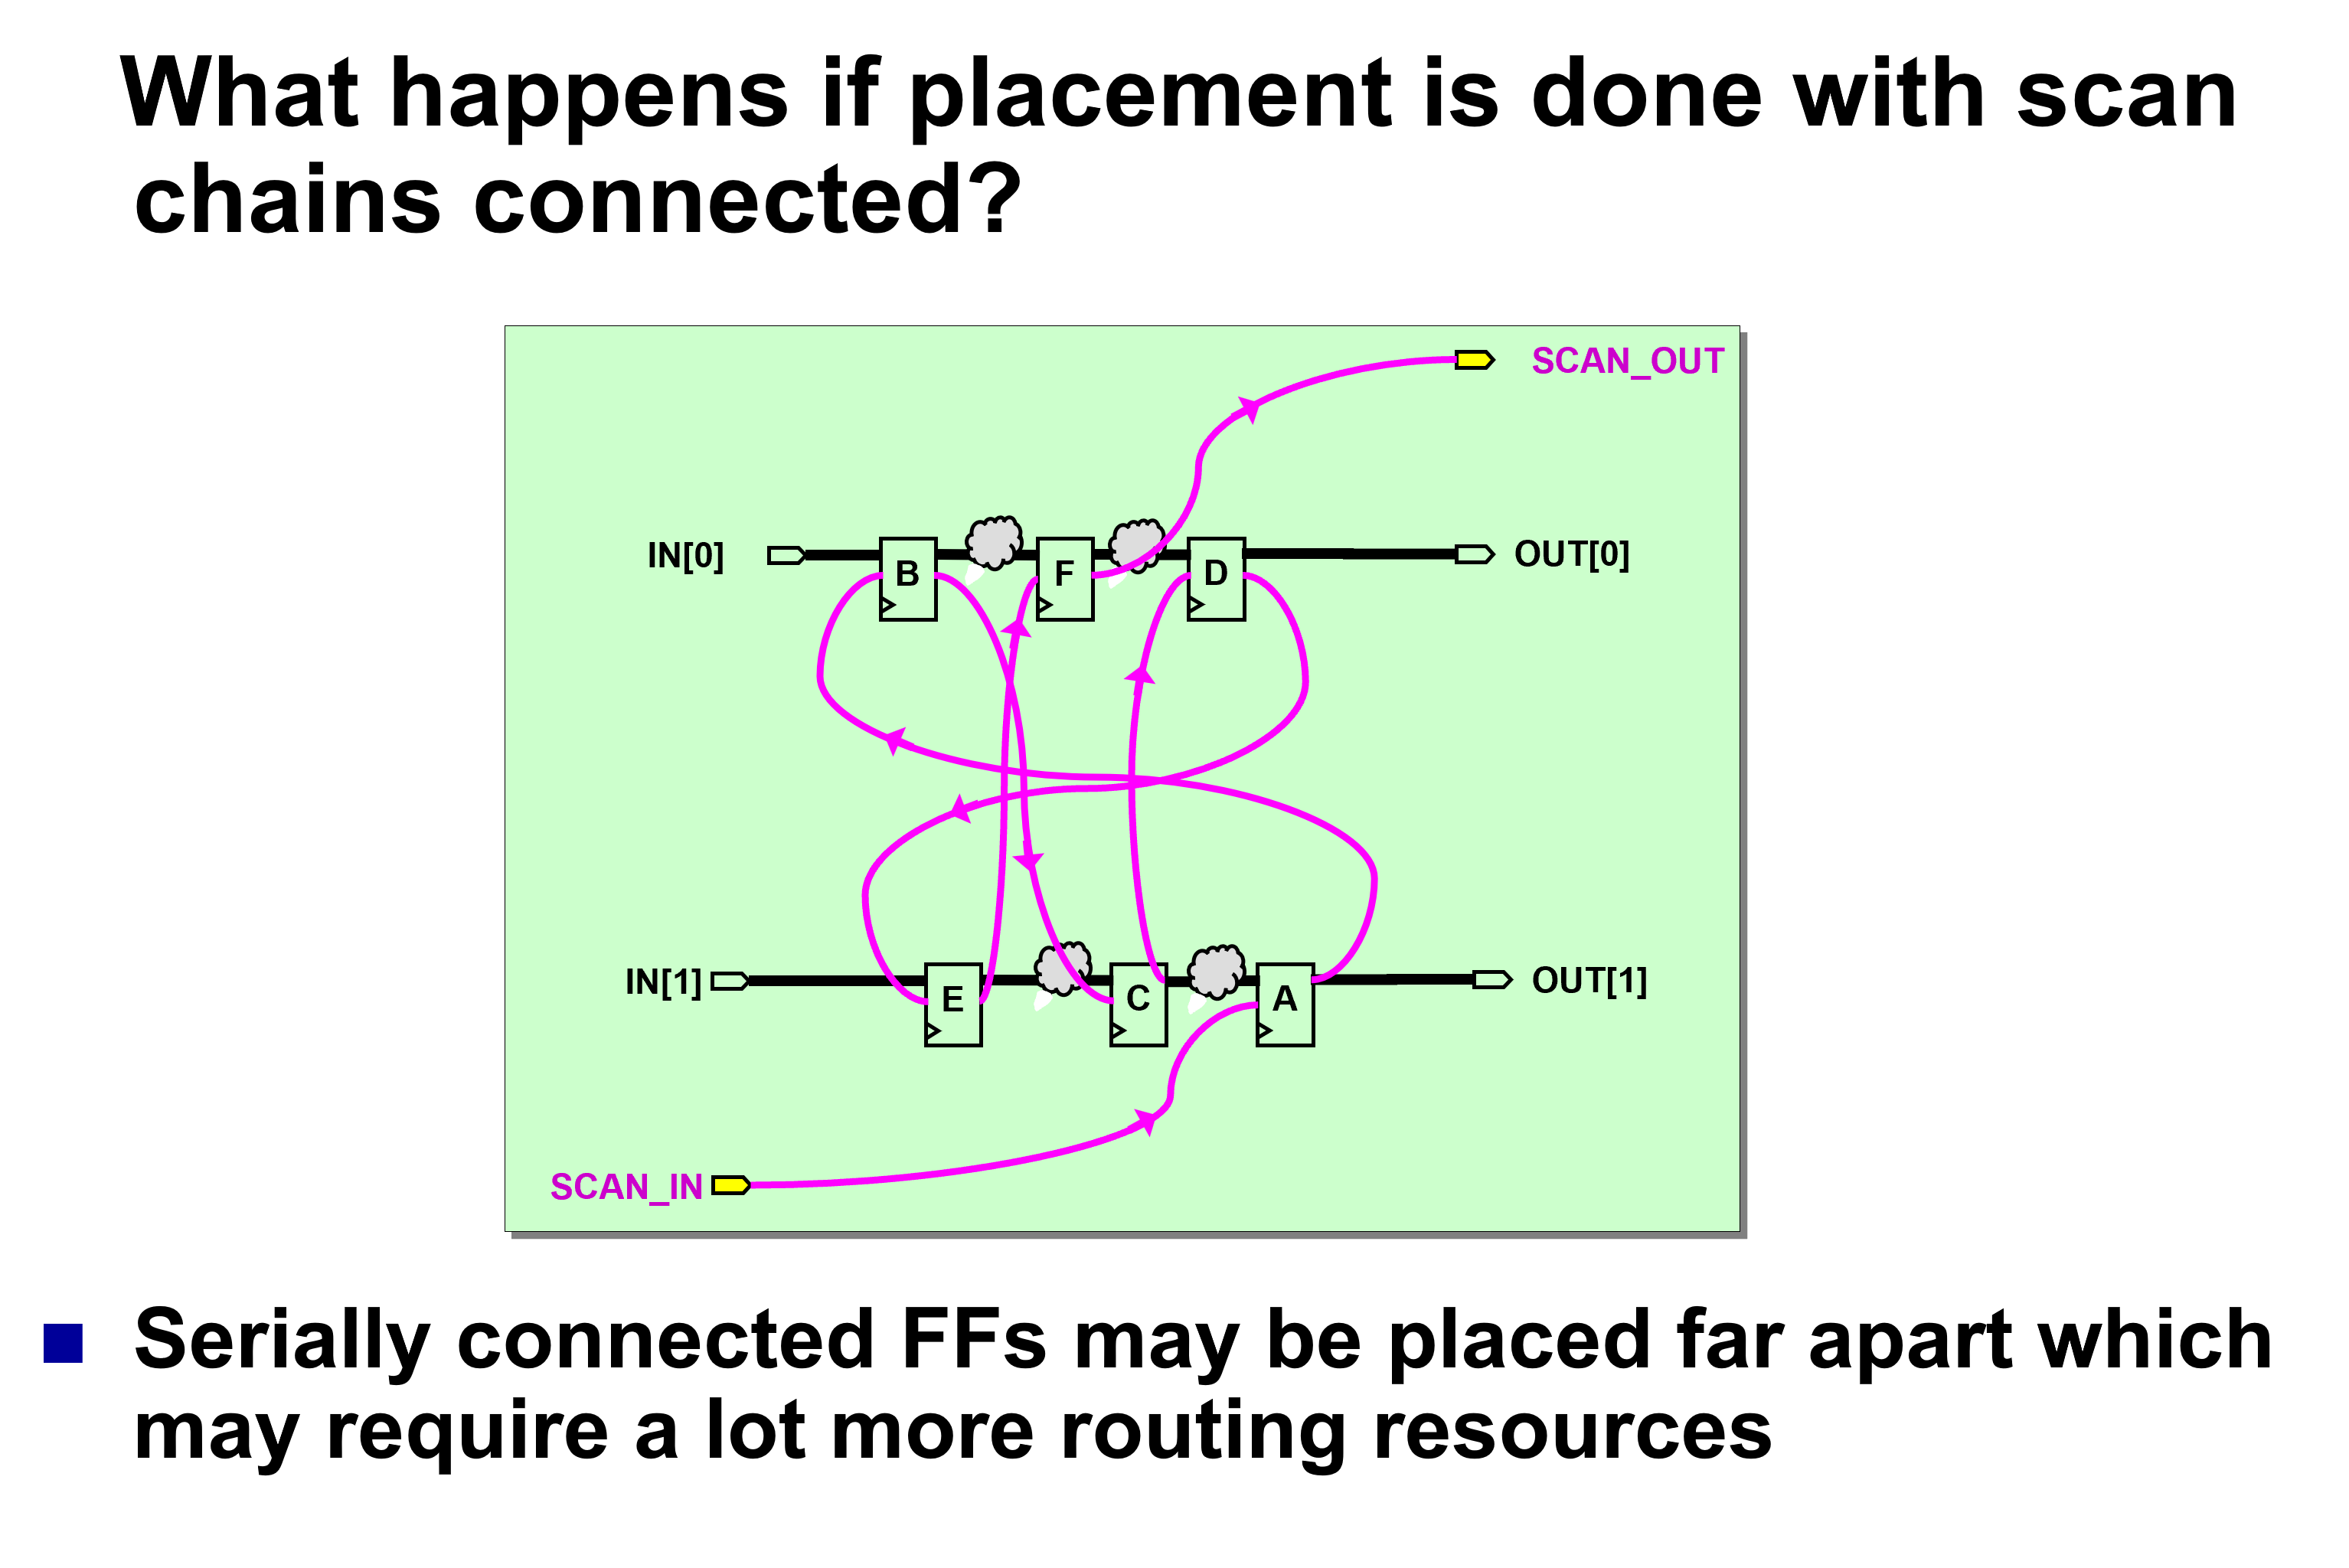
\includegraphics[width=\textwidth]{SC1}
	\end{center}
\end{frame}

\begin{frame}
	\frametitle{Placement Based Scan Chain Routing}
	\begin{center}
		\includegraphics[width=\textwidth]{SC2}
	\end{center}
\end{frame}
\begin{frame}
	\frametitle{SCANDEF Reordering}
		\begin{center}
		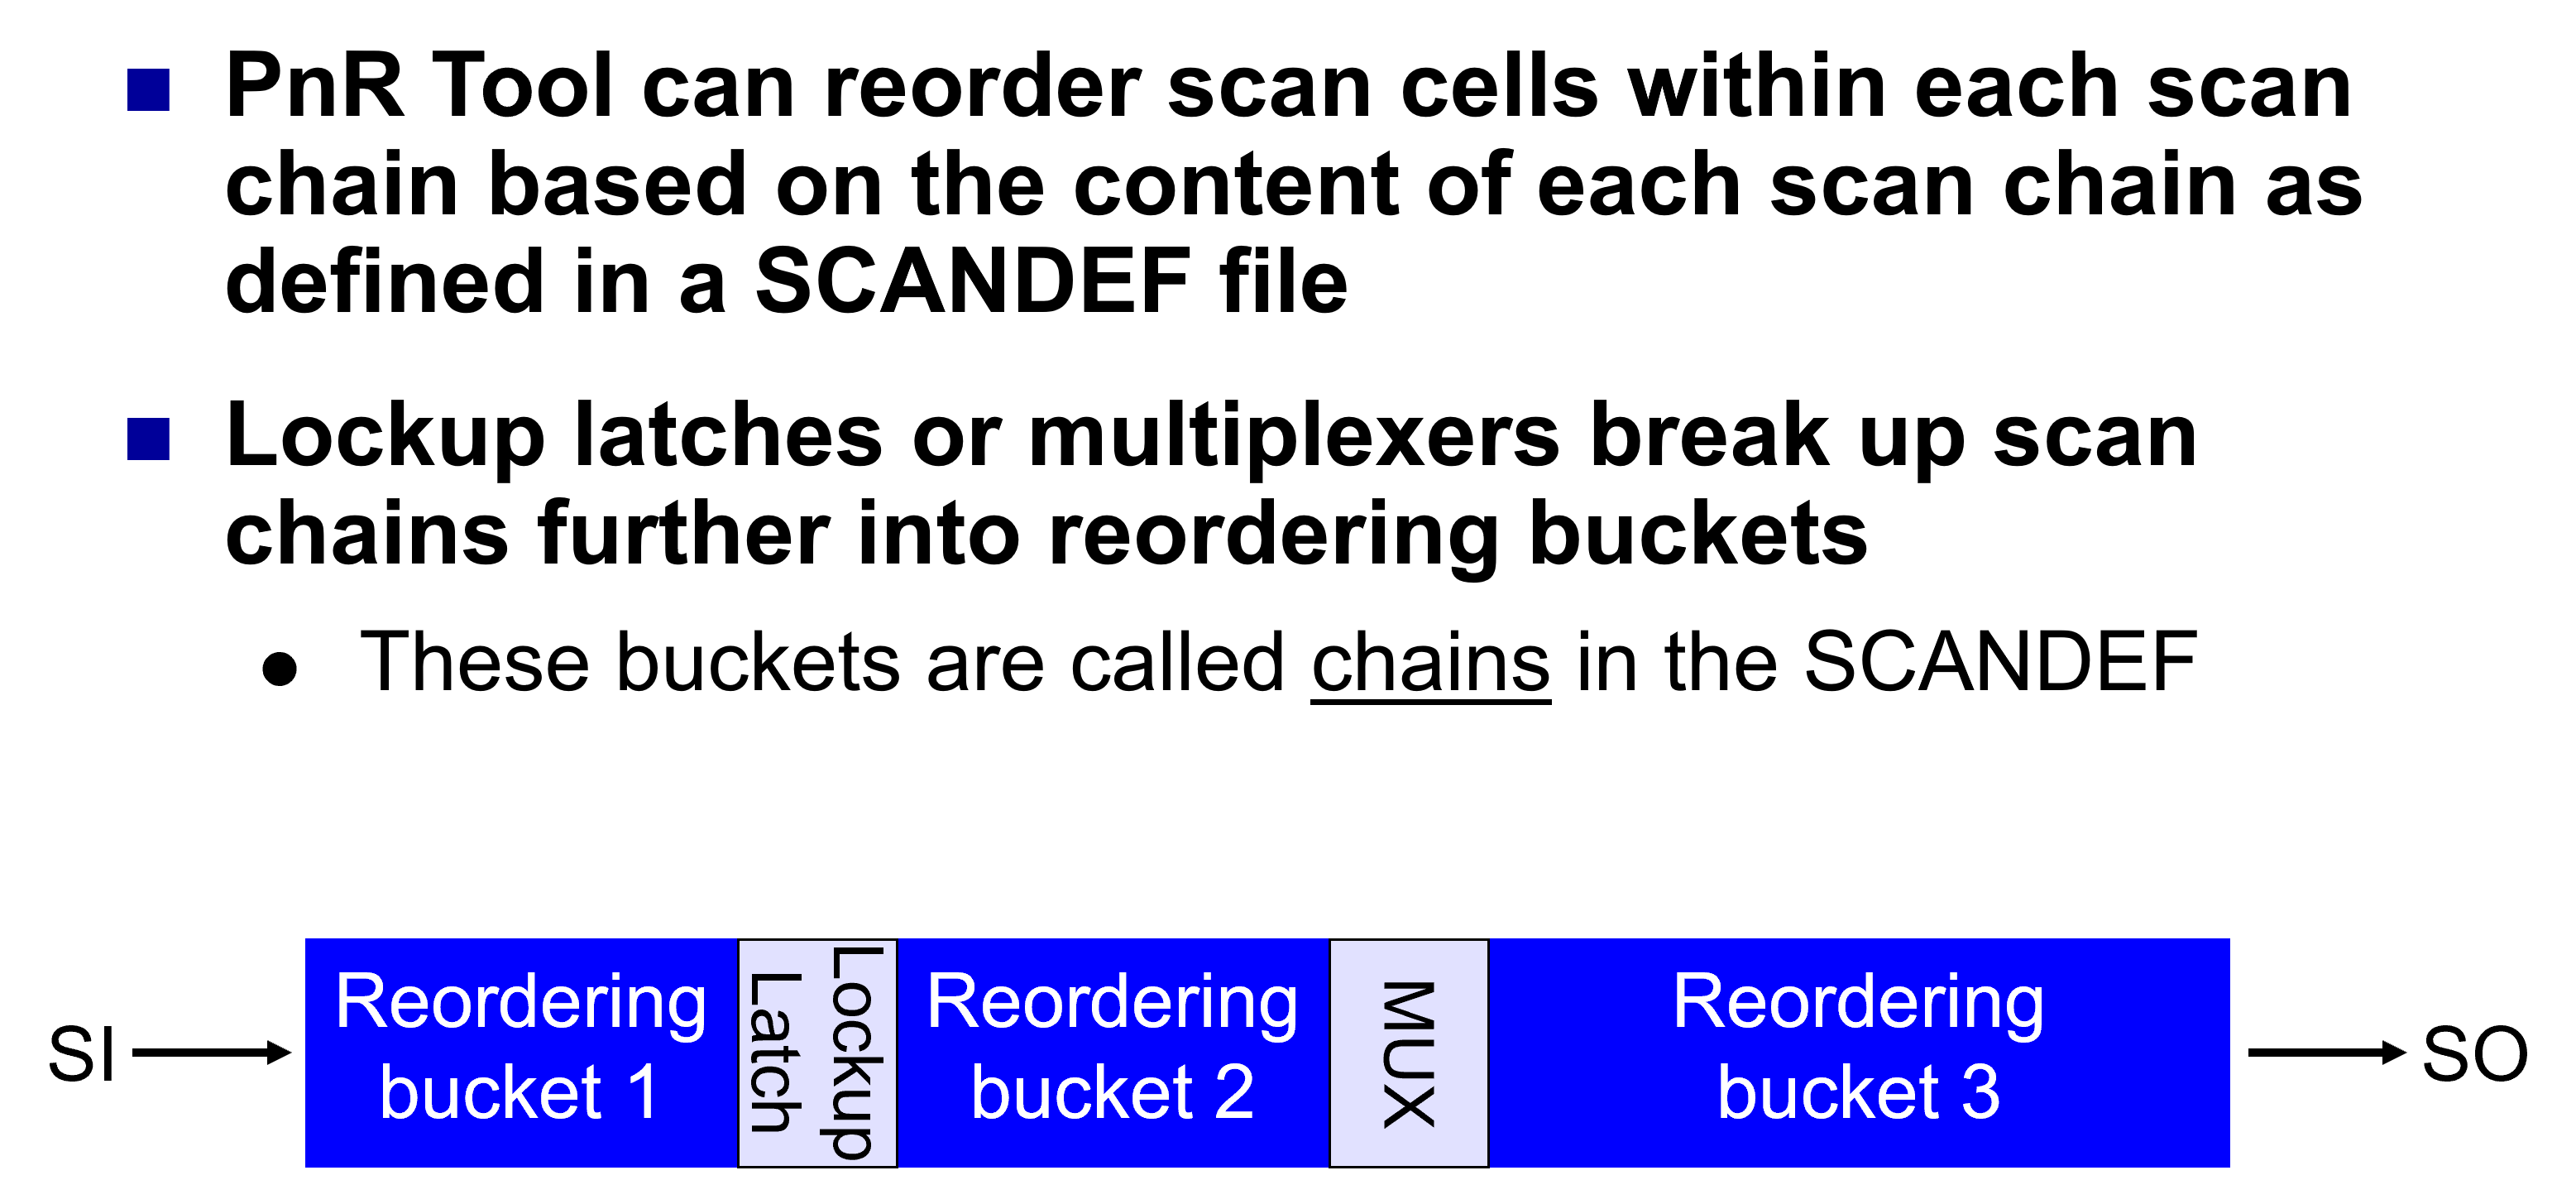
\includegraphics[width=\textwidth]{SC3}
	\end{center}
\end{frame}

\begin{frame}
	\frametitle{Partitioning with SCANDEF}
	\begin{center}
		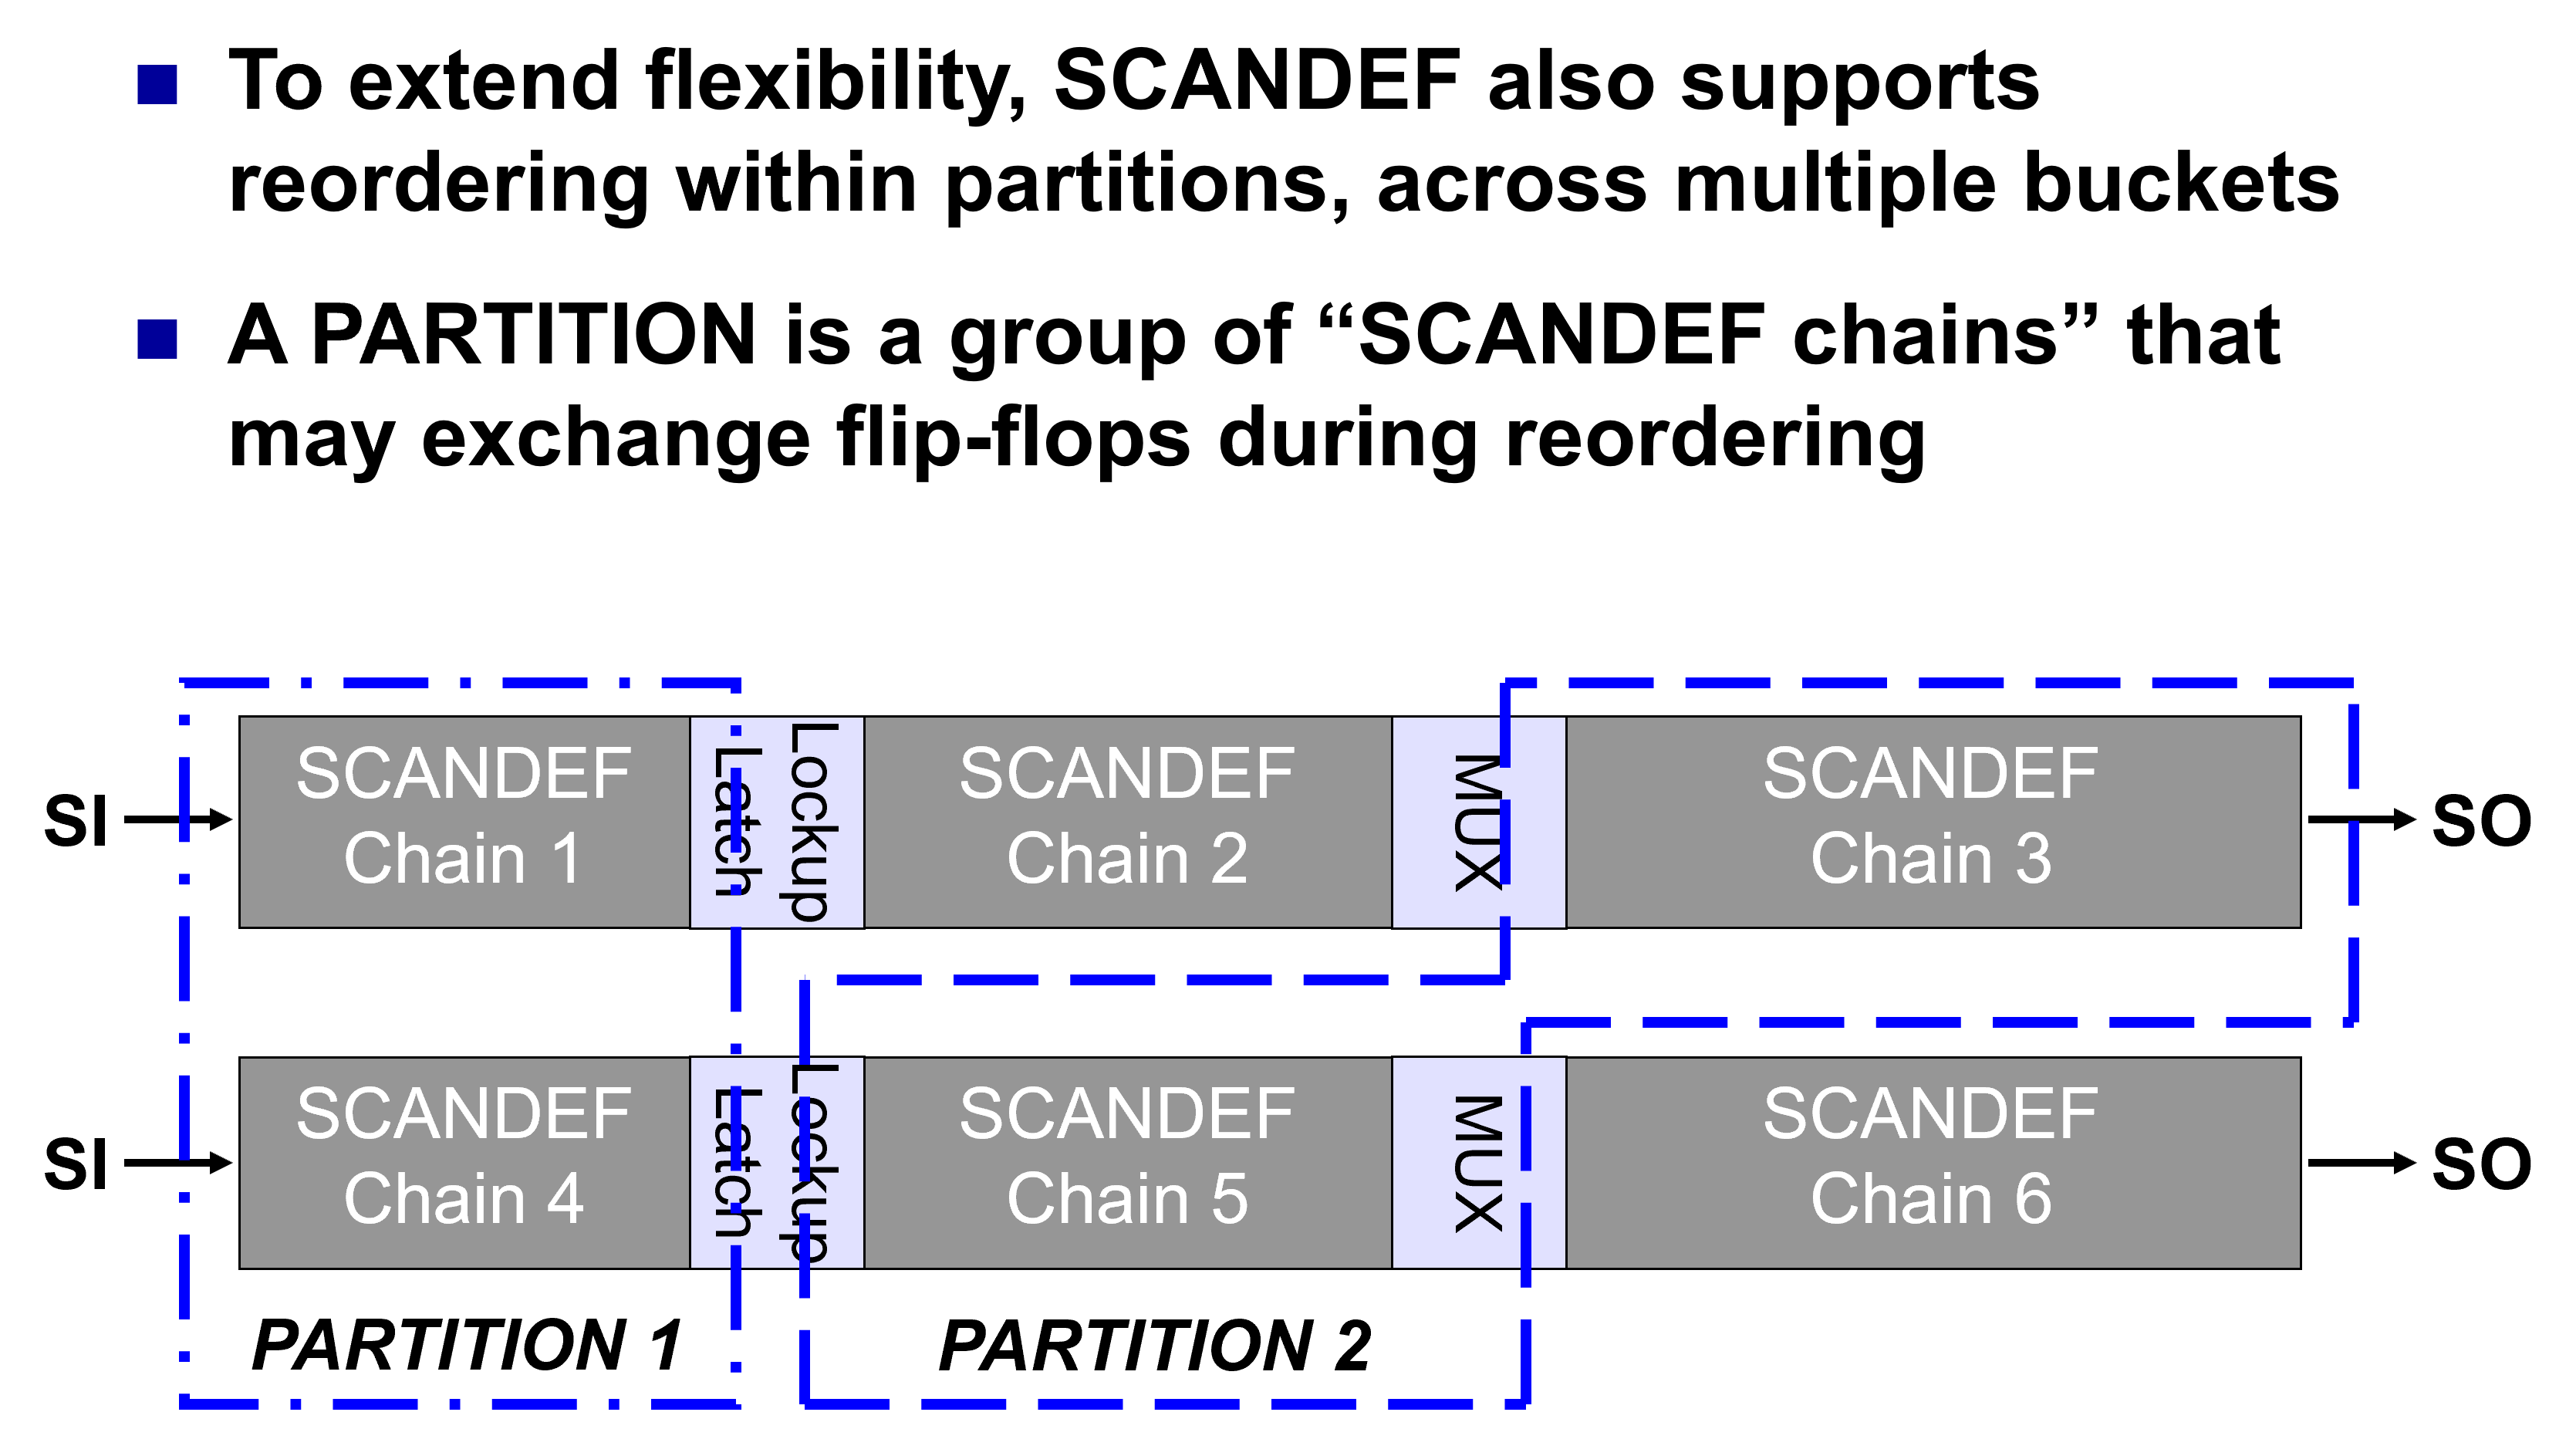
\includegraphics[width=\textwidth]{SC4}
	\end{center}
\end{frame}

\begin{frame}
	\frametitle{SCANDEF generated with DFTC}
	\begin{center}
		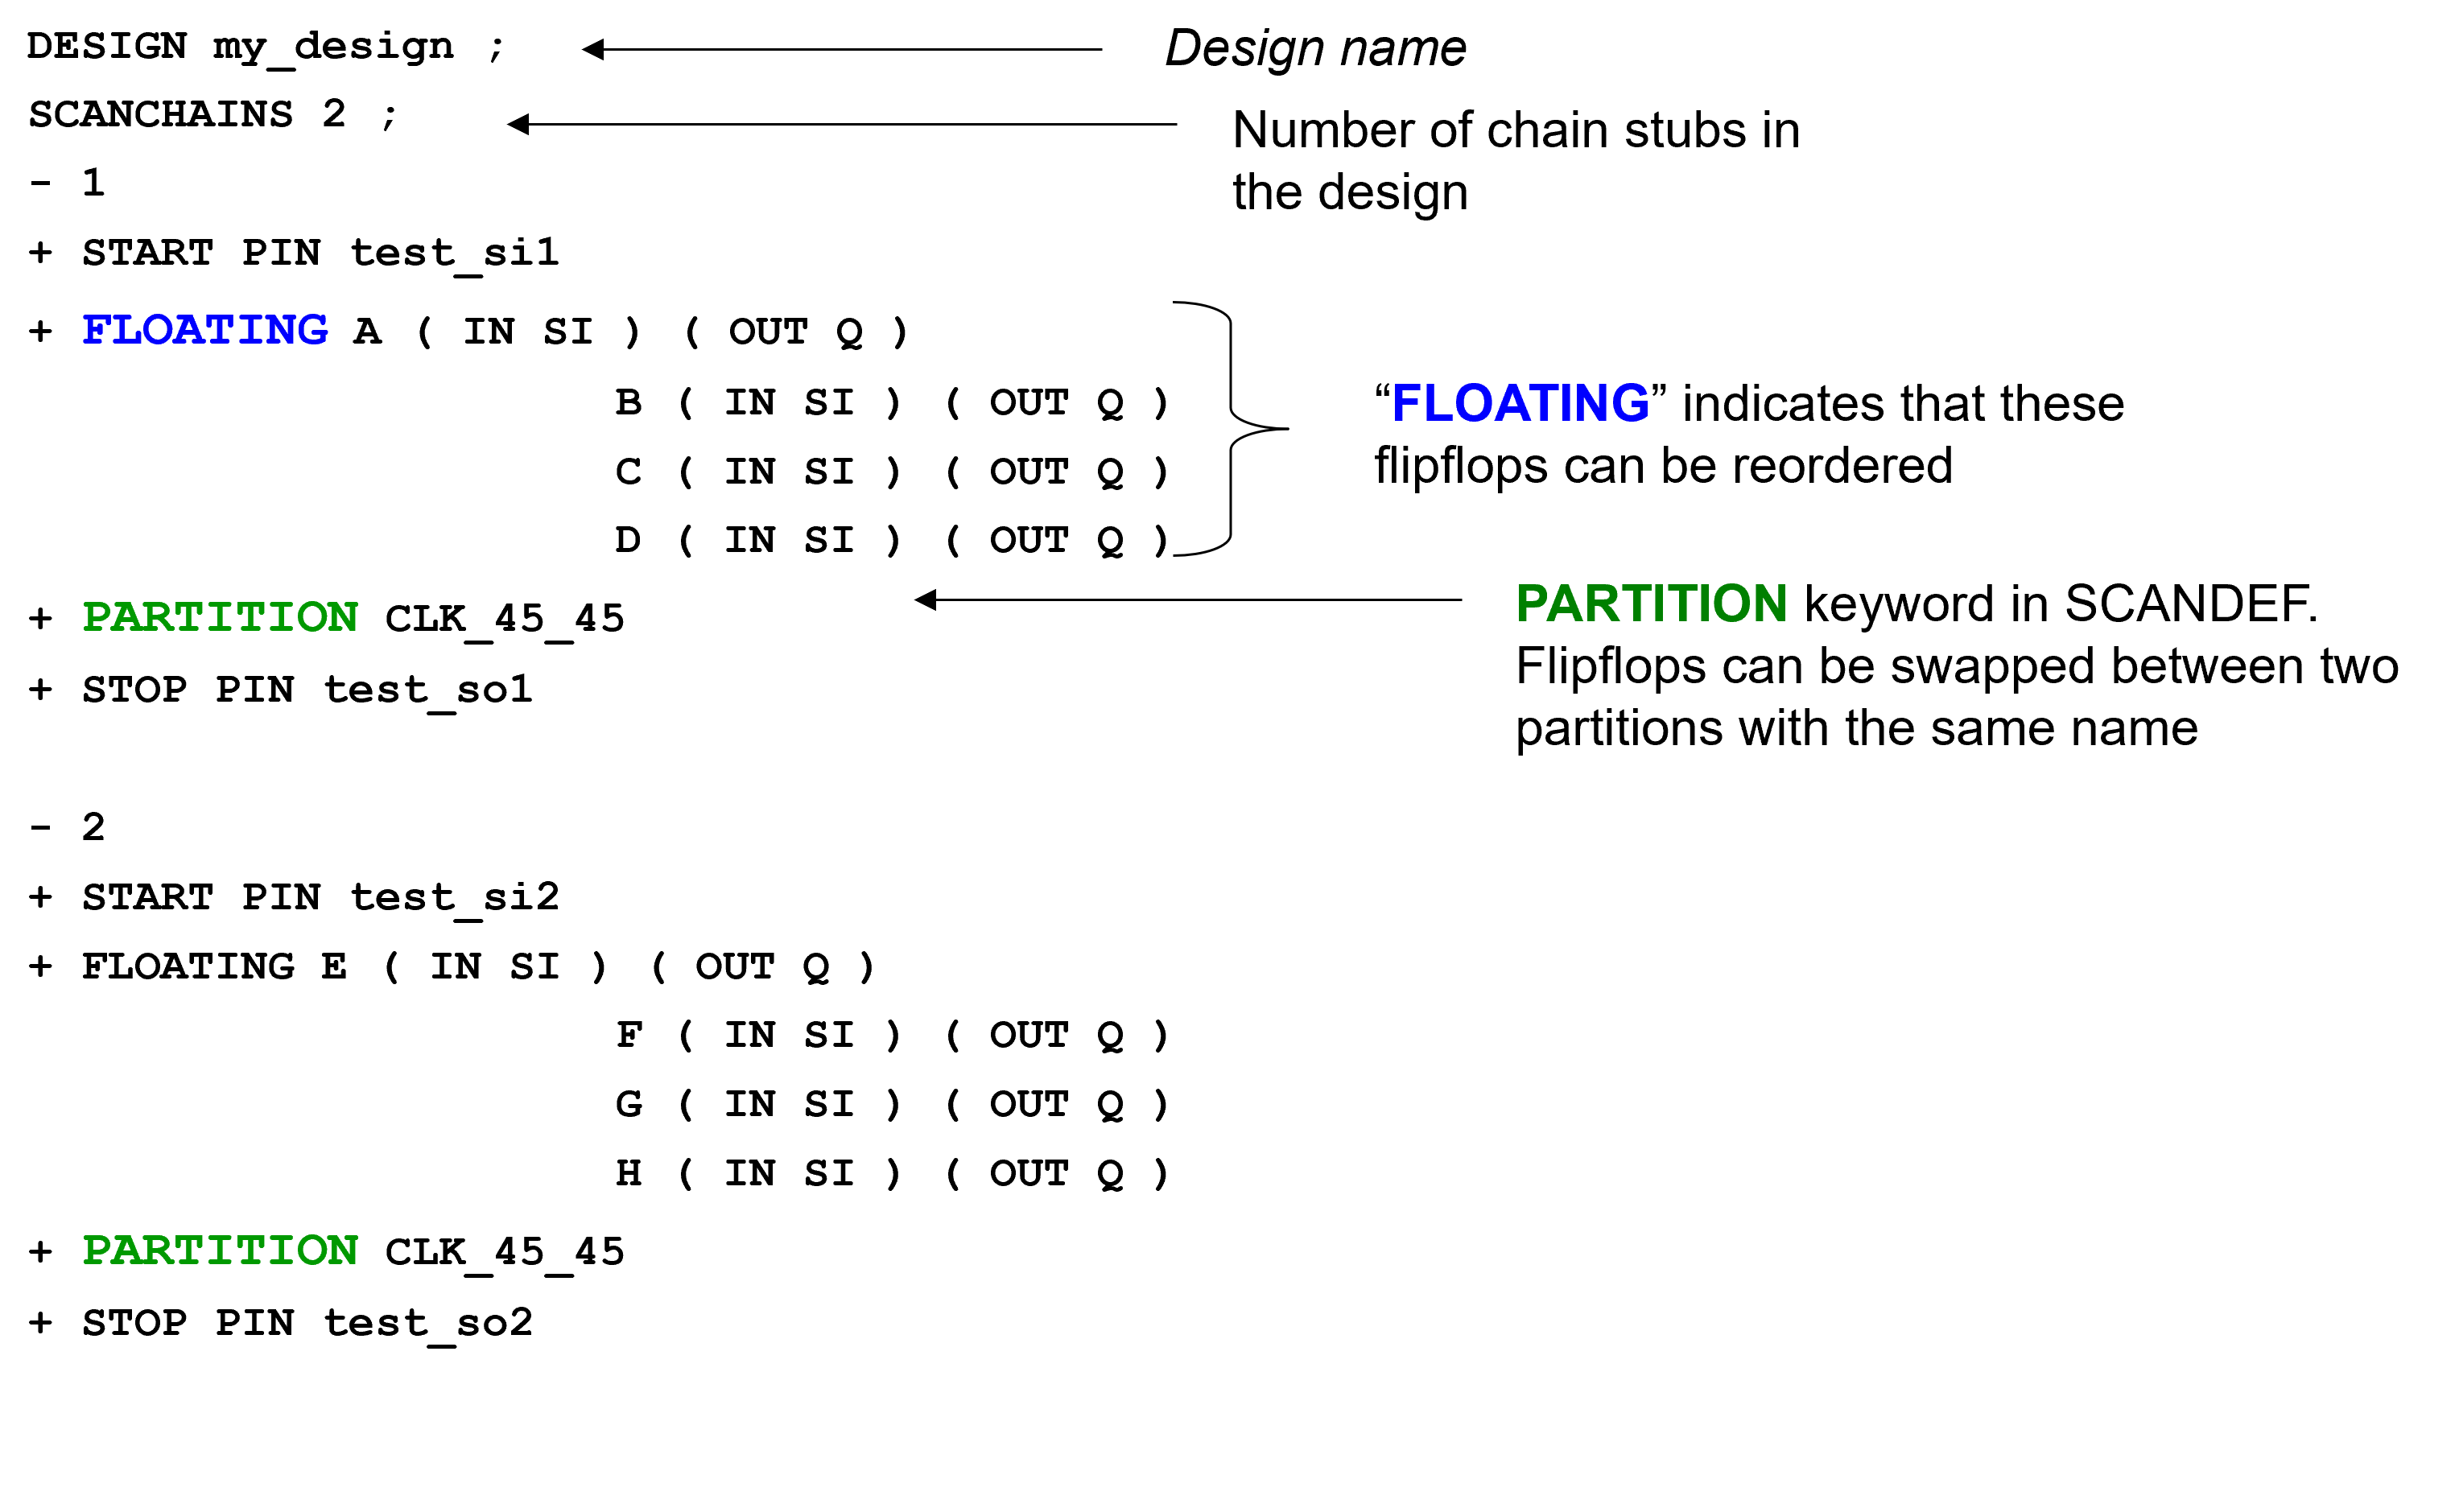
\includegraphics[width=\textwidth]{SC5}
	\end{center}
\end{frame}

\begin{frame}
	\frametitle{Alpha-Numeric Ordering}
	\begin{center}
		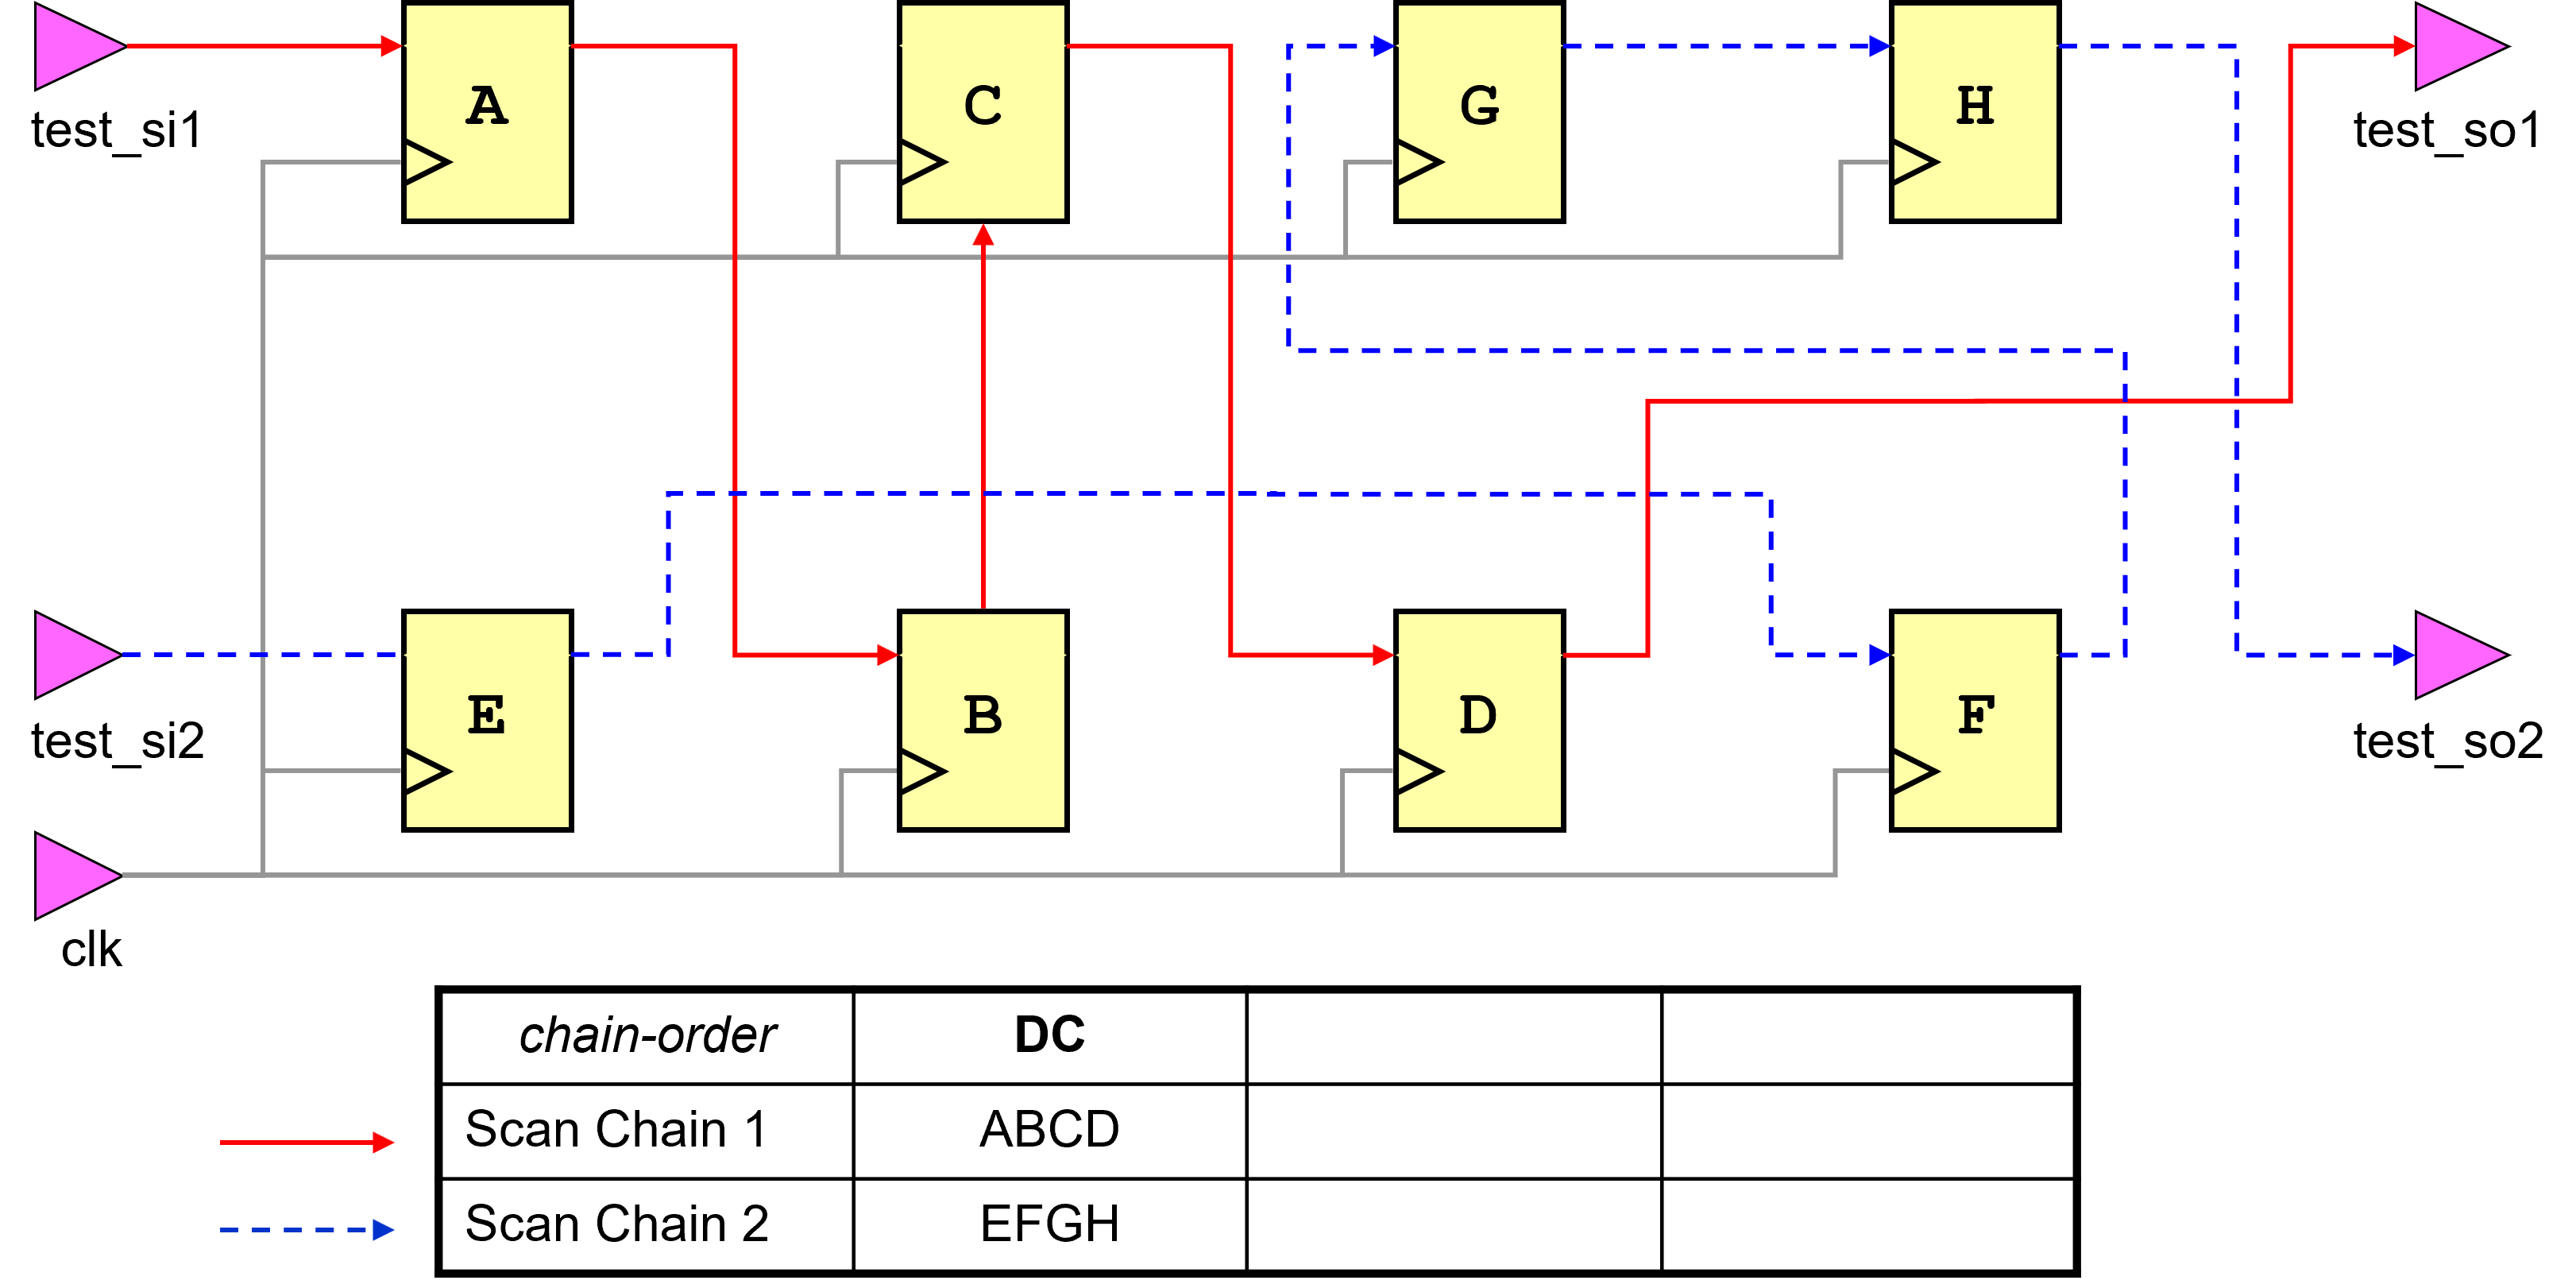
\includegraphics[width=\textwidth]{SC6}
	\end{center}
\end{frame}

\begin{frame}
	\frametitle{Reordering Within Scan-Chain}
	\begin{center}
		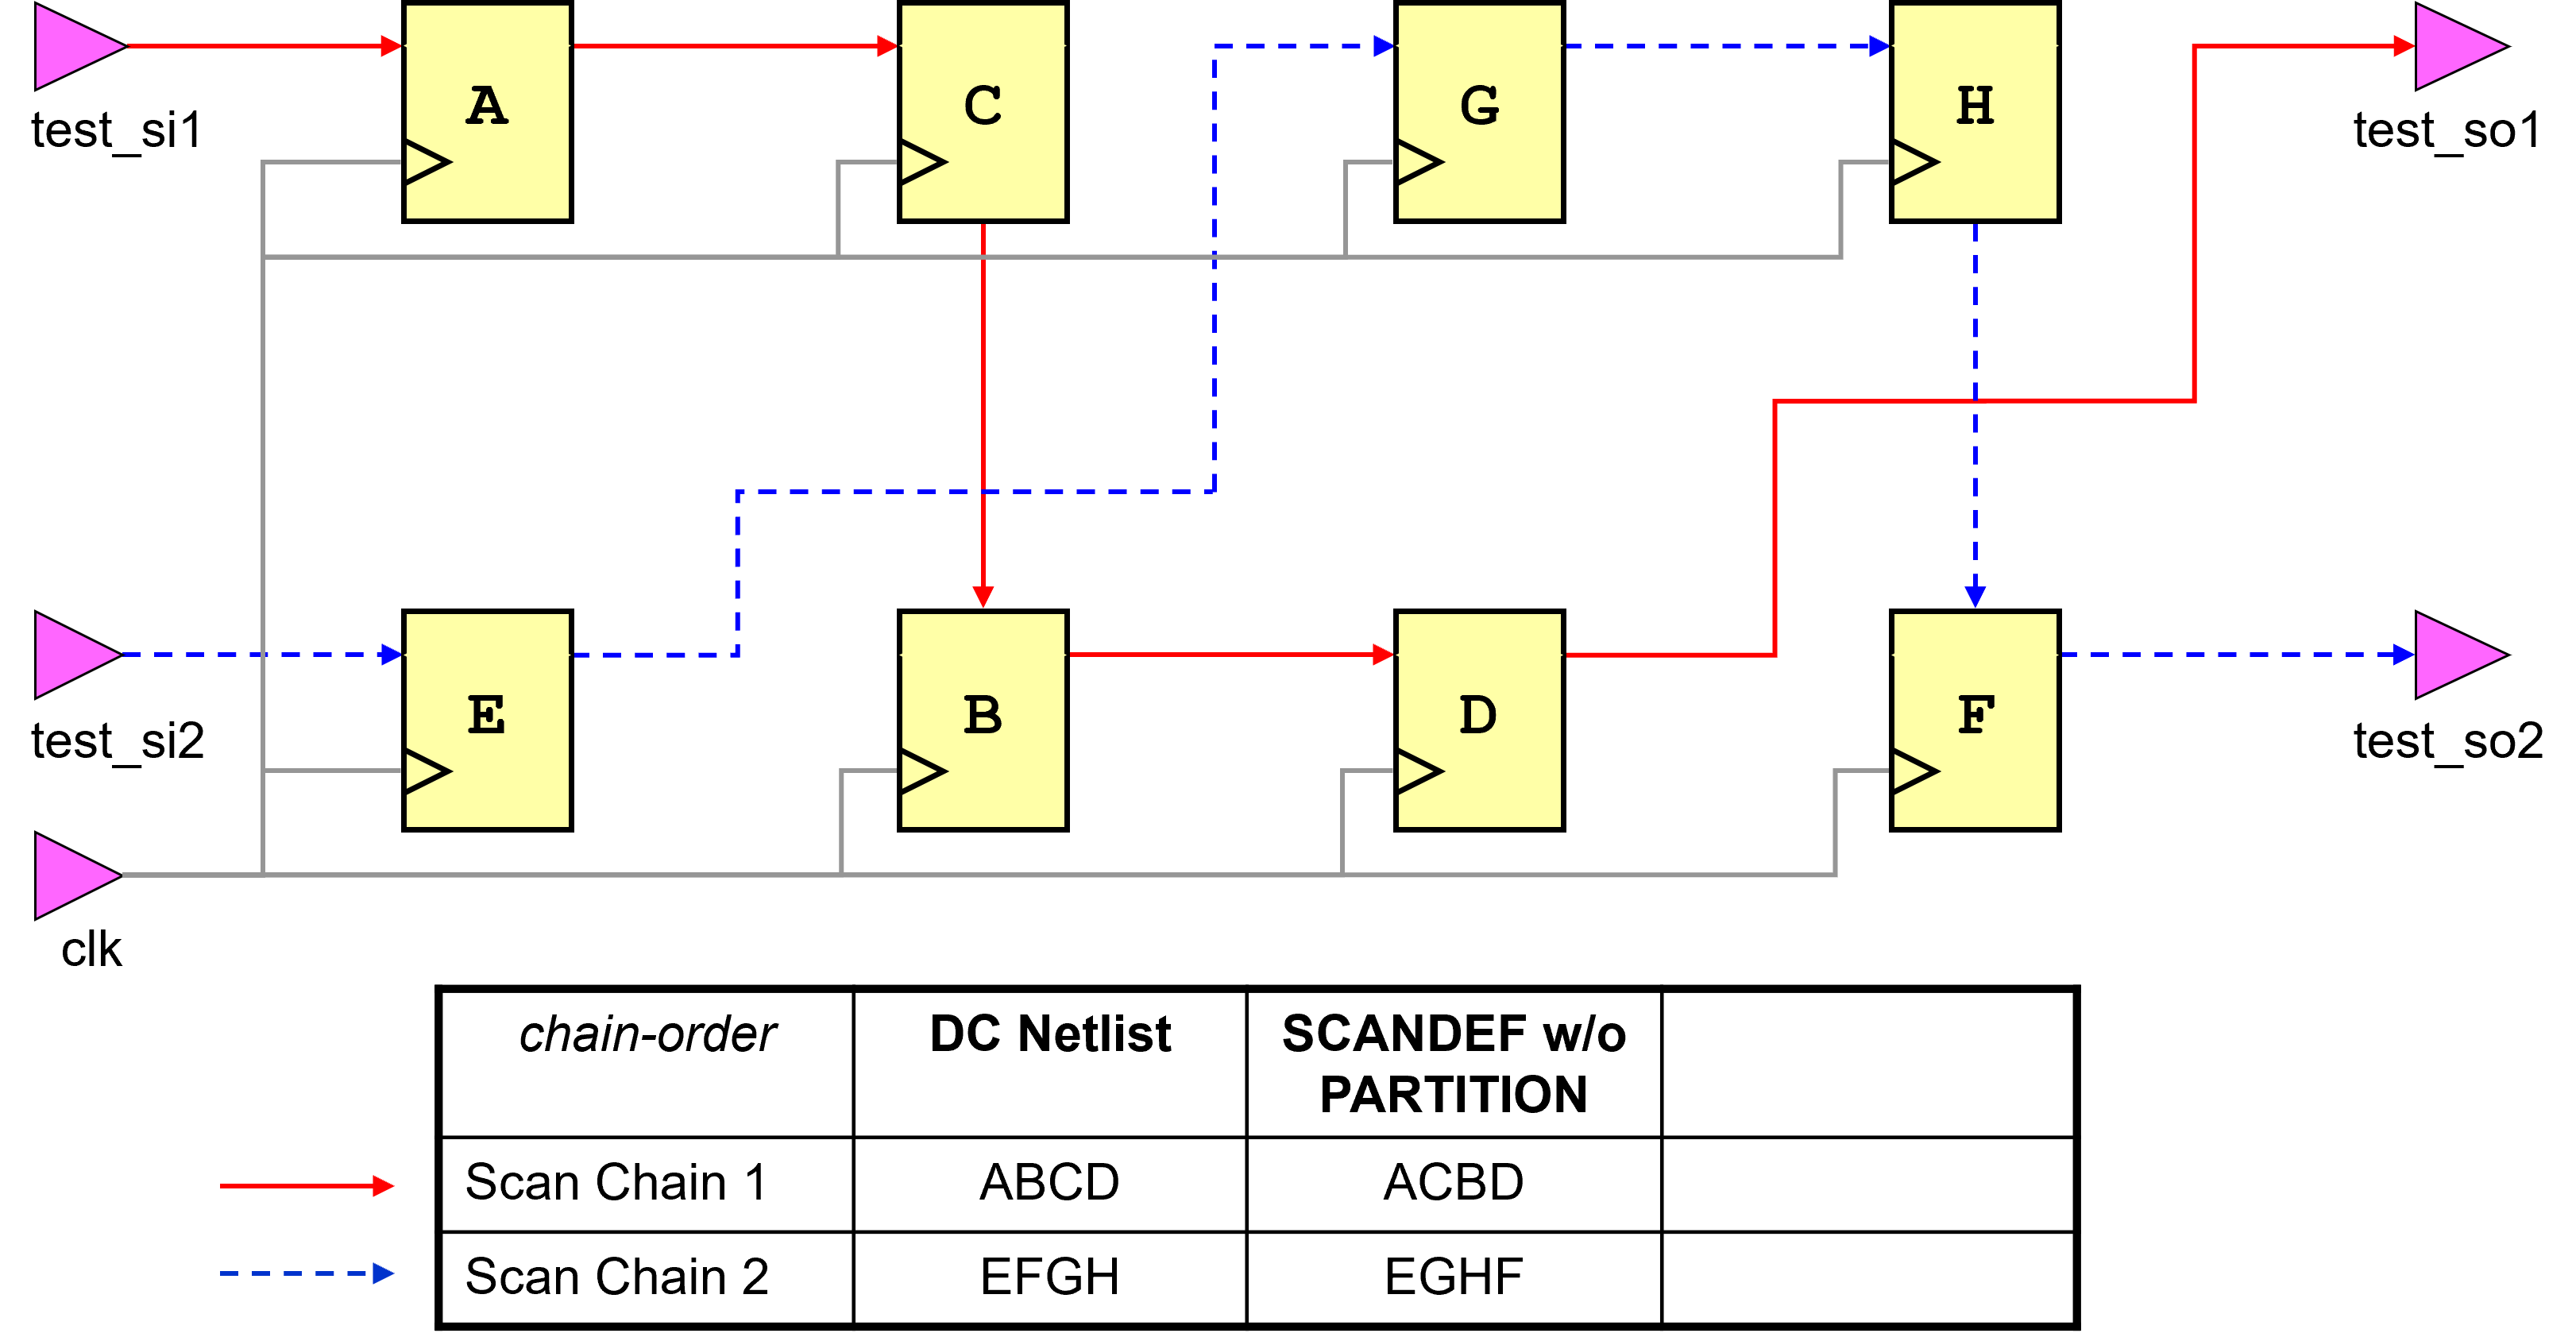
\includegraphics[width=\textwidth]{SC7}
	\end{center}
\end{frame}
\begin{frame}
	\frametitle{Reordering Across Scan-Chains}
	\begin{center}
		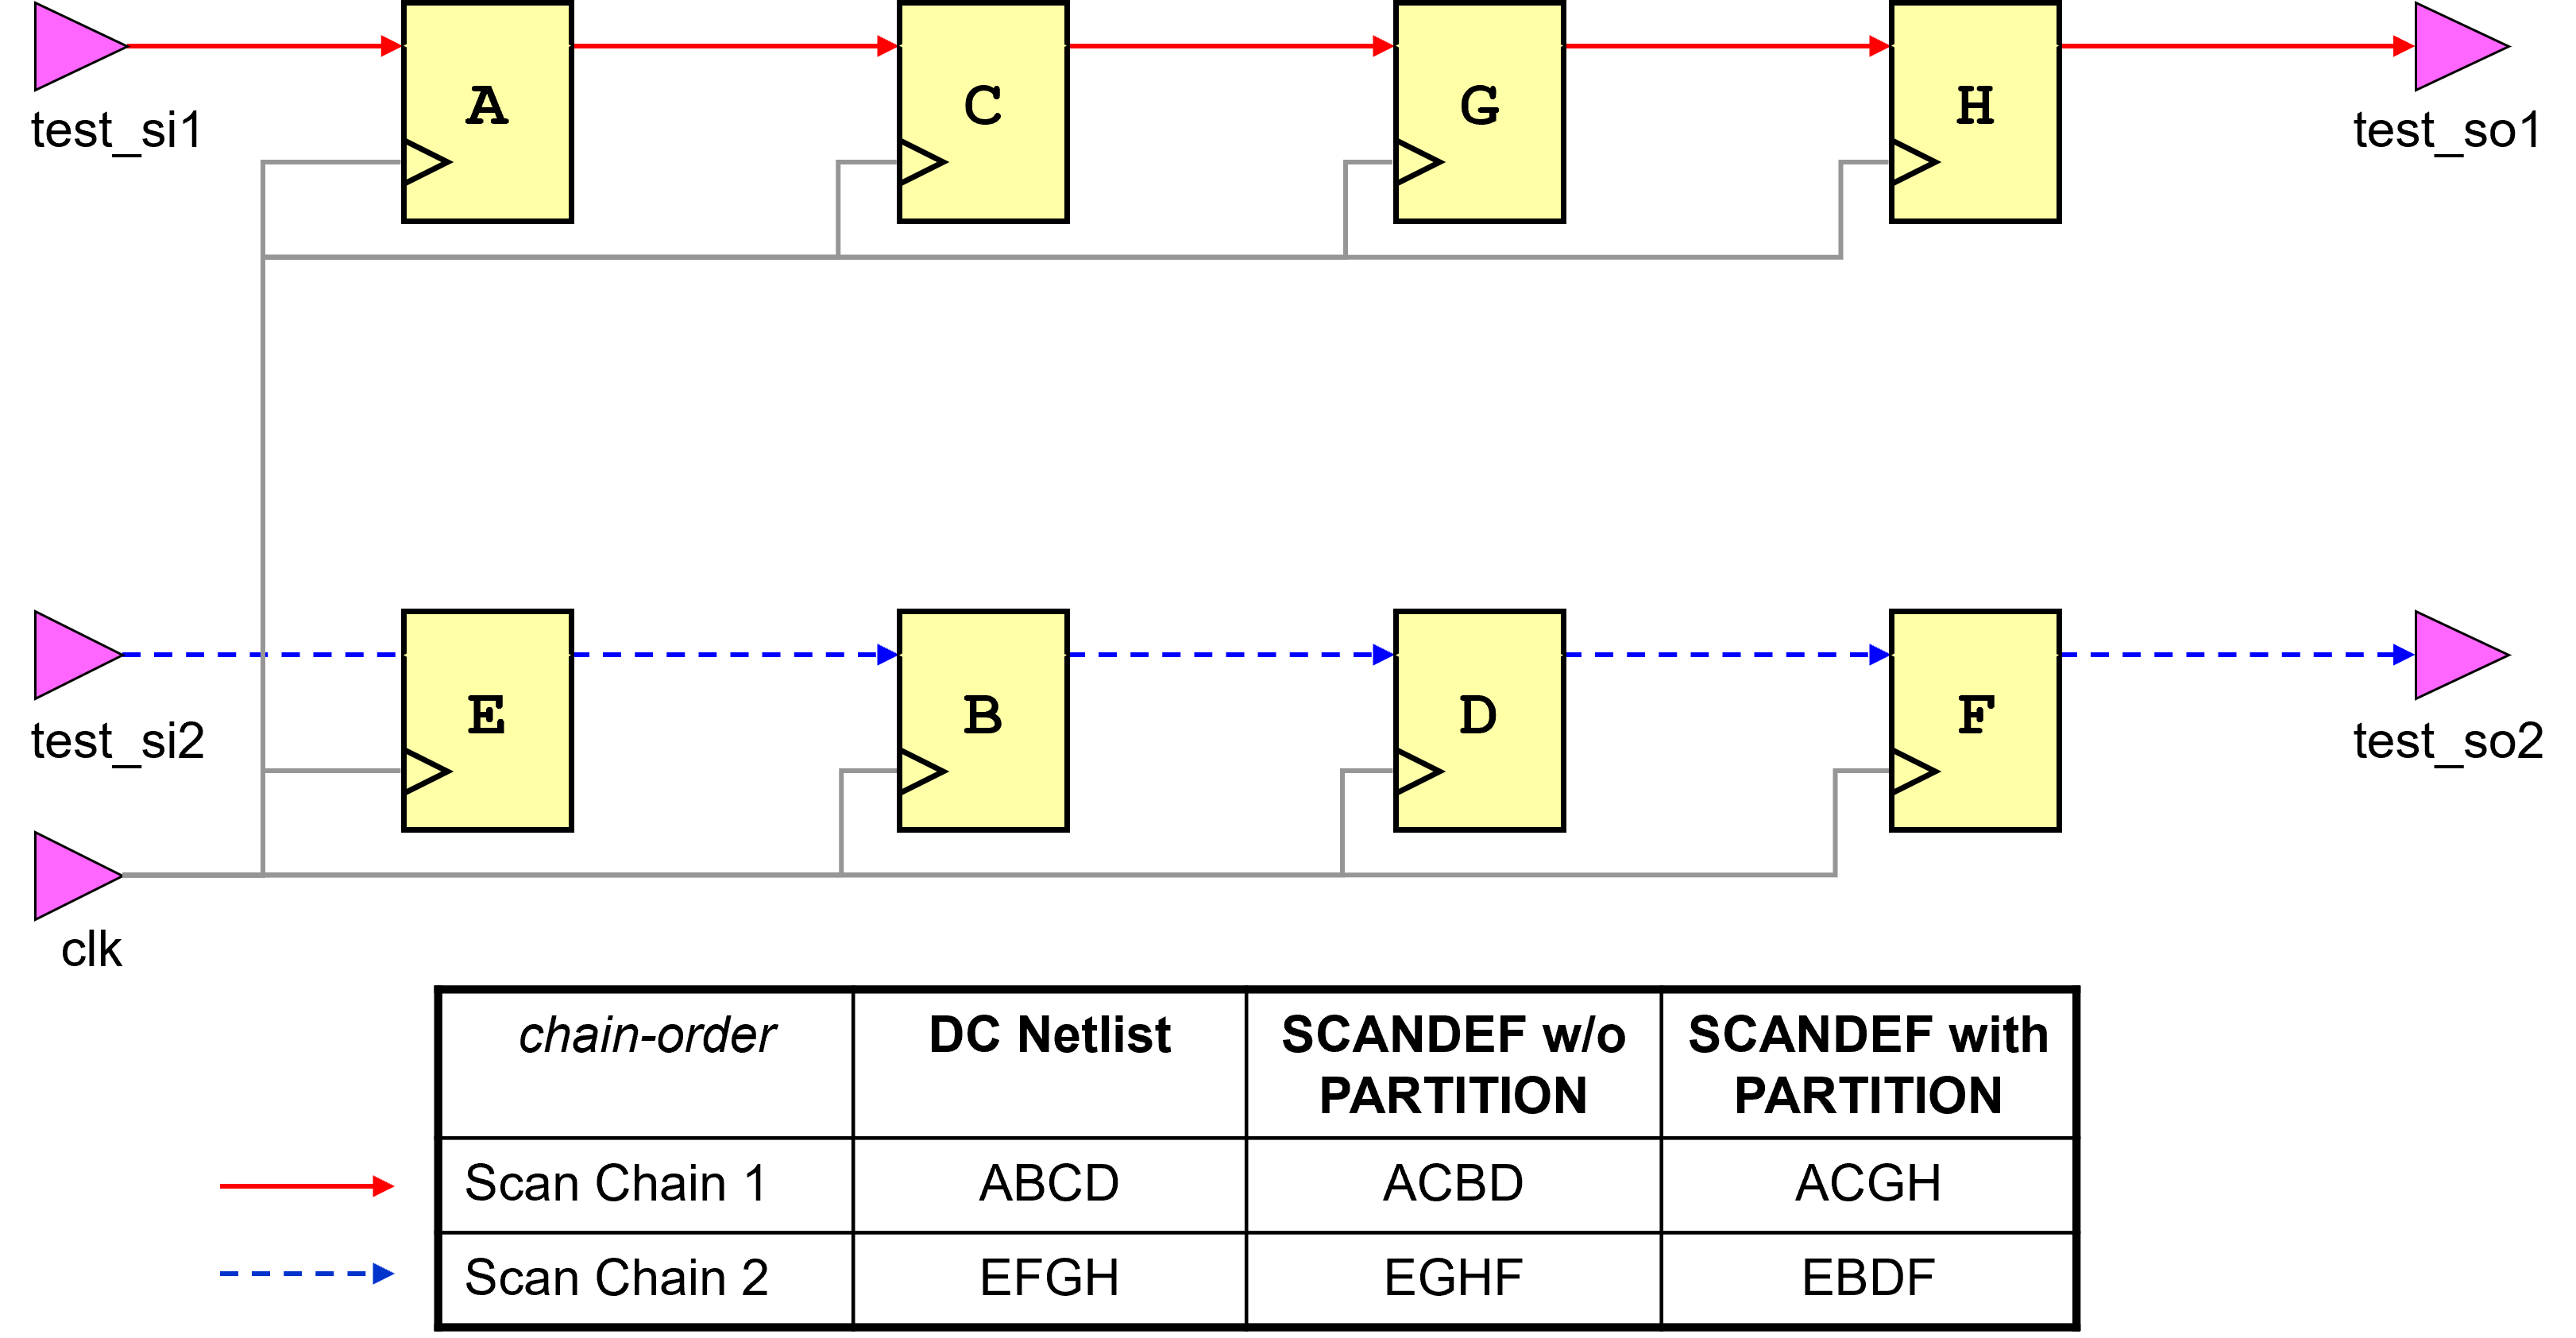
\includegraphics[width=\textwidth]{SC8}
	\end{center}
\end{frame}


\section[Optimization]{Placement Optimization}
\subsection[Optimization]{Placement Optimization}

\begin{frame}
	\frametitle{Optimization techniques}
	\begin{center}
		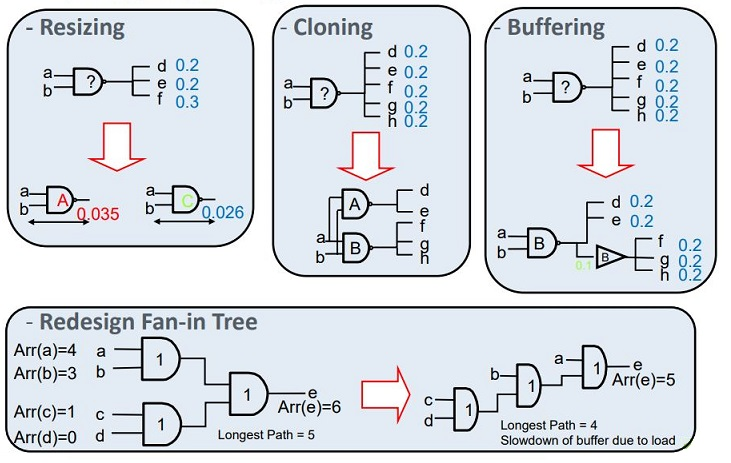
\includegraphics[width=\textwidth]{Placement-optimization2}
	\end{center}
\end{frame}
\begin{frame}
	\frametitle{Optimization techniques}
	\begin{center}
		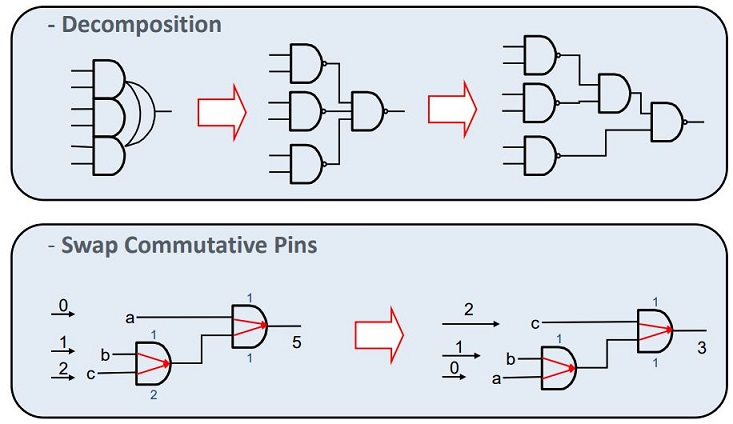
\includegraphics[width=\textwidth]{Placement-optimization}
	\end{center}
\end{frame}
\begin{frame}
	\frametitle{No Hold Time Fixing}
	\begin{itemize}
		\item By default \textcolor{red}{place\_opt} tries to fix only setup time
		violations - No hold time fixing
		\item Hold time will be addressed during clock tree
		synthesis
		\item All timing calculations are based on ideal clocks (clock skew = 0). Therefore,
		it is a common practice to give more constrained timing to placement
		engine with:
		\begin{enumerate}
			\item Extra uncertainty
			\item Frequency Overdrive
		\end{enumerate}
	\end{itemize}
\end{frame}
%---------------------------------------------------	
\begin{frame}
	\frametitle{....}
	\begin{center}
		\<بِسْمِ اللَّـهِ الرَّحْمَـٰنِ الرَّحِيمِ> \\
		\<وَمَا أُوتِيتُمْ مِنَ الْعِلْمِ إِلَّا قَلِيلًا>
		
	\end{center}
\end{frame}
%---------------------------------------------	
\end{document}	